\documentclass[]{book}
\usepackage{lmodern}
\usepackage{amssymb,amsmath}
\usepackage{ifxetex,ifluatex}
\usepackage{fixltx2e} % provides \textsubscript
\ifnum 0\ifxetex 1\fi\ifluatex 1\fi=0 % if pdftex
  \usepackage[T1]{fontenc}
  \usepackage[utf8]{inputenc}
\else % if luatex or xelatex
  \ifxetex
    \usepackage{mathspec}
  \else
    \usepackage{fontspec}
  \fi
  \defaultfontfeatures{Ligatures=TeX,Scale=MatchLowercase}
\fi
% use upquote if available, for straight quotes in verbatim environments
\IfFileExists{upquote.sty}{\usepackage{upquote}}{}
% use microtype if available
\IfFileExists{microtype.sty}{%
\usepackage{microtype}
\UseMicrotypeSet[protrusion]{basicmath} % disable protrusion for tt fonts
}{}
\usepackage[margin=1in]{geometry}
\usepackage{hyperref}
\hypersetup{unicode=true,
            pdftitle={Mál- og tegurfræði},
            pdfauthor={Brynjólfur Gauti Jónsson},
            pdfborder={0 0 0},
            breaklinks=true}
\urlstyle{same}  % don't use monospace font for urls
\usepackage{natbib}
\bibliographystyle{plainnat}
\usepackage{color}
\usepackage{fancyvrb}
\newcommand{\VerbBar}{|}
\newcommand{\VERB}{\Verb[commandchars=\\\{\}]}
\DefineVerbatimEnvironment{Highlighting}{Verbatim}{commandchars=\\\{\}}
% Add ',fontsize=\small' for more characters per line
\usepackage{framed}
\definecolor{shadecolor}{RGB}{248,248,248}
\newenvironment{Shaded}{\begin{snugshade}}{\end{snugshade}}
\newcommand{\AlertTok}[1]{\textcolor[rgb]{0.94,0.16,0.16}{#1}}
\newcommand{\AnnotationTok}[1]{\textcolor[rgb]{0.56,0.35,0.01}{\textbf{\textit{#1}}}}
\newcommand{\AttributeTok}[1]{\textcolor[rgb]{0.77,0.63,0.00}{#1}}
\newcommand{\BaseNTok}[1]{\textcolor[rgb]{0.00,0.00,0.81}{#1}}
\newcommand{\BuiltInTok}[1]{#1}
\newcommand{\CharTok}[1]{\textcolor[rgb]{0.31,0.60,0.02}{#1}}
\newcommand{\CommentTok}[1]{\textcolor[rgb]{0.56,0.35,0.01}{\textit{#1}}}
\newcommand{\CommentVarTok}[1]{\textcolor[rgb]{0.56,0.35,0.01}{\textbf{\textit{#1}}}}
\newcommand{\ConstantTok}[1]{\textcolor[rgb]{0.00,0.00,0.00}{#1}}
\newcommand{\ControlFlowTok}[1]{\textcolor[rgb]{0.13,0.29,0.53}{\textbf{#1}}}
\newcommand{\DataTypeTok}[1]{\textcolor[rgb]{0.13,0.29,0.53}{#1}}
\newcommand{\DecValTok}[1]{\textcolor[rgb]{0.00,0.00,0.81}{#1}}
\newcommand{\DocumentationTok}[1]{\textcolor[rgb]{0.56,0.35,0.01}{\textbf{\textit{#1}}}}
\newcommand{\ErrorTok}[1]{\textcolor[rgb]{0.64,0.00,0.00}{\textbf{#1}}}
\newcommand{\ExtensionTok}[1]{#1}
\newcommand{\FloatTok}[1]{\textcolor[rgb]{0.00,0.00,0.81}{#1}}
\newcommand{\FunctionTok}[1]{\textcolor[rgb]{0.00,0.00,0.00}{#1}}
\newcommand{\ImportTok}[1]{#1}
\newcommand{\InformationTok}[1]{\textcolor[rgb]{0.56,0.35,0.01}{\textbf{\textit{#1}}}}
\newcommand{\KeywordTok}[1]{\textcolor[rgb]{0.13,0.29,0.53}{\textbf{#1}}}
\newcommand{\NormalTok}[1]{#1}
\newcommand{\OperatorTok}[1]{\textcolor[rgb]{0.81,0.36,0.00}{\textbf{#1}}}
\newcommand{\OtherTok}[1]{\textcolor[rgb]{0.56,0.35,0.01}{#1}}
\newcommand{\PreprocessorTok}[1]{\textcolor[rgb]{0.56,0.35,0.01}{\textit{#1}}}
\newcommand{\RegionMarkerTok}[1]{#1}
\newcommand{\SpecialCharTok}[1]{\textcolor[rgb]{0.00,0.00,0.00}{#1}}
\newcommand{\SpecialStringTok}[1]{\textcolor[rgb]{0.31,0.60,0.02}{#1}}
\newcommand{\StringTok}[1]{\textcolor[rgb]{0.31,0.60,0.02}{#1}}
\newcommand{\VariableTok}[1]{\textcolor[rgb]{0.00,0.00,0.00}{#1}}
\newcommand{\VerbatimStringTok}[1]{\textcolor[rgb]{0.31,0.60,0.02}{#1}}
\newcommand{\WarningTok}[1]{\textcolor[rgb]{0.56,0.35,0.01}{\textbf{\textit{#1}}}}
\usepackage{longtable,booktabs}
\usepackage{graphicx,grffile}
\makeatletter
\def\maxwidth{\ifdim\Gin@nat@width>\linewidth\linewidth\else\Gin@nat@width\fi}
\def\maxheight{\ifdim\Gin@nat@height>\textheight\textheight\else\Gin@nat@height\fi}
\makeatother
% Scale images if necessary, so that they will not overflow the page
% margins by default, and it is still possible to overwrite the defaults
% using explicit options in \includegraphics[width, height, ...]{}
\setkeys{Gin}{width=\maxwidth,height=\maxheight,keepaspectratio}
\IfFileExists{parskip.sty}{%
\usepackage{parskip}
}{% else
\setlength{\parindent}{0pt}
\setlength{\parskip}{6pt plus 2pt minus 1pt}
}
\setlength{\emergencystretch}{3em}  % prevent overfull lines
\providecommand{\tightlist}{%
  \setlength{\itemsep}{0pt}\setlength{\parskip}{0pt}}
\setcounter{secnumdepth}{5}
% Redefines (sub)paragraphs to behave more like sections
\ifx\paragraph\undefined\else
\let\oldparagraph\paragraph
\renewcommand{\paragraph}[1]{\oldparagraph{#1}\mbox{}}
\fi
\ifx\subparagraph\undefined\else
\let\oldsubparagraph\subparagraph
\renewcommand{\subparagraph}[1]{\oldsubparagraph{#1}\mbox{}}
\fi

%%% Use protect on footnotes to avoid problems with footnotes in titles
\let\rmarkdownfootnote\footnote%
\def\footnote{\protect\rmarkdownfootnote}

%%% Change title format to be more compact
\usepackage{titling}

% Create subtitle command for use in maketitle
\providecommand{\subtitle}[1]{
  \posttitle{
    \begin{center}\large#1\end{center}
    }
}

\setlength{\droptitle}{-2em}

  \title{Mál- og tegurfræði}
    \pretitle{\vspace{\droptitle}\centering\huge}
  \posttitle{\par}
    \author{Brynjólfur Gauti Jónsson}
    \preauthor{\centering\large\emph}
  \postauthor{\par}
      \predate{\centering\large\emph}
  \postdate{\par}
    \date{2019-03-21}

\usepackage{booktabs}

\begin{document}
\maketitle

{
\setcounter{tocdepth}{1}
\tableofcontents
}
\hypertarget{kennsluatlun}{%
\chapter*{Kennsluáætlun}\label{kennsluatlun}}
\addcontentsline{toc}{chapter}{Kennsluáætlun}

\begin{itemize}
\item
  \textbf{Vika 1:} Mengjafræði, aukna rauntalnalínan, raðir.
\item
  \textbf{Vika 2:} Jordan-mælanleg mengi, tröppuföll, Riemann-heildi.
\item
  \textbf{Vika 3:} Legesbue: Utanmálið, mælanleg mengi og málið.
\item
  \textbf{Vika 4:} Málrúm
\item
  \textbf{Vika 5:}
\item
  \textbf{Vika 6:}
\item
  \textbf{Vika 7:} Heildanleg föll
\item
  \textbf{Vika 8:}
\item
  \textbf{Vika 9:}
\end{itemize}

\hypertarget{orlitil-mengjafri}{%
\chapter{Örlítil mengjafræði}\label{orlitil-mengjafri}}

Gefum okkur að til grundvallar liggi \emph{hæfilega stórt} almengi.

\hypertarget{skilgreining}{%
\section{Skilgreining}\label{skilgreining}}

\textbf{Fjölskylda} af hlutmengjum í mengi \(M\) er vörpun

\[
a: I\rightarrow \mathcal P(M).
\]

Við notum yfirleitt tákn af greðinni \(A_i\) til þess að tákna gildi vörpunarinnar \(a\) í \(i\) og vörpunina \(a\) táknum við þá \((A_i)_{i\in I}\).

Við köllum \(I\) \textbf{stikamengi} fjölskyldunnar.

Mengið

\[
\bigcap_{i\in I}A_i := \{x\in M| x \in A_i \text{ fyrir öll } i\in I\}
\]

kallast \textbf{sniðmengi} fjölskyldunnar.

Mengið

\[
\bigcup_{i\in I}A_i := \{x\in M| x \in A_i \text{ fyrir eitthvert } i\in I\}
\]

kallast \textbf{sammengi} fjölskyldunnar.

Fyrir hlutmengi \(A\) í \(M\) setjum við

\[
A^c := M\backslash A := \{x \in M | x \notin A\}
\]

og köllum \textbf{fyllimengi} \(A\) (í \(M\)).

\begin{center}\rule{0.5\linewidth}{\linethickness}\end{center}

Ef \(B\) er líka hlutmengi í \(M\), þá setjum við

\[
B\backslash A := \{x \in B| x \notin A\} = B \cup A^c
\]

og hlutmengið

\[
A\Delta B := (A\backslash B) \cup (B\backslash A)
\]

köllum við \textbf{samhverfan mismun} hlutmengjanna \(A\) og \(B\).

\begin{center}\rule{0.5\linewidth}{\linethickness}\end{center}

Um sérhverja fjölskyldu \((A_i)_{i\in I}\) í mengi M gilda \textbf{reglur de Morgans}

\[
\big(\bigcup_{i\in I} A_i\big)^c = \bigcap_{i\in I}A_i^c \\
\big(\bigcap_{i\in I} A_i\big)^c = \bigcup_{i\in I}A_i^c
\]

\begin{center}\rule{0.5\linewidth}{\linethickness}\end{center}

\textbf{Kennifall} hlutmengis A í M er táknað \(\mathbf 1_A: M \rightarrow \mathbb R\) og skilgreint með því að setja \(\mathbf 1_A(x) := 1\) ef \(x\in A\) og \(\mathbf 1_A(x) = 0\) ef \(x \notin A\).

Fyrir hlutmengi A og B í M gilda reglurnar

\begin{itemize}
\item
  \(\mathbf 1_{A\cap B} = \mathbf 1_A \mathbf 1_B\)
\item
  \(\mathbf 1_{A\cup B} = \mathbf 1_A + \mathbf 1_B - \mathbf 1_A\mathbf 1_B\)
\item
  \(\mathbf 1_{A^c} = 1 - \mathbf 1_A\)
\end{itemize}

\hypertarget{aukna-rauntalnalinan}{%
\chapter{Aukna rauntalnalínan}\label{aukna-rauntalnalinan}}

Við köllum mengið \(\overline{\mathbb R} := \mathbb R \cup \{-\infty, \infty\} = [-\infty, \infty]\) \textbf{auknu rauntalnalínuna}. Við framlengjum röðuna á \(\mathbb R\) yfir á \(\overline{\mathbb R}\) með skilyrðinu

\[
-\infty < x < \infty \text{ fyrir öll x úr } \mathbb R
\]

og framlengjum venjulegu reikniaðgerðirnar á \(\mathbb R\) yfir á \(\overline{\mathbb R}\) með því að setja:

\begin{itemize}
\item
  \(a + \infty = \infty \text{ fyrir öll } a\in (-\infty, \infty]\)
\item
  \(a + (-\infty) = -\infty \text{ fyrir öll } a\in [-\infty, \infty)\)
\item
  \(a \cdot \infty = \infty \text{ og } a \cdot (-\infty) = -\infty \text{ fyrir öll } a\in (0, \infty]\)
\item
  \(a \cdot \infty = -\infty \text{ og } a \cdot (-\infty) = \infty \text{ fyrir öll } a\in [-\infty, 0)\)
\end{itemize}

\begin{center}\rule{0.5\linewidth}{\linethickness}\end{center}

Látum A vera hlutmengi í \(\overline{\mathbb R}\)

\begin{itemize}
\item
  Minnsta yfirstak mengisins A í \(\overline{\mathbb R}\) kallast \textbf{efra mark} mengisins A og við táknum það \(\sup A\).
\item
  Stærsta undirstak mengisins A í \(\overline{\mathbb R}\) kallast \textbf{neðra mark} mengisins A og við táknum það \(\inf A\).
\end{itemize}

Ef \((x_n)_{n\geq 0}\) er runa í \(\overline{\mathbb R}\) og \(n_0 \in \mathbb N\), þá setjum við

\begin{itemize}
\item
  \(\sup_{n\geq n_0}x_n := \sup\{x_n | n \geq n_0\}\)
\item
  \(\inf_{n\geq n_0}x_n := \inf\{x_n | n \geq n_0\}\)
\end{itemize}

\begin{center}\rule{0.5\linewidth}{\linethickness}\end{center}

Mengi A í \(\overline{\mathbb R}\) er sagt \textbf{takmarkað að ofan {[}neðan{]}} ef \(\sup A < \infty [\inf A > -\infty]\). Samsvarandi fyrir runur.

\hypertarget{efra--og-nera-markgildi-runu}{%
\section{Efra- og neðra markgildi runu}\label{efra--og-nera-markgildi-runu}}

Látum \((x_n)\) vera runu í \(\overline{\mathbb R}\). Þá er runan \(\big(\sup_{n\geq k}x_n\big)_k\) minnkandi og hefur því markgildi í \(\overline{\mathbb R}\). Við setjum

\[
\limsup x_n := \lim_{k\rightarrow \infty}\sup_{n\geq k}x_n
\]

og köllum \(\limsup x_n\) \textbf{efra markgildi} rununnar \((x_n)\).

Með svipuðum rökum er unnt að skilgreina stakið

\[
\liminf x_n := \lim_{k\rightarrow \infty}\inf_{n\geq k}x_n.
\]

Það kallast \textbf{neðra markgildi} rununnar \((x_n)\).

\hypertarget{setning}{%
\section{Setning}\label{setning}}

Látum \((x_n)\) vera runu í \(\overline{\mathbb R}\) og E vera mengi allra staka úr \(\overline{\mathbb R}\) sem eru markgildi einhverrar hlutrunu í \((x_n)\). Þá gildir

\[
\limsup x_n = \max E \quad \text{og} \quad \liminf x_n = \min E
\]

\hypertarget{setning-1}{%
\section{Setning}\label{setning-1}}

Látum \((x_n)\) vera runu í \(\overline{\mathbb R}\). Þá gilda eftirfarandi jöfnur og ójöfnur:

\emph{(i)} \(\limsup (-x_n) = -\liminf x_n\) og \(\liminf (-x_n) = -\limsup x_n\).

\emph{(ii)} \(\liminf x_n \leq \limsup x_n\).

Ennfremur gildir að runan \((x_n)\) er samleitin þá og því aðeins að \(\liminf x_n = \limsup x_n\).

\hypertarget{setning-2}{%
\section{Setning}\label{setning-2}}

Látum \((x_n)\) og \((y_n)\) vera runur í \(\overline{\mathbb R}\) sem hafa þann eiginleika að \(x_n \leq y_n\) fyrir öll \(n\), þá fæst \(\liminf x_n \leq \liminf y_n\) og \(\limsup x_n \leq \limsup y_n\).

\hypertarget{setning-3}{%
\section{Setning}\label{setning-3}}

Látum \((x_n)\) og \((y_n)\) vera runur í \(\overline{\mathbb R}\), þá gilda ójöfnurnar

\[
\begin{aligned}
\liminf x_n + \liminf y_n &\leq \liminf(x_n + y_n) \\
&\leq \liminf x_n + \limsup y_n \\
&\leq \limsup(x_n + y_n) \\
&\leq \limsup x_n + \limsup y_n
\end{aligned}
\]

\hypertarget{nokkur-atrii-varnandi-rair}{%
\chapter{Nokkur atriði varnandi raðir}\label{nokkur-atrii-varnandi-rair}}

\hypertarget{setning-4}{%
\section{Setning}\label{setning-4}}

Látum \((a_n)_{n\geq 0}\) vera runu í \([0, \infty]\) og látum \(\mathcal S\) tákna mengi allra summa af gerðinni \(\sum_{n\in I}a_n\) þar sem I er endanlegt hlutmengi í \(\mathbb N\). Þá gildir

\[
\sum_{n=0}^\infty a_n = \sup(\mathcal S)
\]

\hypertarget{setning-5}{%
\section{Setning}\label{setning-5}}

Látum \(\sum_{n=0}^\infty a_n\) vera alsamleitna tvinntalnaröð og \(\sigma: \mathbb N \rightarrow \mathbb N\) vera gagntæka vörpum (m.ö.o. \textbf{umröðun}). Þá er röðin \(\sum_{n=0}^\infty a_{\sigma(n)}\) einnig alsamleiting og

\[
\sum_{n=0}^\infty a_{\sigma(n)} = \sum_{n=0}^\infty a_n.
\]

Eftirfarandi setning er einkar áhugaverð í tengslum við setningu 2.1.2, en kemur ekki við sögu í þessu námskeiði.

\hypertarget{umrounarsetning-riemanns}{%
\section{Umröðunarsetning Riemanns}\label{umrounarsetning-riemanns}}

Látum \(\sum_{n=0}^\infty a_n\) vera \emph{skilyrt samleitna} rauntalnaröð og \(c\) og \(d\) vera stök úr \(\overline{\mathbb R}\) þannig að \(c\leq d\). Þá er til umröðum \(\sigma: \mathbb N \rightarrow \mathbb N\), sem hefur þann eiginleika

\[
\liminf \sum_{k=0}^n a_{\sigma(k)} = 0 \quad \text{og} \quad \limsup \sum_{k=0}^n a_{\sigma(k)} = d.
\]

Látum I vera óendanlegt teljanlegt mengi og \((a_i)_{i\in I}\) vera fjölskyldu af tvinntölum. Við segjum að \textbf{summan} \(\sum_{i\in I}a_i\) sé \textbf{alsamleitin} ef til er gagntæk vörpun \(\sigma: \mathbb N \rightarrow I\), sem hefur þann eiginleika að \(\sum_{n=0}^\infty a_{\sigma(n)}\) sé alsamleitin. Sé svo, þá gildir samkvæmt \emph{setningu 2.1.2} að talan \(\sum_{n=0}^\infty a_{\sigma(n)}\) er óháð því hvaða vörpun \(\sigma\) er valin. Við setjum þá

\[
\sum_{i\in I}a_i := \sum_{n=0}^\infty a_{\sigma(n)}
\]

og köllum \textbf{summu} fjölskyldunnar \((a_i)_{i\in I}\)

\hypertarget{fing}{%
\section{Æfing}\label{fing}}

Látum I vera óendanlegt teljanlegt mengi og \((a_i)_{i\in I}\) vera fjölskyldu af tvinntölum.

\emph{(a)} Gerið grein fyrir að summan \(\sum_{i\in I}a_i\) sé alsamleitin þá og því aðeins að til sé rauntala K, sem hefur þann eiginleika að

\[
\sum_{i\in F} |a_i| \leq K
\]

fyrir sérhvert endanlegt hlutmengi F í I.

\emph{(b)} Gerum ráð fyrir að summan \(\sum_{i\in I}a_i\) sé alsamleitin og setjum \(A:= \sum_{i\in I}a_i\). Sýnið að fyrir sérhvert \(\varepsilon > 0\) sé til endanlegt hlutmengi F í I, sem hefur þann eiginleika að

\[
|\sum_{i\in J}a_i - A| < \varepsilon
\]

fyrir sérhvert endanlegt hlutmengi J í I sem inniheldur F.

\hypertarget{setning-6}{%
\section{Setning}\label{setning-6}}

Tvinntalnasumma \(\sum_{(m,n)\in \mathbb N^2}a_{m,n}\) er alsamleitin þá og því aðeins að

\[
\sum_{m=0}^\infty(\sum_{n=0}^\infty|a_{m,n}|) < \infty,
\]

og sé svo þá gildir

\[
\sum_{(m,n)\in\mathbb N^2} a_{m,n} = \sum_{m=0}^\infty(\sum_{n=0}^\infty a_{m,n})  = \sum_{n=0}^\infty(\sum_{m=0}^\infty a_{m,n})
\]

\hypertarget{setning-7}{%
\section{Setning}\label{setning-7}}

Fyrir sérhverja fjölskyldu \((a_{m,n})_{(m,n)\in \mathbb N^2}\) í \([0, \infty]\) gildir

\[
\sum_{(m,n)\in\mathbb N^2}a_{m,n} = \sum_{m=0}^\infty(\sum_{n=0}^\infty a_{m,n})  = \sum_{n=0}^\infty(\sum_{m=0}^\infty a_{m,n})
\]

\hypertarget{vikubla-1}{%
\chapter*{Vikublað 1}\label{vikubla-1}}
\addcontentsline{toc}{chapter}{Vikublað 1}

\hypertarget{dmi-1}{%
\subsection*{Dæmi 1}\label{dmi-1}}
\addcontentsline{toc}{subsection}{Dæmi 1}

Látum \((x_n)\) vera runu í \(\mathbb R\) og M vera rauntölu. Sýnið að rauntalan M sé efra markgildi rununnar ef og aðeins ef hún hefur eftirfarandi eiginleika:

\begin{itemize}
\tightlist
\item
  Fyrir sérhvert \(\varepsilon > 0\) gildir að mengið \(\{n \in \mathbb N | x_n \geq M + \varepsilon\}\) er endanlegt og mengið \(\{n \in \mathbb N | x_n \geq M - \varepsilon\}\) er óendanlegt.
\end{itemize}

Gerið síðan grein fyrir að neðra mark rununnar uppfylli sambærilegan eiginleika.

\hypertarget{dmi-2}{%
\subsection*{Dæmi 2}\label{dmi-2}}
\addcontentsline{toc}{subsection}{Dæmi 2}

Látum \((a_n)\) og \((b_n)\) vera runur í \(\mathbb R\) og gerum ráð fyrir að runan \((b_n)\) sé samleitin (í \(\overline{\mathbb R}\)). Gerið grein fyrir hvenær eftirfarandi jöfnur eru uppfylltar í þeim tilfellum þegar báðar hliðar hafa merkingu.

\emph{(a)} \(\liminf(a_n + b_n) = \liminf a_n + \lim b_n\) og \(\limsup(a_n + b_n) = \limsup a_n + \lim b_n\)

\emph{(b)} \(\liminf(a_nb_n) = (\liminf a_n)(\lim b_n)\) og \(\limsup(a_nb_n) = (\limsup a_n)(\lim b_n)\)

\hypertarget{dmi-3}{%
\subsection*{Dæmi 3}\label{dmi-3}}
\addcontentsline{toc}{subsection}{Dæmi 3}

Látun \((x_n)\) vera runu í \(\mathbb R\). Sannið eftirfarandi fullyrðingar.

\emph{(a)} Runan \((x_n)\) er ekki takmörkuð að ofan ef og aðeins ef \(\limsup x_n = \infty\).

\emph{(b)} Runan \((x_n)\) stefnir á \(-\infty\) ef og aðeins ef \(\limsup x_n = -\infty\).

\emph{(c)} Runan \((x_n)\) er ekki takmörkuð að neðan ef og aðeins ef \(\liminf x_n = -\infty\).

\emph{(d)} Runan \((x_n)\) stefnir á \(\infty\) ef og aðeins ef \(\liminf x_n = \infty\).

\hypertarget{dmi-4}{%
\subsection*{Dæmi 4}\label{dmi-4}}
\addcontentsline{toc}{subsection}{Dæmi 4}

Látum \((c_n)\) vera runu í opna bilinu \((0, \infty)\). Gerið grein fyrir að eftirfarandi ójöfnur gilda.

\[
\liminf\frac{c_{n+1}}{c_n} \leq \liminf\sqrt[n]{c_n} \quad \text{og} \quad \limsup\sqrt[n]{c_n} \leq \frac{c_{n+1}}{c_n}
\]

\hypertarget{dmi-5}{%
\subsection*{Dæmi 5}\label{dmi-5}}
\addcontentsline{toc}{subsection}{Dæmi 5}

Látum \((z_n)_{n\geq0}\) vera tvinntalnarunu. Sannið eftirfarandi fullyrðingar.

\emph{(a)} Röðin \(\sum_{n=0}^\infty z_n\) er alsamleitin ef \(\limsup\sqrt[n]{z_n} < 1\)

\emph{(b)} Röðin \(\sum_{n=0}^\infty z_n\) er ósamleitin ef \(\limsup\sqrt[n]{z_n} > 1\)

\emph{(c)} Ef \(\limsup\sqrt[n]{|z_n|} = 1\), þá gæti röðin \(\sum_{n=0}^\infty z_n\) verið hvort sem er samleitin eða ósamleitin.

\hypertarget{dmi-6}{%
\subsection*{Dæmi 6}\label{dmi-6}}
\addcontentsline{toc}{subsection}{Dæmi 6}

Látum \(\sum_{n\geq0} c_nz^n\) vera veldaröð (í tvinntölum) og setjum

\[
\alpha := \limsup \sqrt[n]{|c_n|}.
\]

Sannið eftirfarandi fullyrðingar:

\emph{(a)} Ef \(\alpha = 0\), þá er \(\infty\) samleitnigeisli raðarinnar.

\emph{(b)} Ef \(\alpha > 0\), þá er \(\frac1\alpha\) samleitnigeisli raðarinnar.

\hypertarget{dmi-7}{%
\subsection*{Dæmi 7}\label{dmi-7}}
\addcontentsline{toc}{subsection}{Dæmi 7}

Látum \((a_j)_{j\in J}\) vera fjölskyldu í \([0, \infty]\) og \(\mathcal S\) tákna mengi allra talna af gerðinni \(\sum_{j\in F} a_j\), þar sem F er hlutmengi í J sem hefur aðeins endanlega mörg stök. Setjum svo

\[
\sum_{j\in J}a_j := \sup(\mathcal S)
\]

og segjum að fjölskyldan \((a_j)_{j\in J}\) sé \textbf{samleggjanleg} ef \(\sum_{j\in J} < \infty\).

Sýnið: Ef fjölskyldan er samleggjanleg, þá er teljanlegt hlutmengi I í J, sem hefur þann eiginleika að \(a_j = 0\) fyrir öll \(j \in J \backslash I\).

\hypertarget{jordan-mlanleg-mengi}{%
\chapter{Jordan-mælanleg mengi}\label{jordan-mlanleg-mengi}}

\begin{itemize}
\item
  Látum \(a\) og \(b\) vera rauntölur sem uppfylla \(a\leq b\) og I vera bil (opið, hálfopið eða lokað) með endapunkta \(a\) og \(b\). Þá setjum við \(|I| := b - a\) og köllum \textbf{lengd} bilsins I.
\item
  Faldmengi \(d\) bila, \(B := I_1 \times \dots \times I_d\) kallast \textbf{kassi í} \(\mathbb R^d\) eða \(d-\)\textbf{kassi}. Töluna
\end{itemize}

\[
|B| := |I_1| \dots |I_d|
\]

köllum við \(d-\)\textbf{rúmmál} kassans B.

\begin{itemize}
\tightlist
\item
  Sammengi endanlega margra \(d-\)kassa köllum við \textbf{kassastæðu} (í \(\mathbb R^d\)).
\end{itemize}

\begin{center}\rule{0.5\linewidth}{\linethickness}\end{center}

\hypertarget{setning-8}{%
\section{Setning}\label{setning-8}}

Látum E og F vera kassastæður í \(\mathbb R^d\). Þá eru mengin \(E\cup F\), \(E\cap F\), \(E\backslash F\) og \(E\Delta F\) einnig kassastæður. Ennfremur er sérhvert mengi af gerðinni \(E + v\) kassastæða.

\hypertarget{setning-3.1.2}{%
\section*{Setning 3.1.2}\label{setning-3.1.2}}
\addcontentsline{toc}{section}{Setning 3.1.2}

Sérhver kassastæða í \(\mathbb R^d\) er sammengi endanlega margra innbyrðis sundurlægra \(d-\)kassa.

\begin{center}\rule{0.5\linewidth}{\linethickness}\end{center}

\hypertarget{setning-9}{%
\section{Setning}\label{setning-9}}

Látum \(B_1, \dots, B_k\) vera innbyrðis sundurlæga \(d-\)kassa og \(C_1, \dots C_l\) vera innbyrðis sundurlæka \(d-\)kassa og gerum ráð fyrir að \(B_1 \cup \dots \cup B_k = C_1 \cup \dots \cup C_l\). Þá gildir

\[
|B_1| + \dots + |B_k| = |C_1| + \dots + |C_l|
\]

\begin{center}\rule{0.5\linewidth}{\linethickness}\end{center}

\hypertarget{skilgreining-1}{%
\section{Skilgreining}\label{skilgreining-1}}

Látum E vera kassastæðu í \(\mathbb R^d\). Þá er unnt að skrifa \(E = B_1 \cup \dots \cup B_k\) þar sem \(B_1, \dots, B_k\) eru innbyrðis sundurlægir \(d-\)kassar. Samkvæmt \emph{setningu 3.1.3} er talan

\[
m(E) := |B_1| + \dots + |B_k|
\]

óháð valinu á innbyrðis sundurlægu kössunum og við köllum hana \(d-\)\textbf{rúmmál} kassastæðunnar \(E\).

\begin{center}\rule{0.5\linewidth}{\linethickness}\end{center}

\hypertarget{athugasemdir}{%
\subsection{Athugasemdir}\label{athugasemdir}}

\begin{itemize}
\item
  Fyrir sérhverja kassasstæðu E gildir að \(m(E) \geq 0\)
\item
  Tómamengið er kassastæða og \(m(\emptyset) = 0\)
\end{itemize}

\begin{center}\rule{0.5\linewidth}{\linethickness}\end{center}

\hypertarget{setning-10}{%
\section{Setning}\label{setning-10}}

Látum E og F vera kassastæður í \(\mathbb R^d\) og \(v \in \mathbb R^d\). Þá gildir

\emph{(i)} \(m(E\cup F) \leq m(E) + m(F)\) og jafnaðarmerkið gildir ef \(E\cap F = \emptyset\).

\emph{(ii)} \(m(E + v) = m(E)\).

\begin{center}\rule{0.5\linewidth}{\linethickness}\end{center}

\hypertarget{skilgreining-2}{%
\section{Skilgreining}\label{skilgreining-2}}

Látum X vera takmarkað hlutmengi í \(\mathbb R^d\).

\emph{(i)} Látum \(Jm_*(X)\) tákna efra mark mengis allra talnna af gerðinni \(m(E)\), þar sem E er kassastæða sem er innihaldin í X. Þessa tölu köllum við \textbf{Jordan-innanmál} mengisins X.

\emph{(ii)} Látum \(Jm^*(X)\) tákna neðra mark mengis allra talna af gerðinni \(m(E)\), þar sem E er kassastæða sem inniheldur X. Þessa tölu köllum við \textbf{Jordan-utanmál} mengisins X.

\emph{(iii)} Við segjum að X sé \textbf{Jordan-mælanlegt} ef \(Jm^*(X) = Jm_*(X)\). Ef svo er þá setjum við \(m(X) := Jm^*(X) = Jm_*(X)\) og segjum að \(m(X)\) sé \textbf{Jordan-mál} mengisins X.

\begin{center}\rule{0.5\linewidth}{\linethickness}\end{center}

\hypertarget{setning-11}{%
\section{Setning}\label{setning-11}}

Látum E og F vera Jordan-mælanleg hlutmengi í \(\mathbb R^d\). Þá gildir:

\emph{(i)} Mengin \(E\cup F\), \(E\cap F\), \(E\backslash F\) og \(E\Delta F\) eru Jordan-mælanleg.

\emph{(ii)} \(m(E) \geq 0\).

\emph{(iii)} Ef \(E\cap F = \emptyset\), þá \(m(E\cup F) = m(E) + m(F)\)

\emph{(iv)} Ef \(E \subset F\), þá \(m(E) \leq m(F)\)

\emph{(v)} \(m(E\cup F) \leq m(E) + m(F)\)

\emph{(vi)} Fyrir sérhvert \(v\) úr \(\mathbb R^d\) gildir að \(E + v\) er Jordan-mælanlegt og \(m(E + v) = m(E)\)

\begin{center}\rule{0.5\linewidth}{\linethickness}\end{center}

\hypertarget{setning-12}{%
\section{Setning}\label{setning-12}}

Takmarkað hlutmengi E í \(\mathbb R^d\) er Jordan-mælanlegt ef og aðeins ef jaðar þess, \(\partial E\), hefur Jordan-utanmál núll.

\begin{center}\rule{0.5\linewidth}{\linethickness}\end{center}

\hypertarget{athugasemd}{%
\subsection{Athugasemd}\label{athugasemd}}

Opin mengi í \(\mathbb R^d\) eru ekki öll Jordan-mælanleg. *(Sjá dæmi 4 á vikublaði 3).

\begin{center}\rule{0.5\linewidth}{\linethickness}\end{center}

\hypertarget{troppufoll-og-heildi-eirra}{%
\chapter{Tröppuföll og heildi þeirra}\label{troppufoll-og-heildi-eirra}}

Látum R vera kassa í \(\mathbb R^d\). Safn af \(d-\)kössum \(B_1, \dots, B_k\), sem eru innbyrðis sundurlægir og uppfylla \(R = B_1 \cup \dots \cup B_k\), köllum \textbf{skiptingu} á R og segjum þá að \(B_1, \dots, B_k\) séu \textbf{kassar skiptingarinnar}. Skipting \(C_1, \dots, C_l\) á kassa R er sögn \textbf{fínni en} skipting \(B_1, \dots, B_k\) á R ef fyrir sérhvert \(j\) er til \(i\) þannig að \(C_j \subseteq B_i\).

\begin{center}\rule{0.5\linewidth}{\linethickness}\end{center}

\hypertarget{setning-13}{%
\section{Setning}\label{setning-13}}

Fyrir sérhverjar tvær skiptingar á kassa R er til skipting sem er fínni en þær báðar.

\begin{center}\rule{0.5\linewidth}{\linethickness}\end{center}

Látum R vera kassa í \(\mathbb R^d\). Við segjum að fall \(t: R \rightarrow \mathbb R\) sé \textbf{tröppufall} ef til er skipting \(R = B_1 \cup \dots \cup B_k\) sem hefur þann eiginleika að einskorðun \(t\) við \(B_j\) er fastafall fyrir sérhvert \(j\). Þá er sagt að \(t\) sé \textbf{tröppufall með tilliti til skiptingarinnar}.

\begin{center}\rule{0.5\linewidth}{\linethickness}\end{center}

\hypertarget{setning-14}{%
\section{Setning}\label{setning-14}}

Látum \(t\) vera tröppufall með tilliti til skiptinga \(R = A_1 \cup \dots \cup A_l\) og \(R = B_1 \cup \dots \cup B_k\). Látum \(a_i\) tákna (eina) gildið sem fallið \(t\) tekur í \(A_i\) og \(b_j\) tákna (eina) gildið sem fallið \(t\) tekur í \(B_j\). Þá gildir

\[
\sum_{i=1}^l a_i|A_i| = \sum_{j=1}^k b_j|B_j|
\]

\begin{center}\rule{0.5\linewidth}{\linethickness}\end{center}

\hypertarget{setning-15}{%
\section{Setning}\label{setning-15}}

Látum \(t\) vera tröppufall á kassa R með tilliti til skiptingar \(R = B_1 \cup \dots \cup B_k\) og látum \(b_j\) tákna (eina) gildið sem fallið \(t\) tekur í \(B_j\). Þá segjum við að

\[
\int_R t := \sum_{j=1}^k b_j|B_j|
\]

sé \textbf{heildi fallsins} \(t\) \textbf{yfir} \(R\)

\begin{center}\rule{0.5\linewidth}{\linethickness}\end{center}

\hypertarget{riemann-heildi-darboux-utgafan}{%
\chapter{Riemann-heildi (Darboux-útgáfan)}\label{riemann-heildi-darboux-utgafan}}

Látum R vera d-kassa og \(f: R \rightarrow \mathbb R\) vera fall. Látum \(\mathcal S\) vera mengi allra rauntalna af gerðinni \(\int_R s\), þar sem \(s\) er tröppufall á R, sem uppfyllir \(s(x) \leq f(x)\) fyrir öll \(x\) úr R og látum \(\mathcal T\) vera mengi allra rauntalna af gerðinni \(\int_R t\), þar sem \(t\) er tröppufall á R, sem uppfyllir \(f(x) \leq t(x)\) fyrir öll \(x\) úr R.

Setjum svo

\[
\underline{\int_R f}:= \sup \mathcal S \quad \text{og} \quad \overline{\int_R f} := \inf\mathcal T.
\]

Við köllum fyrri töluna \textbf{undirheildi} fallsins \(f\) á R og seinni töluna \textbf{yfirheildi} fallsins \(f\) á R.

\begin{center}\rule{0.5\linewidth}{\linethickness}\end{center}

\hypertarget{skilgreining-3}{%
\section{Skilgreining}\label{skilgreining-3}}

Látum R vera d-kassa. Við segjum að fall \(f: R \rightarrow \mathbb R\) sé \textbf{Riemann-heildanlegt} ef það er takmarkað og

\[
\underline{\int_R f} = \overline{\int_R f}.
\]

Við segjum þá að talan

\[
\int_R f := \underline{\int_R f} = \overline{\int_R f}
\]

sé \textbf{heildi} fallsins \(f\) yfir R.

\begin{center}\rule{0.5\linewidth}{\linethickness}\end{center}

\hypertarget{skilgreining-4}{%
\section{Skilgreining}\label{skilgreining-4}}

Látum C vera takmarkað hlutmengi í \(\mathbb R^d\) og R vera \(d-\)kassa sem inniheldur C. Við segjum að fall \(f: C\rightarrow\mathbb R\) sé \textbf{Riemann-heildanlegt} ef fallið \(\tilde f:R\rightarrow\mathbb R\) sem skilgreint er með \(\tilde f(x) = f(x)\) fyrir \(x \in C\) og \(\tilde f(x) = 0\) fyrir \(x \in R \backslash C\), er Riemann-heildanlegt. Við segjum þá að talan

\[
\int_C f := \int_R \tilde f
\]

sé \textbf{heildi} fallsins \(f\) yfir \(C\).

\begin{center}\rule{0.5\linewidth}{\linethickness}\end{center}

\hypertarget{setning-16}{%
\section{Setning}\label{setning-16}}

Látum C vera takmarkað hlutmengi í \(\mathbb R^d\) og \(f\) og \(g\) vera Riemann-heildanleg föll á C, sem uppfylla \(f(x) \leq g(x)\) fyrir öll \(x\) úr C. Þá gildir að

\[
\int_C f \leq \int_C g.
\]

\begin{center}\rule{0.5\linewidth}{\linethickness}\end{center}

\hypertarget{setning-17}{%
\section{Setning}\label{setning-17}}

Samfellt og takmarkað fall á Jordan-mælanlegu mengi er Riemann-heildanlegt.

\begin{center}\rule{0.5\linewidth}{\linethickness}\end{center}

\hypertarget{vikubla-2}{%
\chapter*{Vikublað 2}\label{vikubla-2}}
\addcontentsline{toc}{chapter}{Vikublað 2}

\hypertarget{dmi-1-1}{%
\section*{Dæmi 1}\label{dmi-1-1}}
\addcontentsline{toc}{section}{Dæmi 1}

Látum \(a\) og \(b\) vera rauntölur sem uppfylla \(a \leq b\) og \(I\) vera bil (opið, hálfopið eða lokað) með endapunkta \(a\) og \(b\). Þá setjum við \(|I| := b - a\) og köllum \textbf{lengd} bilsins \(I\).

Fjöldatölu mengis \(A\) táknum við \(\#A\) eða \(\#(A)\).

Fyrir sérhverja náttúrulega tölu \(N > 0\) setjum við \(\frac1N\mathbb Z := \{\frac kN | k \in \mathbb Z\}\).

Sýnið að um sérhvert bil \(I\) gildi

\[
|I| = \lim_{N\rightarrow\infty}\frac1N\#\left(I\cap\frac1N\mathbb Z \right).
\]

\begin{center}\rule{0.5\linewidth}{\linethickness}\end{center}

\hypertarget{dmi-2-1}{%
\section*{Dæmi 2}\label{dmi-2-1}}
\addcontentsline{toc}{section}{Dæmi 2}

Látum \(a\) og \(b\) vera rauntölur og \(I_1, \dots I_k\) vera bil, sem þekja \([a, b]\) (þ.e.a.s \([a,b] \subseteq I_1\cup \dots\cup I_k\)). Sannið eftirfarandi fullyrðingar.

\emph{(a)} \(b - a \leq \sum_{j=1}^k|I_j|.\)

\emph{(b)} Ef \([a, b] = I_1\cup\dots\cup I_k\) og \(\#(I_j\cap I_k) \leq 1\) furir \(j\neq k\), þá gildir jafnaðarmerkið í ójöfnunni í lið \emph{(a)}.

\begin{center}\rule{0.5\linewidth}{\linethickness}\end{center}

\hypertarget{dmi-3-1}{%
\section*{Dæmi 3}\label{dmi-3-1}}
\addcontentsline{toc}{section}{Dæmi 3}

Látum \((I_n)_{n\geq1}\) vera runu af bilum sem þekja hálflínu. Sýnið að

\[
\sum_{n=1}^\infty|I_n| = \infty.
\]

\begin{center}\rule{0.5\linewidth}{\linethickness}\end{center}

\hypertarget{dmi-4-1}{%
\section*{Dæmi 4}\label{dmi-4-1}}
\addcontentsline{toc}{section}{Dæmi 4}

Faldmengi \(d\) bila, \(B := I_1\times\dots\times I_d\), kallast \textbf{kassi í} \(\mathbb R^d\) eða \(d\)-kassi. Töluna

\[
|B| := |I_1|\dots|I_d|
\]

köllum við \textbf{rúmmál} kassans B. Sýnið að um sérhvern kassa B í \(\mathbb R^d\) gildi

\[
|B| = \lim_{N\rightarrow\infty}\frac{1}{N^d}\#\left(B\cap\frac1N\mathbb Z^d\right)
\]

þar sem \(\frac1N\mathbb Z^d := \{\frac1N(k_1, \dots, k_d)|k_1,\dots,k_d\in\mathbb Z\}\).

\begin{center}\rule{0.5\linewidth}{\linethickness}\end{center}

\hypertarget{dmi-5-1}{%
\section*{Dæmi 5}\label{dmi-5-1}}
\addcontentsline{toc}{section}{Dæmi 5}

Látum A og B vera hlutmengi í \(\mathbb R^d\), sem hvort um sig er sammengi endanlega margra \(d\)-kassa. Sýnið að hið sama gildi þá einnig um hlutmengin \(A\cup B\), \(A\cap B\), \(A\backslash B\) og \(A\Delta B\).

\begin{center}\rule{0.5\linewidth}{\linethickness}\end{center}

\hypertarget{dmi-6-1}{%
\section*{Dæmi 6}\label{dmi-6-1}}
\addcontentsline{toc}{section}{Dæmi 6}

Fyrir sérhvert \(n\in\mathbb N\) skilgreinum við fall

\[
f_n:[0,\infty)\rightarrow\mathbb R, \quad x\rightarrow \frac{x\sqrt n}{(1+x^2)n}.
\]

Sannið eða hrekið eftirfarandi fullyrðingar.

\emph{(a)} Runan \((f_n(x))_{n\geq1}\) stefnir á núll fyrir sérhvert \(x\).

\emph{(b)} Runan \((f_n)_{n\geq1}\) stefnir í jöfnum mæli á núllfallið.

\emph{(c)} Runan \((\int_0^\infty f_n(x)dx)_{n\geq 1}\) stefnir á núll.

\hypertarget{lebesgue-utanmali}{%
\chapter{Lebesgue-utanmálið}\label{lebesgue-utanmali}}

Fyrir hlutmengi A í \(\mathbb R^d\) látum við \(Z_A\) tákna mengi allra stærða af gerðinni \(\sum_{n=1}^\infty|B_n|\) (í \(\overline{\mathbb R}\)) þar sem \((B_n)_{n\geq1}\) er runa af d-kössum sem þekja A, þ.e.a.s. \(A \subseteq \bigcup_{n\geq1}B_n\).

\begin{center}\rule{0.5\linewidth}{\linethickness}\end{center}

\hypertarget{skilgreining-5}{%
\section{Skilgreining}\label{skilgreining-5}}

Látum A vera hlutmengi í \(\mathbb R^d\). Þá kallast talan

\[
m^*(A) := \inf Z_A
\]

\textbf{Lebesgue-utanmál} mengisins A.

\begin{center}\rule{0.5\linewidth}{\linethickness}\end{center}

\hypertarget{setning-18}{%
\section{Setning}\label{setning-18}}

Lebesgue-utanmálið hefur eftirfarandi eiginleika

\begin{enumerate}
\def\labelenumi{\arabic{enumi}.}
\item
  \(m^*(\emptyset) = 0\).
\item
  Ef \(E\subseteq F \subseteq \mathbb R^d\), þá er \(m^*(E) \leq m^*(F)\).
\item
  Um sérhverja runu \((E_n)_{n\geq1}\) af hlutmengjum í \(\mathbb R^d\) gildir
\end{enumerate}

\[
m^*(\bigcup_{n\geq 1}E_n) \leq \sum_{n=1}^\infty m^*(E_n).
\]

\begin{enumerate}
\def\labelenumi{\arabic{enumi}.}
\setcounter{enumi}{3}
\tightlist
\item
  Ytra mál hlutmengis í \(\mathbb R^d\) breytist ekki við hliðrun, m.ö.o. gildir um öll hlutmengi E í \(\mathbb R^d\) og öll \(v\) úr \(\mathbb R^d\) að
\end{enumerate}

\[
m^*(E + v) = m^*(E).
\]

\begin{center}\rule{0.5\linewidth}{\linethickness}\end{center}

\textbf{Sönnun.}

\begin{enumerate}
\def\labelenumi{\arabic{enumi}.}
\item
\item
  Augljóst þegar við tökum eftir því að sérhver þakning á \(F\) er þakning á \(E\).
\item
  Gerum ráð fyrir að \(m_*(E_j) < \infty\) fyrir öll \(j\), því annars er niðurstaðan augljós. Fyrir sérhvert \(\varepsilon > 0\) gefur skilgreiningin á Lebesgue-utanmálinu okkur fyrir hvert \(j\) þakningu \(E_j\subset \bigcup_{k=1}^\infty Q_{k,j}\) með lokuðum kössum þannig að
\end{enumerate}

\[
\sum_{k=1}^\infty |Q_{k,j}| \leq m_*(E_j) + \frac{\varepsilon}{2^j}.
\]

Þá er \(E\subset\bigcup_{j,k=1}^\infty Q_{k,j}\) þakning á \(E\) með lokuðum kössum og því

\[
\begin{aligned}
m_*(E) \leq \sum_{j,k}|Q_{k,j}| &= \sum_{j=1}^\infty\sum_{k=1}^\infty |Q_{k,j}| \\
&\leq \sum_{j=1}^\infty
(m_*(E_j) + \frac{\varepsilon}{2^j} \\
&= \sum_{j=1}^\infty m_*(E) + \varepsilon.
\end{aligned}
\]

Þar sem ofangreint stens fyrir sérhvert \(\varepsilon > 0\) er staðhæfingin sönnuð.

\begin{center}\rule{0.5\linewidth}{\linethickness}\end{center}

\hypertarget{setning-19}{%
\subsection{Setning}\label{setning-19}}

Látum E og F vera hlutmengi í \(\mathbb R^d\), sem uppfylla \(d(E, F) > 0\). Þá gildir

\[
m^*(E\cup F) = m^*(E) + m^*(F).
\]

\begin{center}\rule{0.5\linewidth}{\linethickness}\end{center}

\hypertarget{setning-20}{%
\section{Setning}\label{setning-20}}

Látum E vera kassastæðu í \(\mathbb R^d\). Þá er Lebesgue-utanmálið á E jafn Jordan-málinu á E, með öðrum orðum \(m^*(E) = m(E)\).

\begin{center}\rule{0.5\linewidth}{\linethickness}\end{center}

Látum \((B_i)_{i\in I}\) vera fjölskyldu af \(d\)-kössum, Við segjum að kassarnir í fjölskyldunni séu \textbf{næstum innbyrðis sundurlægir} ef \(\text{int}(B_i)\cap\text{int}(B_j) = \emptyset\) þegar \(i \neq j\).

\begin{center}\rule{0.5\linewidth}{\linethickness}\end{center}

\hypertarget{setning-21}{%
\section{Setning}\label{setning-21}}

Látum \((B_n)_{n\in\mathbb N}\) vera runu af næstum innbyrðis sundurlægum \(d\)-kössum. Þá gildir

\[
m^*(\bigcup_{n=0}^\infty B_n) = \sum_{n=0}^\infty|B_n|.
\]

\begin{center}\rule{0.5\linewidth}{\linethickness}\end{center}

\hypertarget{setning-22}{%
\section{Setning}\label{setning-22}}

Sérhvert opið mengi í \(\mathbb R^d\) er unnt að skrifa sem sammengi af teljanlega mörgum næstum innbyrðis sundurlægum kössum.

\begin{center}\rule{0.5\linewidth}{\linethickness}\end{center}

\hypertarget{setning-23}{%
\section{Setning}\label{setning-23}}

Látum E vera hlutmengi í \(\mathbb R^d\) og \(\mathcal U\) vera mengi allra stærða af gerðinni \(m^*(U)\) í \(\overline{\mathbb R}\) þar sem U er opið mengi í \(\mathbb R^d\), sem inniheldur E. Þá gildir

\[
m^*(E) = \inf(\mathcal U)
\]

\hypertarget{lebesgue-mlanleg-mengi-og-lebesgue-mali}{%
\chapter{Lebesgue-mælanleg mengi og Lebesgue-málið}\label{lebesgue-mlanleg-mengi-og-lebesgue-mali}}

\hypertarget{skilgreining-6}{%
\section{Skilgreining}\label{skilgreining-6}}

Látum E vera hlutmengi í \(\mathbb R^d\).

\emph{(i)} Við segjum að E sé \textbf{Lebesgue-mælanlegt} ef, fyrir sérhvert \(\varepsilon > 0\), er til opið mengi U í \(\mathbb R^d\) sem uppfyllir skilyrðin

\[
E\subseteq U \quad \text{og} \quad m^*(U\backslash E) \leq \varepsilon
\]

\emph{(ii)} Ef E er Lebesgue-mælanlegt, þá segjum við að stærðin \(m(E) := m^*(E)\) (í \(\overline{\mathbb R}\)) sé \textbf{Lebesgue-mál} mengisins E.

\begin{center}\rule{0.5\linewidth}{\linethickness}\end{center}

\hypertarget{setning-24}{%
\section{Setning}\label{setning-24}}

Sérhvert Jordan-mælanlegt mengi í \(\mathbb R^d\) er Lebesgue-mælanlegt og Jordan-mál þess er jafnt Lebesgue-máli þess.

\begin{center}\rule{0.5\linewidth}{\linethickness}\end{center}

\hypertarget{setning-25}{%
\section{Setning}\label{setning-25}}

\emph{(i)} Öll opin mengi í \(\mathbb R^d\) eru Lebesgue-mælanleg.

\emph{(ii)} Öll mengi í \(\mathbb R^d\), sem hafa Lebesgue-utanmál núll, eru Lebesgue-mælanleg.

\emph{(iii)} Ef \((E_n)_{n\geq 1}\) er runa af Lebesgue-mælanlegum mengjum í \(\mathbb R^d\), þá er sammengið \(\bigcup_{n=1}^\infty E_n\) einnig Lebesgue-mælanlegt.

\emph{(iv)} Fyllimengi sérhvers Lebesgue-mælanlegs mengis í \(\mathbb R^d\) er Lebesgue-mælanlegt.

\emph{(v)} Ef \((E_n)_{n\geq1}\) er runa af Lebesgue-mælanlegum mengjum í \(\mathbb R^d\), þá er sniðmengið \(\bigcap_{n=1}^\infty E_n\) einnig Lebesgue-mælanlegt.

\hypertarget{setning-26}{%
\section{Setning}\label{setning-26}}

Látum \((E_n)_{n\geq1}\) vera runu af \emph{innbyrðis sundurlægum} Lebesgue-mælanlegum mengjum í \(\mathbb R^d\). Þá gildir

\[
m(\bigcup_{n=1}^\infty E_n) = \sum_{n=1}^\infty m(E_n).
\]

\begin{center}\rule{0.5\linewidth}{\linethickness}\end{center}

\hypertarget{vikubla-3}{%
\chapter*{Vikublað 3}\label{vikubla-3}}
\addcontentsline{toc}{chapter}{Vikublað 3}

\hypertarget{dmi-1-2}{%
\section*{Dæmi 1}\label{dmi-1-2}}
\addcontentsline{toc}{section}{Dæmi 1}

Látum I vera óendanlegt teljanlegt mengi og \((a_i)_{i\in I}\) vera fjölskyldu af tvinntölum.

\emph{(a)} Gerið grein fyrir að summan \(\sum_{i\in I} a_i\) sé alsamleitin þá og því aðeins að til sé rauntala K, sem hefur þann eiginleika að

\[
\sum_{i\in F}|a_i| \leq K
\]

fyrir sérhvert endanlegt hlutmengi \(F\) í \(I\).

\textbf{Lausn.} \emph{Gerum ráð fyrir að til sé slíkt \(K\) og sýnum að summan er alsamleitin}. Þar sem að \(I\) er teljanlega óendanlegt er til gagntækt fall \(\sigma: \mathbb N \rightarrow I\). Þá fæst fyrir sérhvert \(n\in\mathbb N\) að

\[
\sum_{k=0}^n|a_{\sigma(k)}|\leq K.
\]

Samkvæmt forsendu er markgildið \(n\rightarrow\infty\) til svo hlutsummurunan hefur markgildi. Þar með er runan alsamleitin.

\emph{Gerum nú ráð fyrir að summan sé alsamleitin og sýnum að til sé slíkt \(K\)}. Aftur er til gagntækt fall \(\sigma:\mathbb N\rightarrow I\). Þar sem runan er alsamleitin setjum við

\[
K:=\sum_{k=0}^\infty|a_{\sigma(k)}|.
\]

Þar sem \(\sigma\) er gagntæk er þá

\[
\sum_{i\in F}|a_i| = K - \sum_{i\in I\backslash F}|a_i|\leq K
\]

\begin{center}\rule{0.5\linewidth}{\linethickness}\end{center}

\emph{(b)} Gerum ráð fyrir að summan \(\sum_{i\in I} a_i\) sé alsamleitin og setjum \(A := \sum_{i\in I} a_i\). Sýnið að fyrir sérhvert \(\varepsilon > 0\) sé til endanlegt hlutmengi \(F\) í \(I\), sem hefur þann eiginleika að

\[
\left|\sum_{i\in J}a_j - A \right| < \varepsilon
\]

fyrir sérhvert endanlegt hlutmengi \(F\) í \(I\).

\textbf{Lausn.} Eins og í fyrri til er til gagntækt fall \(\sigma:\mathbb N\rightarrow I\). Þar sem röðin er alsamleitin er hún sér í lagi skilorðslaust samleitin þannig að \(\sum_{i\in I}a_i = \sum_{k\in\mathbb N}a_{\sigma(k)}\) fyrir öll skík \(\sigma\). Þá er til \(n\in\mathbb N\) þannig að

\[
\left|A - \sum_{k=0}^N a_{\sigma(k)} \right| < \varepsilon
\]

fyrir öll \(N\geq n\). En þá er einmitt \(\sigma(\{1, \dots, n \})\) slíkt hlutmengi.

\begin{center}\rule{0.5\linewidth}{\linethickness}\end{center}

\hypertarget{dmi-2-2}{%
\section*{Dæmi 2}\label{dmi-2-2}}
\addcontentsline{toc}{section}{Dæmi 2}

Látum \(E\) og \(F\) vera Jordan-mælanleg hlutmengi hlutmengi í \(\mathbb R^d\). Gerið grein fyrir að \(E\Delta F\) sé líka Jordan-mælanlegt.

\begin{center}\rule{0.5\linewidth}{\linethickness}\end{center}

\hypertarget{dmi-3-2}{%
\section*{Dæmi 3}\label{dmi-3-2}}
\addcontentsline{toc}{section}{Dæmi 3}

Látum \(E\) vera takmarkað mengi í \(\mathbb R^d\) og látum samkvæmt venju \(\overline E\) tákna lokun þess og \(\text{int}(E)\) tákna innmengi þess.

\emph{(a)} Gerið grein fyrir að mengin \(\overline E\) og \(E\) hafi sama Jordan-utanmál.

\emph{(b)} Gerið grein fyrir að mengin \(\text{int}(E)\) og \(E\) hafi sama Jordan-innanmál.

\emph{(c)} Ályktið út frá \emph{(a)} og \emph{(b)} að E sé mælanlegt þá og því aðeins að jaðar þess, \(\partial E\), hafi Jordan-utanmál núll.

\emph{(d)} Finnið dæmi um takmarkað hlutmengi í \(\mathbb R^d\) sem er ekki Jordan-mælanlegt.

\begin{center}\rule{0.5\linewidth}{\linethickness}\end{center}

\hypertarget{dmi-4-2}{%
\section*{Dæmi 4}\label{dmi-4-2}}
\addcontentsline{toc}{section}{Dæmi 4}

Gerið fyrst grein fyrir að til séu runur \((a_n)_{n\geq 1}\) og \((b_n)_{n\geq1}\) í lokaða bilinu \([0,1]\), sem uppfylla skilyrðin

\[
\mathbb Q \cap (0, 1) \subseteq \bigcup_{n\geq1}(a_n, b_n) \quad \text{og} \quad \sum_{n\geq1}(b_n-a_n)<1
\]

og setjið svo \(U := \bigcup_{n\geq1}(a_n,b_n)\). Sannið síðan eftirfarandi fullyrðingar.

\emph{(a)} Mengið \([0,1]\backslash U\) er jaðar mengisins U (í \(\mathbb R\)).

\emph{(b)} Mengið U er ekki Jordan-mælanlegt.

\begin{center}\rule{0.5\linewidth}{\linethickness}\end{center}

\hypertarget{dmi-5-2}{%
\section*{Dæmi 5}\label{dmi-5-2}}
\addcontentsline{toc}{section}{Dæmi 5}

Látum \(C\) vera takmarkað hlutmengi í \(\mathbb R^d\). Gerið grein fyrir að kennifallið \(\mathbf 1_C\) sé Riemann-heildanlegt þá og því aðeins að mengið \(C\) sé Jordan-mælanlegt.

\begin{center}\rule{0.5\linewidth}{\linethickness}\end{center}

\hypertarget{dmi-6-2}{%
\section*{Dæmi 6}\label{dmi-6-2}}
\addcontentsline{toc}{section}{Dæmi 6}

Látum \(f\) vera fall á \(d\)-kassa R og \(R = B_1\cup\dots\cup B_k\) vera skiptingu. Sýnið fram á að fallið \(f\) sé Riemann-heildanlegt þá og því aðeins að einskorðun \(f\) við \(B_i\) sé Riemann-heildanleg fyrir öll \(i\) úr \(\{1, \dots, k\}\). Sýnið ennfremur fram á að í því tilfelli gildi

\[
\int_R f = \sum_{i=1}^k\int_{B_i}f_i
\]

þar sem \(f_i\) táknar einskorðun fallsins \(f\) við \(B_i\).

\begin{center}\rule{0.5\linewidth}{\linethickness}\end{center}

\hypertarget{dmi-7-1}{%
\section*{Dæmi 7}\label{dmi-7-1}}
\addcontentsline{toc}{section}{Dæmi 7}

Látum \(C\) vera takmarkað hlutmengi í \(\mathbb R^d\), \(f\) og \(g\) vera Riemann-heildanleg föll á \(C\) og \(a\) vera rauntölu. Sannið eftirfarandi fullyrðingar:

\emph{(a)} Fallið \(af + g\) er heildanlegt og
\[
\int_C(af + g) = a\int_Cf + \int_C g.
\]

\emph{(b)} Fallið \(fg\) er heildanlegt.

\hypertarget{mlanleg-rum-og-malrum}{%
\chapter{Mælanleg rúm og málrúm}\label{mlanleg-rum-og-malrum}}

\hypertarget{skilgreining-7}{%
\section{Skilgreining}\label{skilgreining-7}}

Látum \(\Omega\) vera mengi og \(\mathcal F\) vera safn hlutmengja í \(\Omega\). Þá er sagt að \(\mathcal F\) sé \(\sigma\)\textbf{-algebra} ef eftirfarandi skilyrði eru uppfyllt:

\begin{enumerate}
\def\labelenumi{\arabic{enumi}.}
\item
  \(\Omega \in \mathcal F\).
\item
  Ef \(E\in \mathcal F\) þá \(E^c \in \mathcal F\).
\item
  Ef \((E_n)_{n \geq 1}\) er runa af mengjum í \(\mathcal F\), þá er sammengið \(\bigcup_{n=1}^\infty E_n\) einnig í \(\mathcal F\).
\end{enumerate}

Röðuð tvennd \((\Omega, \mathcal F)\) þar sem \(\Omega\) er mengi og \(\mathcal F\) er \(\sigma\)-algebra af hlutmengjum í \(\Omega\) kallast \textbf{mælanlegt rúm}.

\begin{center}\rule{0.5\linewidth}{\linethickness}\end{center}

\hypertarget{skilgreining-8}{%
\section{Skilgreining}\label{skilgreining-8}}

Látum \((\Omega, \mathcal F)\) vera mælanlegt rúm. Fall \(\mu: \mathcal F \rightarrow [0, \infty]\) kallast \textbf{mál} (á \(\mathcal F\)) ef það hefur eftirfarandi eiginleika:

\begin{enumerate}
\def\labelenumi{\arabic{enumi}.}
\item
  \(\mu(\emptyset) = 0\).
\item
  Ef \((E_n)_{n\geq 1}\) er runa af innbyrðist sundurlægum mengjum úr \(\mathcal F\) þá er
\end{enumerate}

\[
\mu\left(\bigcup_{n=1}^\infty E_n \right) = \sum_{n=1}^\infty\mu(E_n)
\]

Röðuð þrennd \((\Omega, \mathcal F, \mu)\), þar sem \((\Omega, \mathcal F)\) er mælanlegt rúm og \(\mu\) er mál á \(\mathcal F\) kallast \textbf{málrúm}.

\begin{center}\rule{0.5\linewidth}{\linethickness}\end{center}

Látum \(\mathcal M\) tákna safn allra Lebesgue-mælanlegra mengja í \(\mathbb R^d\). \emph{Setning 6.2.3} segir okkur meðal annars að \(\mathcal M\) sé \(\sigma\)-algebra (á \(\mathbb R^d\)) og \((\mathbb R^d, \mathcal M)\) er því mælanlegt rúm.

Þar eð \(m(\emptyset) = 0\), þá gildir samkvæmt \emph{setningu 7.1.1} að fallið

\[
m: \mathcal M \rightarrow \overline{\mathbb R}, \quad E \rightarrow m(E)
\]

er mál og þar með er \((\mathbb R^d, \mathcal M, m)\) málrúm. Málið \(m\) er kallað \textbf{Lebesgue-málið} á \(\mathbb R^d\).

\begin{center}\rule{0.5\linewidth}{\linethickness}\end{center}

\hypertarget{setning-27}{%
\section{Setning}\label{setning-27}}

Gerum ráð fyrir að \((\Omega,\mathcal F, \mu)\) sé málrúm.

\begin{enumerate}
\def\labelenumi{\arabic{enumi}.}
\tightlist
\item
  Látum \(A_1, \dots, A_n\) vera innbyrðis sundurlæg mengu úr \(\mathcal F\). Þá gildir
\end{enumerate}

\[
\mu(A_1 \cup \dots \cup A_n) = \mu(A_1) + \dots + \mu(A_n)
\]

\begin{enumerate}
\def\labelenumi{\arabic{enumi}.}
\setcounter{enumi}{1}
\item
  Ef \(A, B \in \mathcal F\) og \(A \subseteq B\), þá gildir \(\mu(A) \leq \mu(B)\).
\item
  Látum \(B_1 \subseteq B_2 \subseteq \dots\) vera vaxandi runu í \(\mathcal F\). Þá gildir
\end{enumerate}

\[
\lim_{n\rightarrow\infty}\mu(B_n) = \mu\left(\bigcup_{n=1}^\infty B_n\right).
\]

\begin{enumerate}
\def\labelenumi{\arabic{enumi}.}
\setcounter{enumi}{3}
\tightlist
\item
  Látum \(B_1 \supseteq B_2 \supseteq \dots\) vera minnkandi runu í \(\mathcal F\) og gerum ennfremur ráð fyrir að \(\mu(B_1) < \infty\). Þá gildir
\end{enumerate}

\[
\lim_{n\rightarrow\infty}\mu(B_n) = \mu\left(\bigcap_{n=1}^\infty B_n \right).
\]

\begin{center}\rule{0.5\linewidth}{\linethickness}\end{center}

\textbf{Sönnun.}

\begin{center}\rule{0.5\linewidth}{\linethickness}\end{center}

\hypertarget{fullkomin-malrum}{%
\chapter{Fullkomin málrúm}\label{fullkomin-malrum}}

\hypertarget{skilgreining-9}{%
\section{Skilgreining}\label{skilgreining-9}}

Málrúm \((\Omega, \mathcal F, \mu)\) er sagt \textbf{fullkomið} ef það fullnægir eftirfarandi skilyrði:

\begin{itemize}
\tightlist
\item
  Fyrir sérhvert \(A \in \mathcal F\) þannig að \(\mu(A) = 0\) gildir að öll hlutmengi B í A tilheyra \(\mathcal F\) (og þar með \(\mu(B) = 0\)).
\end{itemize}

\begin{center}\rule{0.5\linewidth}{\linethickness}\end{center}

\hypertarget{setning-28}{%
\section{Setning}\label{setning-28}}

Látum \((\Omega, \mathcal F, \mu)\) vera málrúm og látum \(\mathcal G\) vera safn allra hlutmengja E í \(\Omega\) sem hafa þann eiginleika að til eru A og B úr \(\mathcal F\) sem uppfylla

\[
A \subseteq E \subseteq B \quad \text{og} \quad \mu(B\backslash A) = 0.
\]

Þá er \(\mathcal G\) \(\sigma\)-algebra á \(\Omega\).

\begin{center}\rule{0.5\linewidth}{\linethickness}\end{center}

\hypertarget{athugasemd-1}{%
\subsection{Athugasemd}\label{athugasemd-1}}

Við segjum að \(\mathcal G\) sé \(\mu\)\textbf{-fullkomnun} \(\sigma\)-algebrunnar \(\mathcal F\).

\begin{center}\rule{0.5\linewidth}{\linethickness}\end{center}

\hypertarget{setning-29}{%
\section{Setning}\label{setning-29}}

Látum \((\Omega, \mathcal F, \mu)\) vera málrúm og látum \(\mathcal G\) vera \(\mu\)-fullkomnun \(\sigma\)-algebrunnar \(\mathcal F\). Þá er til nákvæmlega eitt mál

\[
\mu_c: \mathcal G \rightarrow [0, \infty]
\]

sem framlengir málið \(\mu\). Ennfremur gildir að málrúmið \((\Omega, \mathcal G, \mu_c)\) er fullkomið.

\begin{center}\rule{0.5\linewidth}{\linethickness}\end{center}

\hypertarget{athugasemd-2}{%
\subsection{Athugasemd}\label{athugasemd-2}}

Málið \(\mu_c\) kallast \textbf{fullkomnun málsins} \(\mu\) og málrúmið \((\Omega, \mathcal G, \mu_c)\) kallast \textbf{fullkomnun málrúmsins} \((\Omega, \mathcal F, \mu)\)

\begin{center}\rule{0.5\linewidth}{\linethickness}\end{center}

Látum \(\mathcal B\) tákna \textbf{Borel-algebruna} á \(\mathbb R^d\), þ.e.a.s. \(\sigma\)-algebruna sem opnu mengin í \(\mathbb R^d\) framleiða.

\begin{center}\rule{0.5\linewidth}{\linethickness}\end{center}

\hypertarget{setning-30}{%
\section{Setning}\label{setning-30}}

\(\mathcal M\) er \(m\)-fullkomnun \(\mathcal B\).

\begin{center}\rule{0.5\linewidth}{\linethickness}\end{center}

\hypertarget{setning-31}{%
\section{Setning}\label{setning-31}}

\(\mathcal M\) er stærsta \(\sigma\)-algebra á \(\mathbb R^d\), sem fullnægur tveimur skilyrðum:

\begin{itemize}
\item
  \(\mathcal B \subset \mathcal M\)
\item
  Einskorðun \(m^*\) við \(\mathcal M\) er mál.
\end{itemize}

\begin{center}\rule{0.5\linewidth}{\linethickness}\end{center}

\hypertarget{vikubla-4}{%
\chapter*{Vikublað 4}\label{vikubla-4}}
\addcontentsline{toc}{chapter}{Vikublað 4}

\hypertarget{likindamal}{%
\chapter{Líkindamál}\label{likindamal}}

\hypertarget{skilgreining-10}{%
\section{Skilgreining}\label{skilgreining-10}}

Málrúm \((\Omega, \mathcal F, P)\) er kallað \textbf{líkindarúm} ef \(P(\Omega) = 1\). Þá er sagt að P sé \textbf{líkindamál}.

Í líkindarúmi \((\Omega, \mathcal F, P)\) eru hlutmengin í \(\Omega\), sem tilheyra \(\mathcal F\), iðulega kölluð \textbf{atburðir}.

\begin{center}\rule{0.5\linewidth}{\linethickness}\end{center}

\hypertarget{skilgreining-11}{%
\section{Skilgreining}\label{skilgreining-11}}

Látum \((\Omega, \mathcal F, P)\) vera líkindarúm, \(A, B \in \mathcal F\) og gerum ráð fyrir að \(P(B) > 0\). Þá kallast talan

\[
P(A|B) := \frac{P(A\cap B)}{P(B)}
\]

\textbf{skilyrt líkindi \(A\) að uppfylltu \(B\)}.

\begin{center}\rule{0.5\linewidth}{\linethickness}\end{center}

\hypertarget{skilgreining-12}{%
\section{Skilgreining}\label{skilgreining-12}}

Látum \((\Omega, \mathcal F, P)\) vera líkindarúm. Við segjum að atburðir A og B úr \(\mathcal F\) séu \textbf{óháðir} ef

\[
P(A\cap B) = P(A) \cdot P(B).
\]

\begin{center}\rule{0.5\linewidth}{\linethickness}\end{center}

\hypertarget{skilgreining-13}{%
\section{Skilgreining}\label{skilgreining-13}}

Látum \((\Omega, \mathcal F, P)\) vera líkindarúm og \(\mathcal F_1\) og \(\mathcal F_2\) vera tvær \(\sigma\)-algebrur, sem báðar eru innihaldnar í \(\mathcal F\). Við segjum að \(\mathcal F_1\) og \(\mathcal F_2\) séu \textbf{óháðar} ef um öll \(A_1 \in \mathcal F_1\) og \(A_2 \in \mathcal F_2\) gildir

\[
P(A_1 \cap A_2) = P(A_1) \cdot P(A_2)
\]

\begin{center}\rule{0.5\linewidth}{\linethickness}\end{center}

\hypertarget{mlanleg-foll}{%
\chapter{Mælanleg föll}\label{mlanleg-foll}}

\hypertarget{malvenja}{%
\section{Málvenja}\label{malvenja}}

Látum \((\Omega, \mathcal F, \mu)\) vera málrúm. Sagt er að tiltekin fullyrðing um punktana í \(\Omega\) sé rétt \textbf{næstum alls staðar} (oft skammstafað \textbf{n.a.}) ef til er \(N \in \mathcal F\) sem hefur þá eiginleika að \(\mu(N) = 0\) og fullyrðingin er rétt varðandi alla punkta úr \(\Omega \backslash N\).

\begin{center}\rule{0.5\linewidth}{\linethickness}\end{center}

\hypertarget{skilgreining-14}{%
\section{Skilgreining}\label{skilgreining-14}}

Látum \((\Omega, \mathcal F)\) vera mælanlegt rúm. Fall \(f: \Omega \rightarrow \mathbb R\) er sagt \(\mathcal F\)\textbf{-mælanlegt} (eða bara \textbf{mælanlegt} ef ekki er hætta á ruglingi) ef um sérhvert bil I í \(\mathbb R\) gildir að \(f^{-1}(I)\) sé mælanlegt.

Í því tilfelli þegar \(\Omega\) er Lebesgue-mælanlegt mengi í \(\mathbb R^d\) og \(\mathcal F = \mathcal M\), þá segjum við að slík föll séu \textbf{Lebesgue-mælanleg} og í tilfellinu þegar \(\Omega\) er Borel-mengi í \(\mathbb R\) og \(\mathcal F = \mathcal B\) segjum við að slík föll séu \textbf{Borel-mælanleg} eða \textbf{Borel-föll}.

\begin{center}\rule{0.5\linewidth}{\linethickness}\end{center}

\hypertarget{setning-32}{%
\section{Setning}\label{setning-32}}

Látum \((\Omega, \mathcal F)\) vera mælanlegt rúm og \(f: \Omega \rightarrow \mathbb R\). Þá eru eftirfarandi skilyrði jafngild.

\begin{enumerate}
\def\labelenumi{\arabic{enumi}.}
\item
  Fallið \(f\) er mælanlegt.
\item
  Mengið \(f^{-1}((a, \infty))\) er mælanlegt fyrir sérhvert \(a\) úr \(\mathbb R \cup \{-\infty\}\).
\item
  Mengið \(f^{-1}([a, \infty))\) er mælanlegt fyrir sérhvert \(a\) úr \(\mathbb R\)
\item
  Mengið \(f^{-1}((-\infty, a))\) er mælanlegt fyrir sérhvert \(a\) úr \(\mathbb R \cup \{\infty\}\).
\item
  Mengið \(f^{-1}((-\infty, a])\) er mælanlegt fyrir sérhvert \(a\) úr \(\mathbb R\).
\end{enumerate}

\begin{center}\rule{0.5\linewidth}{\linethickness}\end{center}

\textbf{Sönnun.}

\begin{center}\rule{0.5\linewidth}{\linethickness}\end{center}

\hypertarget{setning-33}{%
\section{Setning}\label{setning-33}}

Látum \(f\) og \(g\) vera mælanleg föll á mælanlegu rúmi \((\Omega, \mathcal F)\) og \(F: \mathbb R \times \mathbb R \rightarrow \mathbb R\) vera samfellt fall. Þá er fallið

\[
h: \Omega \rightarrow\mathbb R, \quad x\rightarrow F(f(x), g(x))
\]

mælanlegt.

\begin{center}\rule{0.5\linewidth}{\linethickness}\end{center}

\textbf{Sönnun.}

\begin{center}\rule{0.5\linewidth}{\linethickness}\end{center}

\hypertarget{athugasemd-3}{%
\section{Athugasemd}\label{athugasemd-3}}

Fyrir raungilt fall á mengi X skilgreinum við föll \(f^+\) og \(f^-\) á X með því að setja

\[
f^+(x) := \max\{f(x), 0\} \quad \text{og} \quad f^-(x) := \max\{-f(x), 0\}.
\]

\begin{center}\rule{0.5\linewidth}{\linethickness}\end{center}

\hypertarget{setning-34}{%
\section{Setning}\label{setning-34}}

Látum \(f\) og \(g\) vera mælanleg föll á mælanlegu rúmi \((\Omega, \mathcal F)\) og \(c\) vera rauntölu. Þá eru föllin

\[
cf, \quad f^2, \quad f + g, \quad fg, \quad |f|, \quad f^+, \quad f^-
\]

öll mælanleg.

\begin{center}\rule{0.5\linewidth}{\linethickness}\end{center}

\textbf{Sönnun.}

\begin{center}\rule{0.5\linewidth}{\linethickness}\end{center}

\hypertarget{setning-35}{%
\section{Setning}\label{setning-35}}

Látum \((f_n)_{n\geq1}\) vera runu af mælanlegum föllum á mælanlegu rúmi \((\Omega, \mathcal F)\) og \(k\) vera náttúrulega tölu. Þá eru föllin

\[
\max_{n\leq k}f_n, \quad \min_{n\leq k}f_n, \quad \sup_n f_n, \quad \inf_n f_n, \quad \limsup_{n\rightarrow\infty}f_n, \quad \liminf_{n\rightarrow\infty}f_n
\]

öll mælanleg.

\begin{center}\rule{0.5\linewidth}{\linethickness}\end{center}

\textbf{Sönnun.}

\begin{center}\rule{0.5\linewidth}{\linethickness}\end{center}

\hypertarget{setning-36}{%
\section{Setning}\label{setning-36}}

Látum \((f_n)_{n\geq1}\) vera runu af mælanlegum föllum á mælanlegu rúmi \((\Omega, \mathcal F)\) og \(k\) vera náttúrulega tölu. Þá eru föllin

\[
\max_{n\leq k}f_n, \quad \min_{n\leq k}f_n, \quad \sup_n f_n, \quad \inf_n f_n, \quad \limsup_{n\rightarrow\infty}f_n, \quad \liminf_{n\rightarrow \infty}f_n
\]

öll mælanleg.

\begin{center}\rule{0.5\linewidth}{\linethickness}\end{center}

\textbf{Sönnun.}

\begin{center}\rule{0.5\linewidth}{\linethickness}\end{center}

\hypertarget{setning-37}{%
\section{Setning}\label{setning-37}}

Látum \((f_n)_{n\geq1}\) vera runu af mælanlegum föllum á mælanlegu rúmi \((\Omega, \mathcal F)\) og gerum ráð fyrir að runan stefni á fall \(f\) (í hverjum punkti). Þá er fallið \(f\) mælanlegt.

\begin{center}\rule{0.5\linewidth}{\linethickness}\end{center}

\textbf{Sönnun.}

\begin{center}\rule{0.5\linewidth}{\linethickness}\end{center}

\hypertarget{setning-38}{%
\section{Setning}\label{setning-38}}

Látum \(f\) og \(g\) vera föll á fullkomnu málrúmi \((\Omega, \mathcal F, \mu)\), sem eru eins næstum alls staðar. Ef annað fallanna er mælanlegt, þá er hitt það líka.

\begin{center}\rule{0.5\linewidth}{\linethickness}\end{center}

\textbf{Sönnun.}

\begin{center}\rule{0.5\linewidth}{\linethickness}\end{center}

\hypertarget{setning-39}{%
\section{Setning}\label{setning-39}}

Látum \((f_n)_{n\geq1}\) vera runu af mælanlegum föllum á fullkomnu málrúmi \((\Omega, \mathcal F, \mu)\) og \(f\) vera fall á \(\Omega\) sem hefur þann eiginleika að \(\lim_{n\rightarrow\infty} f_n(x) = f(x)\) næstum alls staðar. Þá er f mælanlegt fall.

\begin{center}\rule{0.5\linewidth}{\linethickness}\end{center}

\textbf{Sönnun.}

\begin{center}\rule{0.5\linewidth}{\linethickness}\end{center}

\hypertarget{skilgreining-15}{%
\section{Skilgreining}\label{skilgreining-15}}

Látum \((\Omega, \mathcal F)\) vera mælanlegt rúm. Fall \(f: \Omega \rightarrow \overline{\mathbb R}\) er sagt \(\mathcal F\)\textbf{-mælanlegt} ef um allar rauntölur \(a\) gildir að mengið \(f^{-1}((a,\infty])\) er í \(\mathcal F\).

\begin{center}\rule{0.5\linewidth}{\linethickness}\end{center}

\hypertarget{setning-40}{%
\section{Setning}\label{setning-40}}

Látum \((\Omega, \mathcal F)\) vera mælanlegt rúm. Fall \(f: \Omega \rightarrow \overline{\mathbb R}\) er mælanlegt ef og aðeins ef mengin \(f^{-1}(\infty)\) og \(f^{-1}(-\infty)\) eru bæði mælanleg og fallið \(f_1: \Omega\rightarrow\mathbb R\), sem skilgreint er með því að setja

\[
\begin{aligned}
f_1(x) = 
\begin{cases}
f(x), \quad &x\in f^{-1}(-\infty, \infty) \\
0, \quad &x\in f^{-1}(\{-\infty, \infty\}),
\end{cases}
\end{aligned}
\]

er mælanlegt.

\begin{center}\rule{0.5\linewidth}{\linethickness}\end{center}

\textbf{Sönnun.}

\begin{center}\rule{0.5\linewidth}{\linethickness}\end{center}

\hypertarget{skilgreining-16}{%
\section{Skilgreining}\label{skilgreining-16}}

Látum \((\Omega, \mathcal F, \mu)\) vera málrúm og \(f: \Omega \rightarrow \overline{\mathbb R}\) vera mælanlegt fall. Stærðin

\[
\text{ess}\sup f := \inf\{t\in\overline{\mathbb R} | f\leq t \quad \text{næstum alls staðar}\}
\]

kallast \textbf{raunverulegt efra mark} fallsins \(f\) og talan

\[
\text{ess}\inf f := \inf\{t\in\overline{\mathbb R} | f\geq t \quad \text{næstum alls staðar}\}
\]

kallast \textbf{raunverulegt neðra mark} fallsins \(f\).

\begin{center}\rule{0.5\linewidth}{\linethickness}\end{center}

\hypertarget{setning-41}{%
\section{Setning}\label{setning-41}}

Látum \((\Omega, \mathcal F, \mu)\) vera málrúm og \(f,g:\Omega\rightarrow\overline{\mathbb R}\) vera mælanleg föll.

\emph{(i)} Ef \(f\) og \(g\) taka gildi sín í \((-\infty, \infty]\), þá gildir

\[
\text{ess}\sup(f+g) \leq \text{ess}\sup f + \text{ess}\sup g.
\]

\emph{(ii)} Ef \(f\) og \(g\) taka gildi sín í \([-\infty, \infty)\), þá gildir

\[
\text{ess}\inf f + \text{ess}\inf g \leq \text{ess}\inf(f+g).
\]

\begin{center}\rule{0.5\linewidth}{\linethickness}\end{center}

\textbf{Sönnun.}

\begin{center}\rule{0.5\linewidth}{\linethickness}\end{center}

\hypertarget{vikubla-5}{%
\chapter*{Vikublað 5}\label{vikubla-5}}
\addcontentsline{toc}{chapter}{Vikublað 5}

\hypertarget{slembibreytur-a-likindarumum}{%
\chapter{Slembibreytur á líkindarúmum}\label{slembibreytur-a-likindarumum}}

Mælanlegt fall á líkindarúmi er yfirleitt kallað \textbf{hending}, \textbf{slembibreyta} eða \textbf{slembistærð}.

\hypertarget{skilgreining-17}{%
\section{Skilgreining}\label{skilgreining-17}}

Látum \((\Omega, \mathcal F, P)\) vera líkindarúm, \(X: \Omega \rightarrow \mathbb R\) vera slæmbistærð og látum skv. venju \(\mathcal B\) tákna Borel-algebruna á \(\mathbb R\). Þá er mengjasafnið

\[
X^{-1}(\mathcal B) := \{f^{-1}(E) | E \in \mathcal B\}
\]

\(\sigma\)-algebra á \(\Omega\) og við segjum að slembistærðin X \textbf{framleiði} hana. Hún verður oftast táknuð \(\mathcal F_X\).

\hypertarget{setning-42}{%
\section{Setning}\label{setning-42}}

Látum \(X\) vera slembistærð á líkindarúmi \((\Omega, \mathcal F, P)\). Þá er fallið

\[
P_X: \mathcal B \rightarrow [0, \infty], \quad B\rightarrow P(X^{-1}(B))
\]

líkindamál á \((\mathbb R, \mathcal B)\).

Við segjum að líkindamálið \(P_X\) sé \textbf{líkindadreifingin} sem slembistærðin \(X\) ákvarðar.

\hypertarget{skilgreining-18}{%
\section{Skilgreining}\label{skilgreining-18}}

Við segjum að tvær slembistærðir á líkindarúmi \((\Omega, \mathcal F, P)\) séu \textbf{óháðar} ef \(\sigma\)-algebrurnar sem þær framleiða eru óháðar, m.ö.o, ef um öll Borel-mengi B og C í \(\mathbb R\) gildir

\[
P(X^{-1}(B)\cap Y^{-1}(C)) = P(X^{-1}(B))\cdot P(Y^{-1}(C))
\]

\hypertarget{skilgreining-19}{%
\section{Skilgreining}\label{skilgreining-19}}

Látum \((\Omega, \mathcal F)\) vera mælanlegt rúm. Fall \(f:\Omega\rightarrow [0,\infty)\) er sagt \textbf{einfalt} ef það er mælanlegt og tekur aðeins endanlega mörg gildi.

Sérhvert fall \(t\) á \((\Omega, \mathcal F)\) er hægt að setja fram sem

\[
t = \sum_{i=1}^n a_i\mathbf{1}_{A_i}
\]

þar sem \(A_i\in\mathcal F\) fyrir öll \(i\). Slík framsetning er kölluð \textbf{staðlaða framsetningin} á \(t\) ef \(a_i\neq a_j\) fyrir \(i\neq j\) og \(t^{-1}(a_i)=A_i\).

\hypertarget{skilgreining-20}{%
\section{Skilgreining}\label{skilgreining-20}}

Látum \(t = \sum_{i=1}^n a_i \mathbf 1_{A_i}\) vera staðlaða framsetningu einfalds falls \(t\) á málrúmi \((\Omega, \mathcal F, \mu)\) og \(E \in \mathcal F\). Þá kallast

\[
\int_E td\mu := \sum_{i=1}^n a_i \mu(A_i\cap E)
\]

\textbf{heildi} fallsins \(t\) yfir mengið \(E\) m.t.t. málsins \(\mu\).

\hypertarget{fing-1}{%
\section{Æfing}\label{fing-1}}

Línulegar samantektir af einföldum föllum eru einföld föll.

\begin{center}\rule{0.5\linewidth}{\linethickness}\end{center}

\hypertarget{setning-43}{%
\section{Setning}\label{setning-43}}

Látum \(s\) og \(t\) vera einföld föll á málrúmi \((\Omega, \mathcal F, \mu)\) og \(c \in [0, \infty)\). Þá gildir um öll \(E \in \mathcal F\):

\emph{(i)} \(\int_E cs d\mu = c\int_Es d\mu\).

\emph{(ii)} \(\int_E (s + t) d\mu = \int_E s d\mu + \int_E t d\mu\).

\emph{(iii)} Ef \(s(x) \leq t(x)\) fyrir öll x úr \(\Omega\), þá er

\[
\int_E s d\mu \leq \int_E t d\mu
\]

\hypertarget{setning-44}{%
\section{Setning}\label{setning-44}}

Látum \((\Omega, \mathcal F)\) vera mælanlegt rúm og \(f: \Omega \rightarrow [0, \infty]\) vera mælanlegt fall. Þá er til runa \((s_n)_{n\geq1}\) af einföldum föllum á \(\Omega\) sem fullnægir eftirfarandi skilyrðum.

\emph{(i)} \(0 \leq s_1 \leq s_2 \leq \dots \leq f.\)

\emph{(ii)} \(\lim_{n\rightarrow\infty}s_n(x) = f(x)\) fyrir öll \(x \in \Omega\).

\hypertarget{setning-45}{%
\section{Setning}\label{setning-45}}

Látum \(t\geq 0\) vera einfalt fall á málrúmi \((\Omega, \mathcal F, \mu)\) og skilgreinum fall \(\lambda: \mathcal F \rightarrow [0, \infty]\) með því að setja

\[
\lambda(E) := \int_E t  d\mu.
\]

Þá er \(\lambda\) mál á \(\mathcal F\).

\hypertarget{heildun-jakvra-falla}{%
\chapter{Heildun jákvæðra falla}\label{heildun-jakvra-falla}}

\hypertarget{skilgreining-21}{%
\section{Skilgreining}\label{skilgreining-21}}

Látum \((\Omega, \mathcal F, \mu)\) vera málrúm, \(f: \Omega \rightarrow [0, \infty]\) vera mælanlegt fall, \(E\in \mathcal F\) og \(Y(E,f)\) vera mengi allra talna af gerðinni \(\int_E t d\mu\) þar sem \(t\) er einfalt fall á málrúminu, sem uppfyllir \(0 \leq t(x) \leq f(x)\) fyrir öll \(x\) úr \(\Omega\). Þá kallast

\[
\int_E f d\mu := \sup Y(E,f)
\]

\textbf{Lebesgue-heildi} fallsins \(f\) yfir mengið \(E\) m.t.t. málsins \(\mu\).

\begin{center}\rule{0.5\linewidth}{\linethickness}\end{center}

\hypertarget{setning-46}{%
\section{Setning}\label{setning-46}}

Látum \(f\) og \(g\) vera mælanleg föll á málrúmi \((\Omega, \mathcal F, \mu)\), sem uppfylla \(0 \leq f \leq g\), og \(E \subseteq F\) vera mælanleg mengi. Þá gildir:

\begin{enumerate}
\def\labelenumi{\arabic{enumi}.}
\item
  \(\int_E f d\mu \leq \int_E g d\mu\)
\item
  \(\int_E f d\mu = \int_\Omega f \cdot \mathbf 1_E d\mu\)
\item
  \(\int_E f d\mu \leq \int_F f d\mu\)
\item
  \(\int_E cf d\mu = c\int_E f d\mu, \quad \forall c \in \mathbb R_+\)
\item
  Fallið \(f\) er núll næstum alls staðar þá og því aðeins að \(\int_\Omega f d\mu = 0\)
\end{enumerate}

\begin{center}\rule{0.5\linewidth}{\linethickness}\end{center}

\textbf{Sönnun.}

\begin{center}\rule{0.5\linewidth}{\linethickness}\end{center}

\hypertarget{setning-um-einhalla-samleitni-lebesgue}{%
\section{Setning {[}Um einhalla samleitni{]} (Lebesgue)}\label{setning-um-einhalla-samleitni-lebesgue}}

Látum \((f_n)_{n\geq1}\) vera vaxandi runu af mælanlegum föllum á málrúmi \((\Omega, \mathcal F, \mu)\), sem taka gildi sín í \([0, \infty]\), og gerum ráð fyrir að runan stefni á fall \(f: \Omega \rightarrow [0, \infty]\). Með öðrum orðum eru eftirfarandi skilyrði uppfylt:

\begin{enumerate}
\def\labelenumi{\arabic{enumi}.}
\item
  \(0\leq f_1(x) \leq f_2(x) \leq \dots \leq \infty\) fyrir öll \(x\) úr \(\Omega\).
\item
  \(\lim_{n\rightarrow\infty}f_n(x) = f(x)\) fyrir öll \(x\) úr \(\Omega\).
\end{enumerate}

Þá er \(f\) mælanlegt fall og

\[
\lim_{n\rightarrow\infty}\int_\Omega f_nd\mu = \int_\Omega f d\mu
\]

\begin{center}\rule{0.5\linewidth}{\linethickness}\end{center}

\textbf{Sönnun.}

\begin{center}\rule{0.5\linewidth}{\linethickness}\end{center}

\hypertarget{setning-47}{%
\section{Setning}\label{setning-47}}

Látum \((\Omega, \mathcal F, \mu)\) vera málrúm og \(f,g:\Omega\rightarrow [0,\infty]\) vera mælanleg föll. Þá gildir

\[
\int_{\Omega}(f + g)d\mu = \int_{\Omega}fd\mu + \int_\Omega gd\mu
\]

\begin{center}\rule{0.5\linewidth}{\linethickness}\end{center}

\textbf{Sönnun.}

\begin{center}\rule{0.5\linewidth}{\linethickness}\end{center}

\hypertarget{setning-fatou}{%
\section{Setning {[}Fatou{]}}\label{setning-fatou}}

Látum \((f_n)_{n\geq1}\) vera runu af mælanlegum föllum á málrúmi \((\Omega, \mathcal F, \mu)\) sem taka gildi sín í \([0, \infty]\). Þá gildir

\[
\int_\Omega(\liminf_{n\rightarrow\infty}f_n)d\mu \leq \liminf_{n\rightarrow\infty}\int_\Omega f_n d\mu
\]

\begin{center}\rule{0.5\linewidth}{\linethickness}\end{center}

\textbf{Sönnun.} Gerum ráð fyrir að \(0 \leq g \leq f\), þar sem \(g\) er takmarkað fall með stoð á mengi \(E\) með endanlegt mál. Ef við setjum \(g_n(x) = \min(g(x),f_n(x))\), þá er \(g_n\) mælanlegt á E og \(g_n(x) \rightarrow g(x)\) næstum alls staðar, svo að

\[
\int g_n \rightarrow \int g.
\]

Samkvæmt skilgreiningu höfum við líka \(g_n \leq f_n\), svo að \(\int g_n \leq \int f_n\), og þar af leiðir

\[
\int g \leq \liminf_{n\rightarrow \infty}\int f_n.
\]

Með því að taka supremum yfir öll slík \(g\) er ójafnan sönnuð.

\begin{center}\rule{0.5\linewidth}{\linethickness}\end{center}

\hypertarget{setning-48}{%
\section{Setning}\label{setning-48}}

Látum \((\Omega, \mathcal F, \mu)\) vera málrúm, \(f:\Omega\rightarrow[0, \infty]\) vera mælanlegt fall og skilgreinum fall

\[
\lambda:\mathcal F \rightarrow [0,\infty], \quad E\rightarrow \int_E fd\mu
\]

\begin{enumerate}
\def\labelenumi{\arabic{enumi}.}
\item
  Fallið \(\lambda\) er mál á \(\mathcal F\).
\item
  Ef \(\mu(E) = 0\), þá er \(\lambda(E) = 0\).
\end{enumerate}

Mál \(\lambda\) á \((\Omega, \mathcal F, \mu)\), sem fullnægir skilyrði \emph{(ii)}, er sagt vera \textbf{alsamfellt} með tilliti til \(\mu\).

\begin{center}\rule{0.5\linewidth}{\linethickness}\end{center}

\textbf{Sönnun.}

\begin{center}\rule{0.5\linewidth}{\linethickness}\end{center}

\hypertarget{setning-49}{%
\section{Setning}\label{setning-49}}

Látum \((f_n)_{n\geq1}\) vera vaxandi runu af föllum frá málrúmi \((\Omega, \mathcal F, \mu)\) inn í \([0, \infty]\), sem stefnir n.a. á mælanlegt fall \(f\). Þá gildir

\[
\int_\Omega fd\mu = \lim_{n\rightarrow\infty}\int_\Omega f_n d\mu
\]

\begin{center}\rule{0.5\linewidth}{\linethickness}\end{center}

\textbf{Sönnun.}

\begin{center}\rule{0.5\linewidth}{\linethickness}\end{center}

\hypertarget{vikubla-6}{%
\chapter*{Vikublað 6}\label{vikubla-6}}
\addcontentsline{toc}{chapter}{Vikublað 6}

\hypertarget{dmi-1-3}{%
\section*{Dæmi 1}\label{dmi-1-3}}
\addcontentsline{toc}{section}{Dæmi 1}

Látum \((\Omega, \mathcal G, \mu_c)\) vera fullkomnun málrúmsins \((\Omega, \mathcal F, \mu)\). Látum \(\mathcal G'\) vera \(\sigma\)-algebru á \(\Omega\) og \(\mu': \mathcal G' \rightarrow [0,\infty]\) vera mál, sem uppfyllir eftirfarandi skilyrði:

\begin{itemize}
\item
  Málrúmið \((\Omega, \mathcal G', \mu')\) er fullkomið.
\item
  \(\mathcal F \subseteq \mathcal G'\) og \(\mu'(E) = \mu(E)\) fyrir öll E úr \(\mathcal F\).
\end{itemize}

Sýnið að \(\sigma\)-algebran \(\mathcal G\) sé innihaldin í \(\mathcal G'\) og \(\mu'(E) = \mu_c(E)\) fyrir öll E úr \(\mathcal G\).

\begin{center}\rule{0.5\linewidth}{\linethickness}\end{center}

\textbf{Lausn.}

\hypertarget{dmi-2-3}{%
\section*{Dæmi 2}\label{dmi-2-3}}
\addcontentsline{toc}{section}{Dæmi 2}

Látum \(\mathcal F\) vera \(\sigma\)-algebru á \(\mathbb R^d\), sem fullnægir eftirtöldum tveimur skilyrðum:

\begin{itemize}
\item
  Öll opin mengi í \(\mathbb R^d\) eru í \(\mathcal F\).
\item
  Einskorðun Lebesgue-utanmálsins \(m^*\) við \(\mathcal F\) er mál.
\end{itemize}

Sýnið að öll mengin í \(\mathcal F\) séu Lebesgue-mælanleg.

\begin{center}\rule{0.5\linewidth}{\linethickness}\end{center}

\textbf{Lausn.}

\hypertarget{dmi-3-3}{%
\section*{Dæmi 3}\label{dmi-3-3}}
\addcontentsline{toc}{section}{Dæmi 3}

Látum \((\Omega, \mathcal F, \mu)\) vera málrúm og \(A\in \mathcal F\). Setjum

\[
\mathcal F_A := \{A\cap E | E\in\mathcal F\}
\]

og látum \(\mu_A: \mathcal F_A \rightarrow [0,\infty]\) vera einskorðun málsins \(\mu\).

\emph{(a)} Er \(\mathcal F_A\) \(\sigma\)-algebra á \(\Omega\)?

Ef \(A \neq \Omega\) þá er \(\Omega \notin \mathcal F_A\) og þá er \(\mathcal F_A\) ekki \(\sigma\)-algebra á \(\Omega\).

\emph{(b)} Er \(\mathcal F_A\) \(\sigma\)-algebra á A?

Augljóslega.

\emph{(c)} Er \(\mu_A\) mál á \((A, \mathcal F_A)\)?

\(\mu_A(\emptyset) = \mu(\emptyset) = 0\). Ef \(B_m)_{m\in\mathbb N}\) er runa af innbyrðis sundurlægum mengjum úr \(\mathcal F_A\) þá gildir að \(\mu_A(\cup B_n) = \mu(\cup B_n) = \sum \mu = \sum \mu_A\)

\emph{(d)} Er fallið \(v:\mathcal F \rightarrow [0,\infty]\), \(E\rightarrow \mu(E\cap A)\) mál á \((\Omega, \mathcal F)\)?

v(ö) = mu(0 sam A) = 0

En rruna af innb sund meng í F, þá

v(UEn)=mu(A snið UEn) = mu(sam (A snið En)) = sum mu(A snið E) = sum v(En)

JÁ!

\hypertarget{dmi-4-3}{%
\section*{Dæmi 4}\label{dmi-4-3}}
\addcontentsline{toc}{section}{Dæmi 4}

Látum A og B vera tvo óháða atburði í líkindarúmi \((\Omega,\mathcal F, P)\). Sýnið að \(\sigma\)-algebran sem \(\{A\}\) framleiðir og \(\sigma\)-algebran sem \(\{B\}\) framleiðir séu óháðar.

\begin{center}\rule{0.5\linewidth}{\linethickness}\end{center}

\textbf{Lausn.}

\hypertarget{dmi-5-3}{%
\section*{Dæmi 5}\label{dmi-5-3}}
\addcontentsline{toc}{section}{Dæmi 5}

Finnið dæmi um fall \(f\) á mælanlegu rúmi, sem er ekki mælanlegt, en hefur þann eiginleika ða föllin \(|f|\) og \(f^2\) eru bæði mælanleg.

\begin{center}\rule{0.5\linewidth}{\linethickness}\end{center}

\textbf{Lausn.}

\hypertarget{dmi-6-3}{%
\section*{Dæmi 6}\label{dmi-6-3}}
\addcontentsline{toc}{section}{Dæmi 6}

Látum \(h\) vera samfellt raungilt fall á bili I í \(\mathbb R\) og \(f\) vera mælanlegt fall á mælanlegu rúmi \((\Omega, \mathcal F)\), sem varpar \(\Omega\) inn í bilið I.

\emph{(a)} Sýnið að samskeytingin \(h\circ f: \Omega \rightarrow \mathbb R\) sé mælanlegt fall.

\emph{(b)} Sýnið að um sérhvert mælanlegt fall \(f\) á tilteknu málrúmi gildi að föllin \(\log (|f|)\) og \(|f|^r\) séu mælanleg fyrir öll \(r > 0\).

\begin{center}\rule{0.5\linewidth}{\linethickness}\end{center}

\textbf{Lausn.}

\hypertarget{dmi-7-2}{%
\section*{Dæmi 7}\label{dmi-7-2}}
\addcontentsline{toc}{section}{Dæmi 7}

Látum \(f\) vera mælanlegt fall á mælanlegu rúmi \((\Omega, \mathcal F)\) og \(C > 0\). Sýnið að \emph{afskorna} fallið \(f_C\), sem skilgreint er með

\[
\begin{aligned}
f_C(x) := 
\begin{cases} 
f(x) &\text{ef} \quad |f(x)| \leq C \\
C &\text{ef} \quad f(x) > C \\
-C &\text{ef} \quad f(x) < C,
\end{cases}
\end{aligned}
\]

sé mælanlegt.

\textbf{Skilgreining.} \emph{Tvinngilt} fall á málrúmi er sagt \textbf{mælanlegt} ef bæði raunhluti þess og þverhluti eru mælanleg föll.

\begin{center}\rule{0.5\linewidth}{\linethickness}\end{center}

\textbf{Lausn.}

\hypertarget{dmi-8}{%
\section*{Dæmi 8}\label{dmi-8}}
\addcontentsline{toc}{section}{Dæmi 8}

\emph{(a)} Látum \(f\) og \(g\) vera mælanleg tvinngild föll á tilteknu mælanlegu rúmi. Sýnið að föllin \(f + g\) og \(fg\) séu mælanleg.

\emph{(b)} Látum \((f_n)_{n\geq1}\) vera samleitna runu af mælanlegum tvinngildum föllum á tilteknu málrúmi. Sýnið að markgildi rununnar sé mælanlegt fall.

\begin{center}\rule{0.5\linewidth}{\linethickness}\end{center}

\textbf{Lausn.}

\hypertarget{dmi-9}{%
\section*{Dæmi 9}\label{dmi-9}}
\addcontentsline{toc}{section}{Dæmi 9}

Sýnið að tvinngilt fall \(f\) á málrúmi sé mælanlegt þá og því aðeins að um öll opin mengi \(U\) í \(\mathbb C\) gildi að mengið \(f^{-1}(U)\) sé mælanlegt mengi.

\begin{center}\rule{0.5\linewidth}{\linethickness}\end{center}

\textbf{Lausn.}

\hypertarget{heildanleg-foll}{%
\chapter{Heildanleg föll}\label{heildanleg-foll}}

\hypertarget{skilgreining-22}{%
\section{Skilgreining}\label{skilgreining-22}}

Látum \((\Omega, \mathcal F, \mu)\) vera málrúm og \(E\in \mathcal F\). Við segjum að fall \(f:\Omega\rightarrow\mathbb R\) sé \textbf{heildanlegt á } \(E\) ef það er mælanlegt og \(\int_E f^+d\mu < \infty\) og \(\int_E f^-d\mu < \infty\). Þá kallast rauntalan

\[
\int_Efd\mu := \int_Ef^+d\mu - \int_Ef^-d\mu
\]

\textbf{heildi fallsins} \(f\) \textbf{yfir} \(E\) \textbf{m.t.t. málsins} \(\mu\).

Mengi allra falla, sem eru heildanleg á \(E\), verður táknað \(\mathcal L(E,\mu)\) eða bara \(\mathcal L^1\) ef ekki er hætta á ruglingi.

\begin{center}\rule{0.5\linewidth}{\linethickness}\end{center}

\hypertarget{setning-50}{%
\section{Setning}\label{setning-50}}

Látum \(f\) vera mælanlegt fall á málrúmi \((\Omega, \mathcal F, \mu)\) og \(E\in \mathcal F\). Þá er \(f\) í \(\mathcal L^1(E, \mu)\) þá og því aðeins að fallið \(|f|\) sé í \(\mathcal L^1(E,\mu)\). Sé svo þá gildir einnig

\[
\left|\int_E fd\mu \right| \leq \int_E|f|d\mu.
\]

\begin{center}\rule{0.5\linewidth}{\linethickness}\end{center}

\textbf{Sönnun.} Athugum að \(f\in\mathcal L^1(E,\mu)\) ef og aðeins ef bæði föllin \(f^+\) og \(f^-\) eru heildanleg.

\[
f = f^+ + f^- \\
|f| = f^+ + f^-
\]

Sjáum að \(f\in\mathcal L^1(E,\mu)\) ef og aðeins ef \(|f|\in\mathcal L^1(E,\mu)\). Ef \(f\in\mathcal L^1(E,\mu)\) þá er

\[
\begin{aligned}
|\int_E fd\mu| &= |\int_E f^+d\mu - \int_E f^-d\mu| \\
&\leq \int_E f^+d\mu + \int_E f^-d\mu \\ 
&= \int_E(f^++f^-)d\mu = \int_E|f|d\mu
\end{aligned}
\]

\begin{center}\rule{0.5\linewidth}{\linethickness}\end{center}

\hypertarget{athugasemd-4}{%
\subsection{Athugasemd}\label{athugasemd-4}}

\begin{enumerate}
\def\labelenumi{\arabic{enumi}.}
\item
  Ef \(f\) er mælanlegt fall á \((\Omega, \mathcal F)\) og \(E\in\mathcal F\) og \(g\in \mathcal L^1(E,\mu)\) þ.a. \(|f|\leq |g|\), þá er \(f\in\mathcal L^1(E,\mu)\) og \(\int_E|f|d\mu \leq \int_E|g|d\mu\).
\item
  Það getur gerst með Riemann-heildi að \(\int_{-\infty}^\infty f(x)dx\) er samleitið en \(\int_{-\infty}^\infty|f(x)|dx\) er ekki samleitið. Svona gerist ekki með Lebesgue-heildi því fall \(f\) er heildanlegt ef og aðeins ef \(|f|\) er heildanlegt \emph{(innbyggð alsamleitni)}.
\end{enumerate}

\begin{center}\rule{0.5\linewidth}{\linethickness}\end{center}

\hypertarget{setning-51}{%
\section{Setning}\label{setning-51}}

Látum \((\Omega, \mathcal F, \mu)\) vera málrúm og \(E\in \mathcal F\). Ef \(f, g\in \mathcal L^1(E,\mu)\) og \(c\in\mathbb R\), þá gildir:

\textbf{1.} Fallið \(cf\) er í \(\mathcal L^1(E,\mu)\) og \(\int_E cfd\mu = c\int_Efd\mu\)

\textbf{2.} Fallið \(f + g\) er í \(\mathcal L^1(E,\mu)\) og

\[
\int_E(f+g)d\mu = \int_Efd\mu + \int_Egd\mu
\]

\begin{center}\rule{0.5\linewidth}{\linethickness}\end{center}

\textbf{Sönnun.}

\textbf{1.} Tilvikið \(c=0\) er augljóst. \textbf{Gerum ráð fyrir að \(c>0\).} Þá er \((cf)^+ = cf^+\) og \((cf)^- = cf^-\). *12.3.2** segir að ef \(g\geq0\) þá \(\int_E(cg)d\mu = c\int_E gd\mu\). Notum þetta

\[
\begin{aligned}
\int_E(cf)d\mu &= \int_E(cf)^+d\mu - \int_E(cf)^-d\mu \\
&= \int_E cf^+d\mu - \int_E cf^- d\mu \\
&= c\int_E f^+d\mu - c\int_E f^-d\mu \\
&= c(\int_Ef^+d\mu - \int_Ef^-d\mu) \\
&= c\int_Efd\mu
\end{aligned}
\]

\textbf{Gerum nú ráð fyrir \(c<0\).} Þá er \((cf)^+ = |c|f^-\) og \((cf)^- = |c|f^+\). Athugum að \textbar{}c\textbar{} = -c.

\[
\begin{aligned}
\int_E(cf)d\mu &= \int_E(cf)^+d\mu - \int_E(cf)^-d\mu \\
&= \int_E |c|f^-d\mu - \int_E |c|f^+ d\mu \\
&= c\int_E f^-d\mu - c\int_E f^+d\mu \\
&= c\int_E f^+d\mu - c\int_E f^-d\mu \\
&= c(\int_Ef^+d\mu - \int_Ef^-d\mu) \\
&= c\int_Efd\mu
\end{aligned}
\]

\textbf{2.} Gefum okkur \(f,g\in\mathcal L^1(e,\mu)\). Athugum að \(|f|, |g| \in\mathcal L^1(E,\mu)\). Þar sem \(f+g\) er mælanlegt, \(|f| + |g|\) er heildanlegt og \(|f+g| \leq |f| + |g|\) heildanlegt og því er \(f+g\) heildanlegt. \textbf{Ath.} Þarf ekki að gilda að \((f+g)^+ = f^+ + g^+\). Hinsvegar er \(f+g = (f^+ + g^+) - (f^- + g^-=\)

\[
\begin{aligned}
\int_E(f+g)d\mu &= \int_E (f^++g^+)d\mu - \int_E(f^-+g^-)d\mu \\
&= \int_Ef^+d\mu + \int_Eg^+d\mu - \int_Ef^-d\mu - \int_Eg^-d\mu \text{,   (öll } \geq 0) \\
&= \int_E fd\mu + \int_Egd\mu
\end{aligned}
\]

\begin{center}\rule{0.5\linewidth}{\linethickness}\end{center}

\hypertarget{setning-52}{%
\section{Setning}\label{setning-52}}

Látum \((\Omega, \mathcal F, \mu)\) vera málrúm og \(E\in F\). Ef \(f,g\in \mathcal L^1(E,\mu)\) og \(f\leq g\), þá gildir

\[
\int_E \text{f d}\mu \leq \int_E \text{g d}\mu
\]

\begin{center}\rule{0.5\linewidth}{\linethickness}\end{center}

\textbf{Sönnun.} Höfum séð að ef \(0\leq f\leq g\) og \(f,g\in\mathcal L^1(E,\mu)\) þá er \(\int_Efd\mu \leq \int_Egd\mu\). Höfum núna bara forsendu \(f\leq g\) og \(f,g\in\mathcal L^1(E,\mu)\). Ef \(f\leq g\) þá \(f^+\leq g^+\) og \(g^-\leq f^-\), \(\int f^+d\mu \leq \int g^+ d\mu\), \(\int g^-d\mu \leq \int f^-d\mu\).

\[
\int_Efd\mu = \int_Ef^+d\mu - \int_Ef^-d\mu \leq \int_Eg^+d\mu - \int_Eg^-d\mu = \int_Egd\mu
\]

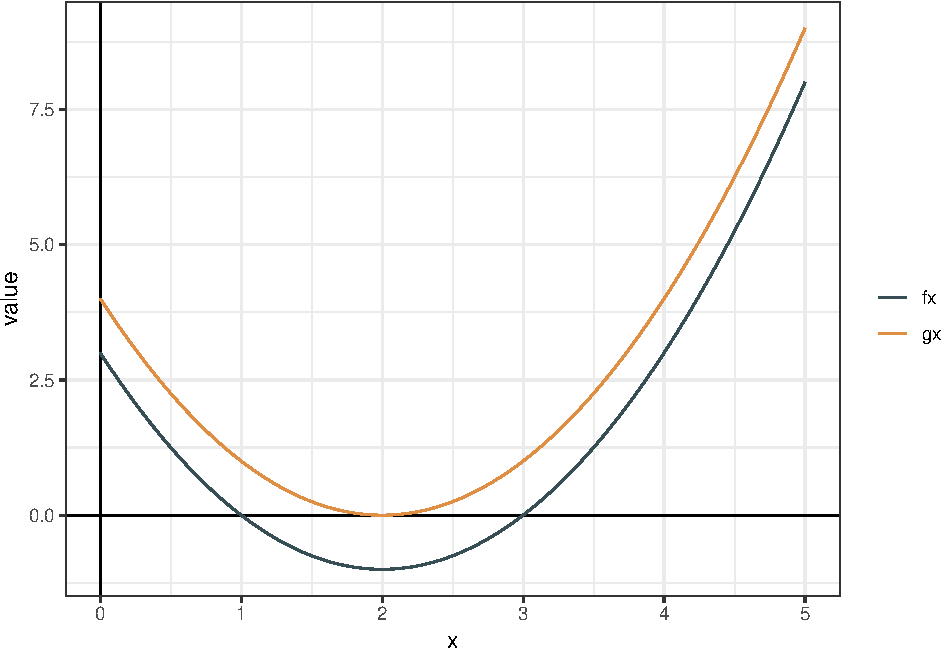
\includegraphics{Glósur_MogT_files/figure-latex/unnamed-chunk-2-1.pdf}

\begin{center}\rule{0.5\linewidth}{\linethickness}\end{center}

\hypertarget{setningin-um-yfirgnfa-samleitni}{%
\section{Setningin um yfirgnæfða samleitni}\label{setningin-um-yfirgnfa-samleitni}}

Látum \((f_n)_{n\geq1}\) vera runu af mælanlegum föllum á málrúmi \((\Omega, \mathcal F, \mu)\) og gerum ráð fyrir að hún stefni n.a. á mælanlegt fall \(f\). Ef til er fall \(g\) úr \(\mathcal L^1(\Omega,\mu)\), sem fullnægir skilyrðinu \(|f_n|\leq g\) fyrir öll \(n\), þá er \(f\in\mathcal L^1(\Omega,\mu)\) og

\[
\int_\Omega fd\mu = \lim_{n\rightarrow\infty}\int_\Omega f_nd\mu.
\]

\begin{center}\rule{0.5\linewidth}{\linethickness}\end{center}

\textbf{Sönnun.} \(\lim_{n\rightarrow\infty}f_n(x) = f(x)\) næstum alls staðar. Látum \(E\) vera mælanlegt mengi með mál 0 þ.a.

\[
\lim_{n\rightarrow\infty}f_n(x) = f(x), \quad \forall x\in \Omega\backslash E
\]

Með því að setja \(f_n = f_n\pi_{\Omega\backslash E}\) og \(f=f\pi_{\Omega\backslash E}\) getum við gert ráð fyrir að \(\lim_{n\rightarrow\infty}f_n(x) = f(x)\). Heildin breytast ekki heldur. Athugum nú að \(|f_n|\leq g\) svo \(f+g\geq0\).

\[
\begin{aligned}
\int_\Omega gd\mu + \int_\Omega fd\mu &= \int_\Omega(g+f)d\mu \\
&= \int_\Omega(g + \liminf f_n)d\mu \\
&\leq \liminf \int_\Omega(g+f_n)d\mu \\
&=\liminf(\int_\Omega gd\mu + \int_\Omega fd\mu) \\
&= \int_\Omega gd\mu + \liminf\int_\Omega f_nd\mu
\end{aligned}
\]

Sjáum að

\[
\begin{aligned}
\int_\Omega fd\mu &\leq \liminf \int_\Omega f_nd\mu 
\end{aligned}
\]

Athugum að \(g - f_n\geq 0\)

\[
\begin{aligned}
\int_\Omega gd\mu - \int_\Omega fd\mu &= \int_\Omega (g - f)d\mu \\
&= \int_\Omega \liminf(g - f_n)d\mu \\
&\leq \liminf(\int_\Omega(g-f_n)d\mu) \\
&= \int_\Omega gd\mu + \liminf(-\int_\Omega f_nd\mu) \\
&= \int_\Omega gd\mu - \limsup\int_\Omega f_nd\mu
\end{aligned}
\]

Sjáum að

\[
\begin{aligned}
\limsup \int_\Omega f_nd\mu &\leq \int_\Omega fd\mu \\
\int_\Omega fd\mu &\leq \liminf\int_\Omega f_nd\mu \\
&\leq \limsup \int_\Omega f_nd\mu \\
&\leq \int_\Omega fd\mu
\end{aligned}
\]

Sv0

\[
\lim_{n\rightarrow\infty}\int_\Omega f_nd\mu = \int_\Omega fd\mu
\]

\begin{center}\rule{0.5\linewidth}{\linethickness}\end{center}

\hypertarget{setning-53}{%
\section{Setning}\label{setning-53}}

Látum \(f\) vera Lebesgue-heildanlegt fall á \(\mathbb R^d\). Þá gildir, fyrir sérhvert \(n\) úr \(\mathbb N^*\), að föllin \(g_n:=f\cdot\mathbf1_{\overline B_{(0,n)}}\) og \(h_n := \min\{f,n\}\) eru heildanleg og

\[
\lim_{n\rightarrow\infty}\int_{\mathbb R^d}|f-g_n|dm = \lim_{n\rightarrow\infty}\int_{\mathbb R^d}|f-h_n|dm = 0.
\]

\begin{center}\rule{0.5\linewidth}{\linethickness}\end{center}

\textbf{Sönnun.} Setjum

\[
g(x) = \sum_{k=1}^\infty |f_k(x)| = \lim_{n\rightarrow\infty}\sum_{k=1}^n|f_k(x)|
\]

þá er \(g\) mælanlegt, \(g(x) \in [0,\infty]\) og \(0\leq g_1\leq g_2 \leq \dots\) og \(g_n\rightarrow g\). Setningin um einhalla samleitni segir

\[
\begin{aligned}
\int_\Omega gd\mu &= \lim_{n\rightarrow\infty} \int_\Omega g_nd\mu \\
&= \lim\int_\Omega\sum_{k=1}^n|f_n|d\mu \\
&= \lim\sum_{k=1}^n\int_\Omega|f_k|d\mu \\
&= \sum_{k=1}^\infty\int_\Omega|f_k|d\mu
\end{aligned}
\]

því er \(g\in\mathcal L^1(\Omega,\mu)\) og \(E=g^{-1}(\infty)\) hefur mál 0. Svo

\[
\sum_{k=1}^\infty|f_k(x)| < \infty, \quad \forall x\in\Omega\backslash E
\]

Svo

\[
\sum_{k=1}^\infty f_n(x) \text{ samleitin, } \quad \forall x\in\Omega\backslash E \\
f(x) = 
\begin{cases}
\sum_{k=1}^\infty f_n(x), x\in\Omega\backslash E,\\
0, x\in E
\end{cases}
\]

Svo

\[
|\sum_{k=1}^\infty f_n(x)| \leq g(x), \quad \forall x\in\Omega \\
\lim_{n\rightarrow\infty}\sum_{k=1}^\infty f_n(x) = f(x) \text{, fyrir næstum öll }x
\]

Svo \(f\in\mathcal L^1(\Omega,\mu)\) og

\[
\int_\Omega fd\mu = \int_\Omega (\lim h_n)d\mu = \lim\int_\Omega h_nd\mu = \lim\int_\Omega \sum_{k=1}^n f_nd\mu = \lim\sum_{k=1}^n\int_\Omega f_nd\mu = \sum_{k=1}^\infty\int_\Omega f_kd\mu
\]

\begin{center}\rule{0.5\linewidth}{\linethickness}\end{center}

\hypertarget{setning-beppo-levi}{%
\section{Setning {[}Beppo Levi{]}}\label{setning-beppo-levi}}

Látum \((f_k)_{k\geq 1}\) vera runu af mælanlegum föllum á málrúmi \((\Omega,\mathcal F,\mu)\) og gerum ráð fyrir að

\[
\sum_{k=1}^\infty\int_\Omega |f_k|d\mu < \infty.
\]

Þá er röðin \(\sum_{k=1}^\infty f_k\) samleitin næstum alls staðar að heildanlegu falli \(f\) á \(\Omega\) og ennfremur gildir

\[
\int_\Omega fd\mu = \sum_{k=1}^\infty \int_\Omega f_kd\mu
\]

\begin{center}\rule{0.5\linewidth}{\linethickness}\end{center}

\textbf{Sönnun.}

\begin{center}\rule{0.5\linewidth}{\linethickness}\end{center}

\hypertarget{vikubla-7}{%
\chapter*{Vikublað 7}\label{vikubla-7}}
\addcontentsline{toc}{chapter}{Vikublað 7}

\hypertarget{dmi-1-4}{%
\section*{Dæmi 1}\label{dmi-1-4}}
\addcontentsline{toc}{section}{Dæmi 1}

Látum \((\Omega, \mathcal F, \mu)\) vera málrúm og \(f, g:\Omega \rightarrow \overline{\mathbb R}\) vera mælanleg föll.

\hypertarget{a-ef-f-og-g-taka-gildi-sin-i--infty-infty-a-gildir}{%
\subsubsection*{\texorpdfstring{(a) Ef \(f\) og \(g\) taka gildi sín í \((-\infty, \infty]\), þá gildir}{(a) Ef f og g taka gildi sín í (-\textbackslash{}infty, \textbackslash{}infty{]}, þá gildir}}\label{a-ef-f-og-g-taka-gildi-sin-i--infty-infty-a-gildir}}
\addcontentsline{toc}{subsubsection}{(a) Ef \(f\) og \(g\) taka gildi sín í \((-\infty, \infty]\), þá gildir}

\[
\text{ess}\sup(f + g) \leq \text{ess}\sup f + \text{ess}\sup g.
\]

\hypertarget{b-ef-f-og-g-taka-gildi-sin-i--infty-infty-a-gildir}{%
\subsubsection*{\texorpdfstring{(b) Ef \(f\) og \(g\) taka gildi sín í \([-\infty, \infty)\), þá gildir}{(b) Ef f og g taka gildi sín í {[}-\textbackslash{}infty, \textbackslash{}infty), þá gildir}}\label{b-ef-f-og-g-taka-gildi-sin-i--infty-infty-a-gildir}}
\addcontentsline{toc}{subsubsection}{(b) Ef \(f\) og \(g\) taka gildi sín í \([-\infty, \infty)\), þá gildir}

\[
\text{ess}\inf f + \text{ess}\inf g \leq \text{ess} \inf(f + g)
\]

\textbf{Ritháttur.} Látum \(\Omega\) vera mengi og \(\mathcal F\) vera safn hlutmengja í \(\Omega\). Þá la´tum við \(\mathcal F^\sigma\) tákna \(\sigma\)-algebruna sem \(\mathcal F\) framleiðir.

Ef \(\Omega'\) er annað mengi, \(f:\Omega \rightarrow \Omega'\) er vörpun og \(\mathcal G\) er safn hlutmengja í \(\Omega'\), þá setjum við

\[
f^{-1}(\mathcal G) := \{f^{-1}(E) | E \in \mathcal G\}.
\]

\begin{center}\rule{0.5\linewidth}{\linethickness}\end{center}

\hypertarget{dmi-2-4}{%
\section*{Dæmi 2}\label{dmi-2-4}}
\addcontentsline{toc}{section}{Dæmi 2}

Látum \(f: \Omega_1 \rightarrow \Omega_2\) vera vörpun milli tveggja mengja. Sannið eftirfarandi fullyrðingar:

\hypertarget{a-ef-mathcal-g-er-sigma-algebra-a-omega_2-a-er-f-1mathcal-g-sigma-algebra-a-omega_1.}{%
\subsubsection*{\texorpdfstring{(a) Ef \(\mathcal G\) er \(\sigma\)-algebra á \(\Omega_2\), þá er \(f^{-1}(\mathcal G)\) \(\sigma\)-algebra á \(\Omega_1\).}{(a) Ef \textbackslash{}mathcal G er \textbackslash{}sigma-algebra á \textbackslash{}Omega\_2, þá er f\^{}\{-1\}(\textbackslash{}mathcal G) \textbackslash{}sigma-algebra á \textbackslash{}Omega\_1.}}\label{a-ef-mathcal-g-er-sigma-algebra-a-omega_2-a-er-f-1mathcal-g-sigma-algebra-a-omega_1.}}
\addcontentsline{toc}{subsubsection}{(a) Ef \(\mathcal G\) er \(\sigma\)-algebra á \(\Omega_2\), þá er \(f^{-1}(\mathcal G)\) \(\sigma\)-algebra á \(\Omega_1\).}

\begin{itemize}
\item
  Þar sem að \(f^{-1}(\emptyset) = \emptyset\) er \(\emptyset\in f^{-1}(\mathcal G)\).
\item
  Ef \(E \in f^{-1}(\mathcal G)\) þá er til \(U \in \mathcal G\) þ.a. \(f^{-1}(U) = E\). Þar sem \(\mathcal G\) er \(\sigma\)-algebra er þá \(U^c\in \mathcal G\), svo við fáum \(f^{-1}(U^c) = E^c\) svo \(E^c \in f^{-1}(\mathcal G)\).
\item
  Tökum þá loks runu \((E_n)_{n\geq1}\) af mengjum í \(f^{-1}(\mathcal G)\). Þá er til samsvarandi runa \((U_n)_{n\geq1}\) í \(\mathcal G\) þ.a. \(f^{-1}(U_n) = E_n\) fyrir öll \(n\). Tökum eftir því að \(\mathcal G\) er \(\sigma\)-algebra og því er \(\bigcup_{n=1}^\infty U_n \in \mathcal G\). Þar sem frummynd falls dreifist yfir sammengi fáum við að \(f^{-1}(\bigcup_{n=1}^\infty U_n) = \bigcup_{n=1}^\infty E_n\) svo \(\bigcup_{n=1}^\infty E_n \in f^{-1}(\mathcal G)\).
\end{itemize}

Ofantalin atriði sýna að \(f^{-1}(\mathcal G)\) sé \(\sigma\)-algebra.

\hypertarget{b-ef-mathcal-f-er-sigma-algebra-a-omega_1-a-er-mathcal-g-esubseteq-omega_2-f-1ein-mathcal-f-sigma-algebra-a-omega_2}{%
\subsubsection*{\texorpdfstring{(b) Ef \(\mathcal F\) er \(\sigma\)-algebra á \(\Omega_1\) þá er \(\mathcal G := \{E\subseteq \Omega_2 | f^{-1}(E)\in \mathcal F\}\) \(\sigma\)-algebra á \(\Omega_2\)}{(b) Ef \textbackslash{}mathcal F er \textbackslash{}sigma-algebra á \textbackslash{}Omega\_1 þá er \textbackslash{}mathcal G := \textbackslash{}\{E\textbackslash{}subseteq \textbackslash{}Omega\_2 \textbar{} f\^{}\{-1\}(E)\textbackslash{}in \textbackslash{}mathcal F\textbackslash{}\} \textbackslash{}sigma-algebra á \textbackslash{}Omega\_2}}\label{b-ef-mathcal-f-er-sigma-algebra-a-omega_1-a-er-mathcal-g-esubseteq-omega_2-f-1ein-mathcal-f-sigma-algebra-a-omega_2}}
\addcontentsline{toc}{subsubsection}{(b) Ef \(\mathcal F\) er \(\sigma\)-algebra á \(\Omega_1\) þá er \(\mathcal G := \{E\subseteq \Omega_2 | f^{-1}(E)\in \mathcal F\}\) \(\sigma\)-algebra á \(\Omega_2\)}

\begin{itemize}
\item
  Þar sem frummynd \(\emptyset\) er ávallt \(\emptyset\) og \(\emptyset\in\mathcal F\) fæst að \(\emptyset \in \mathcal G\).
\item
  Ef \(E \in \mathcal G\) þá er tilsamsvarandi \(U\in \mathcal F\) þ.a. \(f^{-1}(U) = E\). Þar sem \(\mathcal F\) er \(\sigma\)-algebra er \(U^c\in\mathcal F\) og því \(f^{-1}(U^c) = E^c \in \mathcal G\).
\item
  Tökum runu \((E_n)_{n\geq1}\) af mengjum í \(\mathcal G\). Til er samsvarandi runa \((U_n)_{n\geq1}\) af mengjum í \(\mathcal F\) þ.a. \(f^{-1}(U_n) = E_n\) fyrir öll \(n\). Þar sem \(\mathcal F\) sé \(\sigma\)-algebra gildir \(\bigcup_{n=1}^\infty U_n \in \mathcal F\) og þar sem frummynd dreifist yfir sammengi sjáum við að \(f^{-1}(\bigcup_{n=1}^\infty U_n) = \bigcup_{n=1}^\infty E_n\) svo \(\bigcup_{n=1}^\infty\in\mathcal G\).
\end{itemize}

Ofantalin atriði séna að \(\mathcal G\) sé \(\sigma\)-algebra.

\hypertarget{c-ef-mathcal-g-er-safn-af-hlutmengjum-i-omega_2-a-er-f-1mathcal-gsigma-f-1mathcal-gsigma}{%
\subsubsection*{\texorpdfstring{(c) Ef \(\mathcal G\) er safn af hlutmengjum í \(\Omega_2\), þá er \((f^{-1}(\mathcal G))^\sigma = f^{-1}(\mathcal G^\sigma)\)}{(c) Ef \textbackslash{}mathcal G er safn af hlutmengjum í \textbackslash{}Omega\_2, þá er (f\^{}\{-1\}(\textbackslash{}mathcal G))\^{}\textbackslash{}sigma = f\^{}\{-1\}(\textbackslash{}mathcal G\^{}\textbackslash{}sigma)}}\label{c-ef-mathcal-g-er-safn-af-hlutmengjum-i-omega_2-a-er-f-1mathcal-gsigma-f-1mathcal-gsigma}}
\addcontentsline{toc}{subsubsection}{(c) Ef \(\mathcal G\) er safn af hlutmengjum í \(\Omega_2\), þá er \((f^{-1}(\mathcal G))^\sigma = f^{-1}(\mathcal G^\sigma)\)}

Samkvæmt \emph{(a)} er \(f^{-1}(\mathcal G^\sigma)\) \(\sigma\)-algebra sem inniheldur nauðsynlega \(f^{-1}(\mathcal G)\). því fæst að \((f^{-1}(\mathcal G))^\sigma \subseteq f^{-1}(\mathcal G^\sigma)\), svo okkur dugir að leiða út hlutmengjamerkið í öfuga átt. Nú gefur \emph{(b)} að

\[
\mathcal H := \left\{E\subseteq \Omega_2 | f^{-1}(E)\in(f^{-1}(\mathcal G))^\sigma\right\}
\]

sé \(\sigma\)-algebra í \(\Omega_2\). Ef við tökum \(U\in\mathcal G\) þá er \(f^{-1}(U)\in f^{-1}(\mathcal G)\) og þá sér í lagi í \((f^{-1}(\mathcal G))^\sigma\). Því fæst að \(\mathcal G \subseteq \mathcal H\), en þar sem \(\mathcal H\) er \(\sigma\)-algebra er \(\mathcal G^\sigma \subseteq \mathcal H\). Þar sem hlutmengjavensl varðveitast yfir frummyndir er þá \(f^{-1}(\mathcal G^\sigma) \subseteq f^{-1}(\mathcal H) \subseteq (f^{-1}(\mathcal G))^\sigma\).

\begin{center}\rule{0.5\linewidth}{\linethickness}\end{center}

\hypertarget{skilgreining-23}{%
\section*{Skilgreining}\label{skilgreining-23}}
\addcontentsline{toc}{section}{Skilgreining}

Látum \((\Omega_1, \mathcal F)\) og \((\Omega_2, \mathcal G)\) vera tvö mælanleg rúm. Við segjum að vörpun \(\varphi: \Omega_1 \rightarrow \Omega_2\) sé \textbf{mælanleg} ef \(\varphi^{-1}(E) \in \mathcal F\) fyrir öll \(E\in\mathcal G\)

\hypertarget{dmi-3-4}{%
\section*{Dæmi 3}\label{dmi-3-4}}
\addcontentsline{toc}{section}{Dæmi 3}

Látum \((\Omega, \mathcal F)\) vera mælanlegt rúm og \(f\) vera tvinngilt fall á \(\Omega\). Sýnið að fallið \(f\) sé mælanlegt þá og því aðeins að \(f\) sé mælanleg vörpun frá \((\Omega, \mathcal F)\) til \((\mathbb C, \mathcal B)\), þar sem \(\mathcal B\) táknar samkvæmt venju Borel-algebruna á \(\mathbb C\).

\hypertarget{dmi-4-4}{%
\section*{Dæmi 4}\label{dmi-4-4}}
\addcontentsline{toc}{section}{Dæmi 4}

Sýnið að samskeyting endanlega margra mælanlegra varpana sé mælanleg vörpun.

\hypertarget{dmi-5-4}{%
\section*{Dæmi 5}\label{dmi-5-4}}
\addcontentsline{toc}{section}{Dæmi 5}

Látum \((\Omega_1, \mathcal F)\) og \((\Omega_2, \mathcal G)\) vera mælanleg rúm og \(\varphi: \Omega_1 \rightarrow \Omega_2\) vera mælanlega vörpun. Sýnið að fyrir sérhvert mál \(\mu: \mathcal F \rightarrow [0, \infty]\) gildi að fallið

\[
\varphi_* \mu: \mathcal G \rightarrow [0, \infty], \quad E \rightarrow \mu(\varphi^{-1}(E))
\]

sé mál. Við segjum að það sé \textbf{mynd vörpunarinnar} \(\varphi\) \textbf{af málinu} \(\mu\).

\begin{center}\rule{0.5\linewidth}{\linethickness}\end{center}

\begin{itemize}
\item
  \(\varphi_*\mu(\emptyset) = \mu(\varphi^{-1}(\emptyset)) = \mu(\emptyset) = 0\).
\item
  Tökum runu \((E_n)_{n\geq1}\) af innbyrðis sundurlægum mengjum í \(\mathcal G\). Þar sem frummynd dreifist yfir sammengi fæst
\end{itemize}

\[
\mu\left(\varphi^{-1}\left(\bigcup_{n=1}^\infty E_n\right)\right) =
\mu\left(\bigcup_{n=1}^\infty\varphi^{-1}\left( E_n\right)\right) = 
\sum_{n=1}^\infty\mu(\varphi^{-1}(E_n)) = \sum_{n=1}^\infty\varphi_*\mu(E_n).
\]

Ofangreind atriði sýna að \(\varphi_*\mu\) er mál.

\begin{center}\rule{0.5\linewidth}{\linethickness}\end{center}

\hypertarget{dmi-6-4}{%
\section*{Dæmi 6}\label{dmi-6-4}}
\addcontentsline{toc}{section}{Dæmi 6}

Látum \((s_n)_{n\geq1}\) og \(f\) vera eins og í \emph{setningu 12.2.4 og sönnun hennar} og gerum ennfremur ráð fyrir að \(f\) sé \emph{takmarkað} fall. Sýnið að runan \((s_n)_{n\geq1}\) stefni á \(f\) í jöfnum mæli á \(\Omega\).

\begin{center}\rule{0.5\linewidth}{\linethickness}\end{center}

\textbf{Lausn.} Þar sem \(f\) er takmarkað er til \(M\) þ.a. \(||f||<M\). Gefum okkur \(\varepsilon > 0\). Við viljum sýna að til sé \(N\in\mathbb N\) þ.a. \(||f-s_n||_\Omega < \varepsilon\) fyrir öll \(n\geq N\). Við erum búin að sanna að \(s_n \leq f\) fyrir öll \(n\) svo við þurfum í raun bara að sýna að \(f-s_N < \varepsilon\). Fáum nú:

\[
\begin{aligned}
f - s_N &= f - n\mathbf 1_{f^{-1}([n,\infty])} - \sum_{i=1}^{n2^n}\frac{i-1}{2^n}\mathbf1_{f^{-1}([\frac{i-1}{2^n}, \frac{i}{2^n}])} \\
&< (||f|| - n)\mathbf 1_{f^{-1}([n,\infty])} + \sum_{i=1}^{n2^n}(\frac{i}{2^n} - \frac{i-1}{2^n})\mathbf1_{f^{-1}([\frac{i-1}{2^n}, \frac{i}{2^n}])} \\
&< (M - n)\mathbf 1_{f^{-1}([n,\infty])} - \sum_{i=1}^{n2^n}\frac{1}{2^n}\mathbf1_{f^{-1}([\frac{i-1}{2^n}, \frac{i}{2^n}])} \\
&= (M - n)\mathbf 1_{f^{-1}([n,\infty])} - \frac{1}{2^n}\mathbf1_{f^{-1}([0,n])}
\end{aligned}
\]

þar sem síðasta jafnaðarmerkið er vegna þess að summan er yfir kenniföll sundurlægra mengja. Þegar \(n > M\) fæst að \(\mathbf 1_{f^{-1}([n,\infty])} = 0\) og ljóst er að \(\frac{1}{2^n}\mathbf1_{f^{-1}([0,n])}\leq1\) svo við fáum að fyrir nógu stór \(N\) sé \(f-s_N < 2^{-N}\) en þá er ljóst að \(f-s_N < \varepsilon\) fyri rnógu stór \(N\).

\begin{center}\rule{0.5\linewidth}{\linethickness}\end{center}

\hypertarget{dmi-7-3}{%
\section*{Dæmi 7}\label{dmi-7-3}}
\addcontentsline{toc}{section}{Dæmi 7}

Látum \((\Omega, \mathcal F, \mu)\) vera málrúm og \(t = \sum_{k=1}^mb_k\mathbf 1_{E_k}\) vera (ekki endilega staðlaða framsetningu) á einföldu falli á \(\Omega\), þar sem \(E_k \in \mathcal F\) fyrir öll \(k\). Sýnið að

\[
\int_\Omega t d\mu = \sum_{k=1}^m b_k\mu(E_k)
\]

\begin{center}\rule{0.5\linewidth}{\linethickness}\end{center}

\textbf{Lausn.}

\begin{center}\rule{0.5\linewidth}{\linethickness}\end{center}

\hypertarget{dmi-8-1}{%
\section*{Dæmi 8}\label{dmi-8-1}}
\addcontentsline{toc}{section}{Dæmi 8}

Látum \(s\) og \(t\) vera einföld föll á málrúmi. Sýnið að föllin \(\min\{s, t\}\) og \(\max\{s, t\}\) séu líka einföld föll.

\begin{center}\rule{0.5\linewidth}{\linethickness}\end{center}

\textbf{Lausn.}

\begin{center}\rule{0.5\linewidth}{\linethickness}\end{center}

\hypertarget{dmi-9-1}{%
\section*{Dæmi 9}\label{dmi-9-1}}
\addcontentsline{toc}{section}{Dæmi 9}

Látum \(f: \mathbb N \rightarrow [0, \infty]\). Sýnið að fallið \(f\) sé mælanlegt á \((\mathbb N, \mathcal P(\mathbb N), \mu)\) þar sem \(\mu\) er talningarmálið, og um öll hlutmengi E í \(\mathbb N\) gildi

\[
\int_E f d\mu = \sum_{n\in E}f(n).
\]

\begin{center}\rule{0.5\linewidth}{\linethickness}\end{center}

\textbf{Lausn.}

\begin{center}\rule{0.5\linewidth}{\linethickness}\end{center}

\hypertarget{dmi-10}{%
\section*{Dæmi 10}\label{dmi-10}}
\addcontentsline{toc}{section}{Dæmi 10}

Bíl er ekið frá stað A til staðar B á 50 km meðalhraða, en fjarlægðin frá A til B er 25 km. Hann leggur af stað milli kl 12 og 13 (sama dag) og nemur staðar þegar hann kemur til B. Skilgreinum hendingu (slembibreytu, slembistærð) X á líkindarúminu \(([0, 1], P)\), þar sem P táknar einskorðun Lebesgue-málsins við \([0, 1]\), með því að setja

\[
X(t) := \text{ Fjarlægð bílsins frá B kl 13 ef hann leggur af stað kl 12 + t}.
\]

Finnið líkindamálið \(P_X\), sem hendingin X ákvarðar.

\begin{center}\rule{0.5\linewidth}{\linethickness}\end{center}

\textbf{Lausn.}

Sjáum að \(X\) varpar \([0,\frac12]\) í \(0\). Hins vegar fyir \([\frac12,1]\) varpar \(X\) gildinu \(t\) í \(25 - 50t\). Því er \(X(t) = \max(0, 25 - 50t)\). Ljóst er því að frummynd 0 hafi mál \(\frac12\), frummynd alls utan \([0,1]\) sé tóm, og allt í \(]0,1]\) þjappast um helming við að frummynd sé tekin. Því fæst

\[
P_X(B) = \frac12 m(B\cap]0,1]) + 
\begin{cases}
\frac12 \text{ ef } 0 \in B \\
0 \text{ annars}
\end{cases}
\]

\hypertarget{lebesgue-heildi-og-riemann-heildi}{%
\chapter{Lebesgue-heildi og Riemann-heildi}\label{lebesgue-heildi-og-riemann-heildi}}

\hypertarget{dmi-varu}{%
\section{Dæmi (Varúð!)}\label{dmi-varu}}

\[
f:[0, 1] \rightarrow \mathbb R, 
\begin{cases} 
f(x) = 1, x\in\mathbb R\backslash\mathbb Q, \\ 
0, x\in\mathbb Q
\end{cases}
\]

\(\mathbb Q\cap[0,1]\) er núllmengi og einskorðun \(f\) við \([0,1]\backslash[0,1]\cap\mathbb Q\) er fastafallið 1. Hins vegar er fallið ekki Riemann-heildanlegt enda er það ósamfellt í öllum pkt. úr \([0,1]\).

\hypertarget{setning-54}{%
\section{Setning}\label{setning-54}}

Látum \(B\) vera lokaðan (takmarkaðan) kassa í \(\mathbb R^d\). Takmarkað fall \(f:B\rightarrow\mathbb R\) er Riemann-heildanlegt þá og því aðeins að það sé samfelst næstum alls staðar (þ.e.a.s. mengi þeirra punkta þar sem \(f\) er ósamfellt hefur mál núll). Sé svo þá er \(f\) Lebesgue-mælanlegt og Riemann-heildi þess er jafnt Lebesgue-heildinu.

\begin{center}\rule{0.5\linewidth}{\linethickness}\end{center}

\textbf{Sönnun.} Látum \(f: B\rightarrow \mathbb R\) vera takmarkað fall og \(E\) vera mengi allra ósamfellupunkta þess. Fyrir sérhvert \(m\) látum við \(B = C_1^m\cup\dots\cup C_{l_m}^m\) vera skiptingu á \(B\) þ.a. skipting nr. \(m+1\) sé fínni en skipting nr. \(m\) og þ.a. \(\text{diam}(C_j^m)\leq\frac1m\). Setjum \(M_j^m:=\sup_{x\in C_j^m}f(x)\) og \(m_j^m:= \inf_{x\in C_j^m}\). Setjum svo \(t_n:= \sum_{j=1}^{l_m}M_j^m\mathbf1_{C_j^m}\) og \(s_m := \sum_{j=1}^{l_m}m_j^m\mathbf1_{C_j^m}\). Þá fæst \(s_1\leq s_2\leq \dots\leq f \leq \dots \leq t_2 \leq t_1\). Ljóst er að sérhvert tröppufallá B er Lebesgue-heildanlegt og Riemann-heildi þess er jafnt Lebesgue-heildinu.

Nú er \(f\) takmarkað svo að föllin \(s:=\lim_{m\rightarrow\infty} s_m\) og \(t:=\lim_{m\rightarrow\infty}t_m\) eru í \(\mathcal L^1(B,m)\) og \(\int_B sdm = \lim_{m\rightarrow\infty}\int_B s_mdm\), \(\int_Btdm = \lim_{n\rightarrow\infty}\int_B t_mdm\) skv setn um yfirgnæfða samleitni.

Ennfremur gildir að \(s\leq f\leq t\) og \(t(x) = s(x)\) ef \(\omicron(f,x)=0\).

\begin{itemize}
\item
  G.r.f. að \(m(E) = 0\). Þá er \(s(x) = f(x) =t(x)\) f.öll \(x\in B\backslash E\) svo að \(f\) er Lebesgue-mælanlegt skv. setn 11.1.2 vegna þess að \((\mathbb R^d, \mathcal M, m)\) er fullkomið málrúm. Þar eð \(f\) er takmarrkað þá e rþað Lebesgue-heildanlegt og \(\int_B sdm = \int_B fdm = \int_B tdm\), en það hefur í för með sér að \(f\) er Riemann-heildanlegt og jafnframt að \(\int_B fdm\) er Riemann-heildi \(f\) yfir B.
\item
  Öfugt. G.r.f. að \(f\) sé Riemann-heildanlegt og sýnum að \(m(E) = 0\). Við getum valið skiptingarnar þannig að \(\int_B sdm = \int_B tdm\) \emph{(gildir reyndar sjálfkrafa)}. Skv. vikublaði 8 gildir að \(E = \{x\in B | \omicron(f,x)>0\}\) og f.~sérhv. \(\varepsilon>0\) og \(E_\varepsilon = \{x\in B | \omicron(f,x)\geq \varepsilon\}\) er lokað f.öll \(\varepsilon > 0\). Þar eð \(E = E_1\cup E_{\frac12} \cup\dots\) þá nægir að sýna að \(m(E_{\frac1n}) = 0\) f.öll \(m\in\mathbb N^*\). Látum n vera gefið og tökum \(\varepsilon > 0\). Þá er til \(k\) svo stórt að \(\int_B t_kdm - \int_B s_kdm < \frac\varepsilon m\). Tökum eftir að \(B\backslash\bigcup_{j=1}^{l_k}\text{int}(C_j^k)\) er núllmengi svo að \(m(E_{\frac1m}) = m(E_{\frac1m}\cap(\bigcup_{j=1}^{l_k}\text{int}(C_j^k))\). En fyrir \(x\) úr \(\text{int}(C_j^m)\) gildir að \(t_k(x) - s_k(x) \geq \omicron(f,x)\) svo við fáum:
\end{itemize}

\[
\frac1m m(E_{\frac1m}) = \int_{E_{\frac1m}}\frac1mdm = \int_{E_{\frac1m} = m(E_{\frac1m}\cap(\bigcup_{j=1}^{l_k}\text{int}(C_j^k)}\frac1mdm \leq \int_{E_{\frac1m} = m(E_{\frac1m}\cap(\bigcup_{j=1}^{l_k}\text{int}(C_j^k)}(t_k - s_k)dm \leq \int_B t_kdm - \int_B s_kdm < \frac\varepsilon m, \text{ og því } \\
m(E_{\frac1m}) < \varepsilon.
\]

Þar sem \(\varepsilon > 0\) má vera hversu lítið sem vera skal þá er \(m(E_{\frac1m}) = 0\).

\begin{center}\rule{0.5\linewidth}{\linethickness}\end{center}

\hypertarget{setning-55}{%
\section{Setning}\label{setning-55}}

Óeiginlegt Riemann-heildi falls, sem tekur gildi sín í \([0,\infty)\), er samleitið ef og aðeins ef fallið er Lebesgue-heildanlegt og í því tilfelli er Lebesgue-heildið markgildi óeiginlega heildisins.

\begin{center}\rule{0.5\linewidth}{\linethickness}\end{center}

\textbf{Sönnun.} Látum \(A\subseteq\mathbb R^d\) og \(f:A\rightarrow[0,\infty[\). Óeiginlegt Riemann-heildi \(f\) er samleitið ef til er vaxandi runa af Jordan-mælanlegum hlutmengjum \emph{(yfirleitt af sérstakri gerð)} í A sem uppfylla að \(\bigcup A_m = A\) og \(f|_{A_m}\) er Riemann-heildanlegt og \(\lim \int_{A_m}f < \infty\). Við fáum því

\[
\begin{aligned}
\lim_{n\rightarrow\infty}\int_{A_m}f &= \lim_{n\rightarrow\infty}\int_{A_m}fdm \\
&= \lim\int_{\mathbb R^d}f\cdot\mathbf1_{A_m}dm \\
&=  \int_{\mathbb R^d}f\cdot\mathbf1_Adm \\
&= \int_Afdm
\end{aligned}
\]

Sér í lagi fáum við að samleitni Riemann-heildisins er óháð valinu á rununni \((A_m)_{m\geq1}\)

\begin{center}\rule{0.5\linewidth}{\linethickness}\end{center}

\hypertarget{setning-56}{%
\section{Setning}\label{setning-56}}

Látum \(f:[a,b]\rightarrow\mathbb R\) vera samfellt fall. Þá er \(f\) Lebesgue-heildanlegt á \([a,b]\) og fallið

\[
F:[a,b]\rightarrow\mathbb R, \quad x\rightarrow\int_{[a,x]}fdm
\]

er diffranlegt og \(F' = f\).

\begin{center}\rule{0.5\linewidth}{\linethickness}\end{center}

\textbf{Sönnun.}

\begin{center}\rule{0.5\linewidth}{\linethickness}\end{center}

\hypertarget{nalganir-lebesgue-heildanlegra-falla-a-mathbb-rd}{%
\chapter{\texorpdfstring{Nálganir Lebesgue-heildanlegra falla á \(\mathbb R^d\)}{Nálganir Lebesgue-heildanlegra falla á \textbackslash{}mathbb R\^{}d}}\label{nalganir-lebesgue-heildanlegra-falla-a-mathbb-rd}}

\hypertarget{setning-57}{%
\section{Setning}\label{setning-57}}

Látum \(f\) vera Lebesgue-heildanlegt fall á \(\mathbb R^d\) og \(\varepsilon > 0\).

\emph{(i)} Til er kassi \(A\) í \(\mathbb R^d\) og tröppufall \(t:A\rightarrow\mathbb R\), sem uppfyllir

\[
\int_{\mathbb R^d}|f-t|dm < \varepsilon
\]

\emph{(Hér hefur fallið \(t\) verið framlengt með núlli yfir á allt \(\mathbb R^d\)).}

\emph{(ii)} Til er samfellt fall \(g:\mathbb R^d\rightarrow\mathbb R\) og \(d\)-kassi \(C\), sem hafa eftirfarandi eiginleika

\[
\int_{\mathbb R^d}|f-g|dm<\varepsilon \quad \text{og}\quad g(x) = 0, \forall x\in \mathbb R^d\backslash C.
\]

\begin{center}\rule{0.5\linewidth}{\linethickness}\end{center}

\textbf{Sönnun.}

\begin{center}\rule{0.5\linewidth}{\linethickness}\end{center}

\hypertarget{setning-58}{%
\section{Setning}\label{setning-58}}

Látum \(f\) vera í \(\mathcal L^1(\mathbb R,m)\) og setjum, fyrir sérhvert \(k\in\mathbb N\),

\[
s_k:=\int_{-\infty}^\infty f(x) sin(kx)dx \quad \text{og} \quad c_k:=\int_{-\infty}^\infty f(x)cos(kx)dx.
\]

Þá gildir \(\lim_{k\rightarrow\infty}s_k = \lim_{k\rightarrow\infty}c_k=0\).

\begin{center}\rule{0.5\linewidth}{\linethickness}\end{center}

\textbf{Sönnun.}

\begin{center}\rule{0.5\linewidth}{\linethickness}\end{center}

\hypertarget{heildun-me-stikabreytu}{%
\chapter{Heildun með stikabreytu}\label{heildun-me-stikabreytu}}

Í þessari grein táknar \((\Omega, \mathcal F, \mu)\) málrúm og fall \(f:\Omega\times[a,b]\rightarrow\mathbb R\), sem hefur þann eiginleika að

\[
f(-,t):\Omega\rightarrow\mathbb R,\quad x\rightarrow f(x,t)
\]

er mælanlegt fyrir sérhvert \(t\).

\begin{center}\rule{0.5\linewidth}{\linethickness}\end{center}

\hypertarget{setning-59}{%
\section{Setning}\label{setning-59}}

Gerum ráð fyrir að \(f\) fullnægi eftirfarandi skilyrðum

\begin{itemize}
\tightlist
\item
  Til er \(t_0\in[a,b]\), sem hefur þann eiginleika að
\end{itemize}

\[
f(x,t_0) = \lim_{t\rightarrow t_0}f(x,t) \quad \text{fyrir öll }x\in\Omega. 
\]

\begin{itemize}
\tightlist
\item
  Til er \(g\in\mathcal L^1(\Omega,\mu)\) sem uppfyllir
\end{itemize}

\[
|f(x,t)|\leq g(x) \quad \text{fyrir öll } (x,t)\in\Omega\times[a,b].
\]

Þá gildir \(\lim_{t\rightarrow t_0}\int_\Omega f(x,t)d\mu(x) = \int_\Omega f(x,t_0)d\mu(x)\)

\begin{center}\rule{0.5\linewidth}{\linethickness}\end{center}

\textbf{Sönnun.}

\begin{center}\rule{0.5\linewidth}{\linethickness}\end{center}

\hypertarget{setning-60}{%
\section{Setning}\label{setning-60}}

Gerum ráð fyrir að \(f\) fullnægi eftirfarandi skilyrðum:

\begin{itemize}
\item
  Fyrir sérhvert \(x\) úr \(\Omega\) er fallið \(t\rightarrow f(x,t)\) samfellt á \([a,b]\).
\item
  Til er \(g\in\mathcal L^1(\Omega,\mu)\) sem uppfyllir
\end{itemize}

\[
|f(x,t)|\leq g(x) \quad \text{fyrir öll } (x,t)\in\Omega\times[a,b]
\]

Þá gildir að fallið

\[
F:[a,b]\rightarrow\mathbb R,\quad t\rightarrow\int_\Omega f(x,t) d\mu(x)
\]

er samfellt.

\begin{center}\rule{0.5\linewidth}{\linethickness}\end{center}

\textbf{Sönnun.}

\begin{center}\rule{0.5\linewidth}{\linethickness}\end{center}

\hypertarget{setning-61}{%
\section{Setning}\label{setning-61}}

Gerum ráð fyrir að \(f\) fullnægi eftirfarandi skilyrðum:

\begin{itemize}
\item
  Til er \(t_0\in[a,b]\), sem hefur þann eiginleika að \(f(-,t_0)\in\mathcal L^1(\Omega,\mu)\).
\item
  Hlutafleiðan \(\frac{\partial f}{\partial t}\) er til í sérhverjum punkti úr \(\Omega\times[a,b]\).
\item
  Til er \(g\in\mathcal L^1(\Omega,\mu)\) sem uppfyllir
\end{itemize}

\[
\left| \frac{\partial f}{\partial t}(x,t)  \right| \leq g(x) \quad\text{fyrir öll } (x,t)\in\Omega\times[a,b].
\]

Þá gildir að fallið \(F\), sem skilgreint er í \emph{setningu 16.2.2}, er diffranlegt og

\[
\frac{dF}{dt}(t) = \int_\Omega \frac{\partial f}{\partial t}(x,t)d\mu(x).
\]

\begin{center}\rule{0.5\linewidth}{\linethickness}\end{center}

\textbf{Sönnun.}

\begin{center}\rule{0.5\linewidth}{\linethickness}\end{center}

\hypertarget{setning-62}{%
\section{Setning}\label{setning-62}}

Gerum ráð fyrir að \(f\) fullnægi eftirfarandi skilyrðum:

\begin{itemize}
\item
  Fyrir sérhvert \(x\) úr \(\Omega\) er fallið \(t\rightarrow f(x,t)\) samfellt á \([a,b]\).
\item
  Til er \(g\in\mathcal L^2(\Omega,\mu)\) sem uppfyllir
\end{itemize}

\[
|f(x,t)|\leq g(x) \quad \text{fyrir öll }(x,t)\in\Omega\times[a,b].
\]

Þá gildir

\[
\int_a^b\left[\int_\Omega f(x,t)d\mu(x)\right]dt = \int_\Omega\left[\int_a^b f(x,t)dt\right]d\mu(x).
\]

\begin{center}\rule{0.5\linewidth}{\linethickness}\end{center}

\textbf{Sönnun.}

\begin{center}\rule{0.5\linewidth}{\linethickness}\end{center}

\hypertarget{vikubla-8}{%
\chapter*{Vikublað 8}\label{vikubla-8}}
\addcontentsline{toc}{chapter}{Vikublað 8}

\hypertarget{skrimslafri}{%
\chapter{Skrímslafræði}\label{skrimslafri}}

\hypertarget{valfrumsendan}{%
\section{Valfrumsendan}\label{valfrumsendan}}

Látum \((A_i)_{i\in I}\) vera fjölskyldu af hlutmengjum í mengi \(X\), þ.e.a.s. vörpun \(\alpha:I\rightarrow\mathbb P(X)\), og gerum ráð fyrir að mengin séu ekki tóm og innbyrðis sundurlæg. Þá er til vörpun \(f:I\rightarrow X\), sem hefur þann eiginleika að \(f(i)\in A_i\) fyrir sérhvert \(i\) úr \(I\).

\begin{center}\rule{0.5\linewidth}{\linethickness}\end{center}

\hypertarget{setning-63}{%
\section{Setning}\label{setning-63}}

Ekki eru öll hlutmengi í \(\mathbb R\) Lebesgue-mælanleg.

\begin{center}\rule{0.5\linewidth}{\linethickness}\end{center}

\textbf{Sönnun.}

\begin{center}\rule{0.5\linewidth}{\linethickness}\end{center}

\hypertarget{setning-64}{%
\section{Setning}\label{setning-64}}

Ekki eru öll Lebesgue-mælanleg hlutmengi í \(\mathbb R\) Borel-mælanleg.

\begin{center}\rule{0.5\linewidth}{\linethickness}\end{center}

\textbf{Sönnun.}

\begin{center}\rule{0.5\linewidth}{\linethickness}\end{center}

\hypertarget{setning-65}{%
\section{Setning}\label{setning-65}}

Til er Riemann-heildanlegt fall á lokuðu bili í \(\mathbb R\) sem er ekki Borel-mælanlegt.

\begin{center}\rule{0.5\linewidth}{\linethickness}\end{center}

\textbf{Sönnun.}

\begin{center}\rule{0.5\linewidth}{\linethickness}\end{center}

\hypertarget{lp-rum}{%
\chapter{\texorpdfstring{\(L^p\)-rúm}{L\^{}p-rúm}}\label{lp-rum}}

Í þessari grein verður gert ráð fyrir að mælanlegu föllin sem um ræðir séu \emph{tvinngild} nema annað sé tekið fram.

\hypertarget{upprifjun}{%
\section*{Upprifjun}\label{upprifjun}}
\addcontentsline{toc}{section}{Upprifjun}

Látum \(V\) vera vigurrúm (yfir \(\mathbb R\) eða \(\mathbb C\)). Við segjum að raungilt fann \(N\) á \(V\) sé \textbf{norm} eða \textbf{staðall} á V, ef það uppfyllir eftirfarandi skilyrði:

\begin{enumerate}
\def\labelenumi{\arabic{enumi}.}
\tightlist
\item
  \(N(v) \geq 0\) fyrir öll \(v\) úr \(V\)
\item
  \(N(v) = 0\) þá og því aðeins að \(v = 0\)
\item
  \(N(cv) = |c|N(v)\) fyrir öll \(v\) úr \(V\) og allar tölur \(c\)
\item
  \(N(u + v) \leq N(u) + N(v)\) fyrir öll \(u\) og \(v\) úr \(V\)
\end{enumerate}

Sé skilyrði \emph{2.} sleppt kallsat N \textbf{hálfnorm} eða \textbf{hálfstaðall}.

\begin{center}\rule{0.5\linewidth}{\linethickness}\end{center}

\hypertarget{setning-66}{%
\section*{Setning}\label{setning-66}}
\addcontentsline{toc}{section}{Setning}

Látum \((\Omega,\mathcal F, \mu)\) vera málrúm. Þá gerir venjuleg samlagning falla og margföldun þeirra með tölu mengið \(\mathcal L^1(\Omega,\mu)\) að \(\mathbb C\)-vigurrúmi og fallið

\[
N_\mu: \mathcal L^1(\Omega,\mu)\rightarrow\mathbb R, \quad f\rightarrow\int_\Omega|f|d\mu
\]

er hálfnorm.

\begin{center}\rule{0.5\linewidth}{\linethickness}\end{center}

\textbf{Sönnun.}

\begin{enumerate}
\def\labelenumi{\arabic{enumi}.}
\tightlist
\item
  \(|f| \geq 0\) svo \(\int_\Omega |f|d\mu \geq 0\)
\item
  \(\int_\Omega |cf|d\mu = |c| \int_\Omega |f|d\mu\)
\item
  \(|f+g| \leq |f| + |g|\) svo \(\int_\Omega |f + g|d\mu \leq \int_\Omega|f|d\mu + \int_\Omega|g|d\mu\)
\end{enumerate}

\begin{center}\rule{0.5\linewidth}{\linethickness}\end{center}

Skilgreinum vensl á \(\mathcal L^1(\Omega,\mu)\) með því að segja að \(f\) sé \(\mu\)\textbf{-jafngilt} \(g\), táknað \(f\sim_\mu g\), ef \(f\) og \(g\) eru eins næstum alls staðar m.t.t. \(\mu\).

\hypertarget{fing-2}{%
\section*{Æfing}\label{fing-2}}
\addcontentsline{toc}{section}{Æfing}

Sýnið að \(\sim_\mu\) séu jafngildisvensl á \(\mathcal L^1(\Omega,\mu)\).

\begin{center}\rule{0.5\linewidth}{\linethickness}\end{center}

\textbf{Lausn.}

\begin{enumerate}
\def\labelenumi{\arabic{enumi}.}
\tightlist
\item
  \(f \sim_\mu f\) þar sem \(f=f\) alls staðar.
\item
  Ef \(f\sim_\mu g\) þá er \(f=g\) næstum alls staðar og sömuleiðis \(g=f\) svo \(g\sim_\mu f\)
\item
  Ef \(f=g\) á mengi \(F_1\in \Omega\) þ.a. \(\mu(\Omega\backslash F_1)=0\) og \(g=h\) á mengi \(F_2\in\Omega\) þ.a. \(\mu(\Omega\backslash F_2)=0\) er \(f=h\) á menginu \(F_1\cap F_2\) og \(\mu(\Omega\backslash(F_1\cap F_2)) = 0\).
\end{enumerate}

\begin{center}\rule{0.5\linewidth}{\linethickness}\end{center}

Setjum \(L^1(\Omega,\mu) := \mathcal L^1(\Omega,\mu)\backslash\sim_\mu\) og táknum jafngildisflokk falls \(f\) úr \(\mathcal L^1(\Omega,\mu)\) með \([f]\).

\hypertarget{setning-67}{%
\section*{Setning}\label{setning-67}}
\addcontentsline{toc}{section}{Setning}

Aðgerðirnar \(c[f]:=[cf]\) og \([f] + [g] := [f + g]\) eru vel skilgreindar á \(L^1(\Omega,\mu)\) og gera \(L^1(\Omega,\mu)\) að vigurrúmi. Jafnframt er fallið

\[
||\cdot||_1: L^1(\Omega,\mu)\rightarrow\mathbb R,\quad[f]\rightarrow||[f]||_1:=\int_\Omega|f|d\mu
\]

vel skilgreint norm.

\begin{center}\rule{0.5\linewidth}{\linethickness}\end{center}

Við munum iðulega leyfa okkur að skrifa \(||f||_1\) í stað \(||[f]||_1\).

\hypertarget{uppfrifjun}{%
\section*{Uppfrifjun}\label{uppfrifjun}}
\addcontentsline{toc}{section}{Uppfrifjun}

Látum \(a\) og \(b\) vera úr \([-\infty,\infty]\). Raungilt fall \(\varphi\) á opna bilinu \((a,b)\) er sagt \textbf{kúpt} ef um öll \(x,y\in(a,b)\) og öll \(\lambda\in[0,1]\) gildir

\[
\varphi[(1-\lambda)x + \lambda y] \leq (1 - \lambda)\varphi(x) + \lambda\varphi(y).
\]

\hypertarget{fing-3}{%
\section*{Æfing}\label{fing-3}}
\addcontentsline{toc}{section}{Æfing}

Látum \(a,b\in[-\infty,\infty]\). Sannið eftirfarandi fullyrðingar.

\begin{enumerate}
\def\labelenumi{\arabic{enumi}.}
\tightlist
\item
  Fall \(\varphi:(a,b)\rightarrow\mathbb R\) er kúpt þá og því aðeins að um allar rauntölur \(s,t\) og \(u\), sem uppfylla \(a<s<t<u<b\), gildi
\end{enumerate}

\[
\frac{\varphi(t) - \varphi(s)}{t - s} \leq \frac{\varphi(u) - \varphi(t)}{u - t}.
\]

\begin{enumerate}
\def\labelenumi{\arabic{enumi}.}
\setcounter{enumi}{1}
\item
  Diffranlegt fall á \((a,b)\) er kúpt þá og því aðeins að afleiða þess sé vaxandi á \((a,b)\).
\item
  Öll kúpt föll á \((a,b)\) eru samfelld á \((a,b)\).
\end{enumerate}

\begin{center}\rule{0.5\linewidth}{\linethickness}\end{center}

\textbf{Lausn.}

\begin{center}\rule{0.5\linewidth}{\linethickness}\end{center}

\hypertarget{setning-ojafna-jensens}{%
\section*{Setning (Ójafna Jensens)}\label{setning-ojafna-jensens}}
\addcontentsline{toc}{section}{Setning (Ójafna Jensens)}

Látum \((\Omega,\mathcal F,\mu)\) vera málrúm sem uppfyllir \(\mu(\Omega)=1\), þ.e. líkindarúm. Látum \(a,b\in[-\infty,\infty]\) og \(f:\Omega\rightarrow(a,b)\) vera heildanleft fall. Þá gildir um sérhvert kúpt fall \(\varphi\) á \((a,b)\) að

\[
\varphi\left(\int_\Omega fd\mu\right) \leq \int_\Omega (\varphi\circ f)d\mu.
\]

\begin{center}\rule{0.5\linewidth}{\linethickness}\end{center}

\textbf{Sönnun.}

\begin{center}\rule{0.5\linewidth}{\linethickness}\end{center}

\hypertarget{setning-ojofnur-holders-og-minkowski}{%
\section*{Setning (Ójöfnur Hölders og Minkowski)}\label{setning-ojofnur-holders-og-minkowski}}
\addcontentsline{toc}{section}{Setning (Ójöfnur Hölders og Minkowski)}

Látum \((\Omega,\mathcal F,\mu)\) vera málrúm og \(p\) og \(q\) vera tölur úr \((1,\infty)\) sem uppfylla \(\frac1p + \frac1q = 1\). Um öll mælanleg föll \(f,g:\Omega\rightarrow[0,\infty]\) gilda þá jöfnurnar:

\begin{enumerate}
\def\labelenumi{\arabic{enumi}.}
\item
\end{enumerate}

\[
\int_\Omega fgd\mu \leq \left(\int_\Omega f^pd\mu\right)^{\frac1p}\left(\int_\Omega g^qd\mu\right)^{\frac1q}
\]

og

\begin{enumerate}
\def\labelenumi{\arabic{enumi}.}
\setcounter{enumi}{1}
\item
\end{enumerate}

\[
\left(\int_\Omega (f+g)^pd\mu\right)^\frac1p \leq
\left(\int_\Omega f^pd\mu\right)^{\frac1p} +
\left(\int_\Omega g^pd\mu\right)^{\frac1p}
\]

Fyrri ójafnan er kennd við \textbf{Hölder} og sú síðari við \textbf{Minkowski}.

\begin{center}\rule{0.5\linewidth}{\linethickness}\end{center}

\textbf{Sönnun.} Sönnum fyrst hjálparsetningu: Ef x og y eru jákvæðar rauntölurog \(\alpha,\beta\in(0,1)\) þ.a. \(\alpha+\beta=1\) gildir

\[
x^\alpha y^\beta\leq \alpha x + \beta y
\]

x = 0 er augljóts. Látum x \textgreater{} 0 og skoðum \(f(t) = (1 - \beta) + \beta t - t^\beta\) fyrir \(t\geq0\). Við höfum \(f'(t) = \beta - \beta t^{\beta-1} = \beta(1 - t^{\beta-1})\) og þar sem \(0<\beta<1\) er \(f'(t) < 0\) á \((0,1)\) og \(f'(t) > 0 á (1, \infty)\). Höfum því að \(f\) er minnkandi á \([0,1]\) en vaxandi á \([1, \infty)\). \(f(1) = 0\) er því eina lágildi \(f\) á \([0,\infty)\), svo \(f(t)\geq0\) fyrir \(t\geq0\). Setjum nú \(t=\frac yx\). Þá gildir \((1 - \beta) + \beta\frac yx - (\frac yx)^\beta \geq 0\), það er \((\frac yx)^\beta \leq\alpha + \beta \frac yx\). Með því að skrifa \(x=x^{\alpha+\beta}\) fáum við að \(x^{\alpha+\beta}(\frac yx)^\beta\leq\alpha x + \beta x\frac yx\), svo að \(x^\alpha y^\beta \leq \alpha x + \beta y\).

\begin{enumerate}
\def\labelenumi{\arabic{enumi}.}
\tightlist
\item
  Ójafna Hölders:
\end{enumerate}

\textbf{Skref 1.} Gerum ráð fyrir að \(\Vert f\Vert_p = \Vert g\Vert_q = 1\). Þurfum að sýna að \(\Vert fg\Vert_1\leq1\). Notum hjálparsetninguna að ofan með \(\alpha =\frac1p\), \(\beta = \frac1q\), \(x=\vert f\vert^p\), \(y = \vert g\vert^q\), og fáum

\[
\vert fg\vert = x^{\frac1p}y^{\frac1q} \leq \frac1p\vert f\vert^p + \frac1q\vert g\vert^q.
\]

Með því að heilda fáum við

\[
\int_\Omega\vert fg\vert d\mu\leq\frac1p\int_\Omega\vert f\vert^pd\mu + \frac1q\int_\Omega\vert g\vert^qd\mu = \frac1p + \frac1q = 1.
\]

\textbf{Skref 2.} Fyrir almenn \(f\in L^p\) og \(g\in L^q\) ritum við \(\Vert f\Vert_p = a\) og \(\Vert g\Vert_q = b\). Skilgreinum svo föllin \(\tilde f = \frac1a f\) og \(\tilde g = \frac1bg\). Þau uppfylla forsendur skrefs 1 að ofan svo \(\Vert\tilde f\tilde g\Vert_1\leq\Vert\tilde f\Vert_p\Vert\tilde g\Vert_q\), sem leiðir að

\[
\frac{1}{ab}\Vert fg\vert_1 \leq \frac1a\Vert f\Vert_p\frac1b\Vert g\Vert_q
\]

Margföldun með \(ab\) klárar svo sönnun.

\begin{enumerate}
\def\labelenumi{\arabic{enumi}.}
\setcounter{enumi}{1}
\tightlist
\item
  Ójafna Minkowski
\end{enumerate}

Gerum ráð fyrir að \(1 < p < \infty\). Höfum

\[
\vert f + g\vert^p =\vert(f + g)(f + g)^{p-1}\vert\leq\vert f\vert\vert f + g\vert^{p-1} + \vert g\vert\vert f + g\vert^{p - 1}.
\]

Með því að velja \(q\) þannig að \(\frac1p + \frac1q = 1\), það er \(p + q = pq\), fáum við

\[
\vert f + g\vert^{(p-1)q} = \vert f + g\vert^p < \infty.
\]

Því er \((f + g)^{p-1}\in L^q\) og

\[
\Vert(f+g)^{p-1}\Vert_q = \left(\int_\Omega\vert f + g\vert^p d\mu \right)^{\frac1q}.
\]

Beitum ójöfnu Hölders:

\[
\begin{aligned}
\int_\Omega\vert f + g\vert^p d\mu &\leq 
\int_\Omega\vert f\vert\vert f + g\vert^{p-1}d\mu + \int_\Omega\vert g\vert\vert f + g\vert^{p-1}d\mu \\
&\leq \left(\int_\Omega \vert f\vert^pd\mu\right)^{\frac1p}\left(\int_\Omega\vert f + g\vert^pd\mu\right)^{\frac 1q}
+ \left(\int_\Omega \vert g\vert^pd\mu\right)^{\frac1p}\left(\int_\Omega\vert f + g\vert^pd\mu\right)^{\frac 1q} \\
&= A\left(\left(\int_\Omega\vert f\vert^pd\mu   \right)^{\frac1p} + \left(\int_\Omega\vert g\vert^pd\mu\right)^{\frac1p}\right),
\end{aligned}
\]

þar sem \(A = \left(\int_\Omega\vert f + g\vert^pd\mu\right)^{\frac1q}\). Ef \(A=0\) þá er \(\Vert f + g\Vert_p = 0\) og ekkert sem þarf að sanna. Gerum því ráð fyrir að \(A>0\) og deilum með \(A\):

\[
\begin{aligned}
\Vert f + g\Vert_p &= \left(\int_\Omega\vert f + g\vert^pd\mu\right)^{1 - \frac1q} \\
&= \frac1A\left(\int_\Omega\vert f + g\vert^pd\mu\right) \\
&\leq \left(\int_\Omega\vert f\vert^pd\mu\right)^{\frac1p} + \left(\int_\Omega\vert g\vert^pd\mu\right)^{\frac1p} \\
&= \Vert f\Vert_p + \Vert g\Vert_p.
\end{aligned}
\]

\begin{center}\rule{0.5\linewidth}{\linethickness}\end{center}

Við skilgreinum jafngildisvenslin \(\sim_\mu\) eins og áður: \(f\sim_\mu g\) þá og því aðeins að \(f - g\) sé núll næstum alls staðar.

Fyrir sérhvert \(p\in[1,\infty)\) látum við \(\mathcal L^p(\Omega,\mu)\) tákna mengi allra (tvinngildra) mælanlegra falla á \(\Omega\), sem hafa þann eiginleika að \(f^p\) er í \(\mathcal L^1(\Omega,\mu)\) og setjum

\[
L^p(\Omega,\mu) := \mathcal L^p(\Omega,\mu)/\sim_\mu.
\]

Jafngildisflokkur falls \(f\) úr \(L^p(\Omega,\mu)\) verður táknaður \([f]\)

\hypertarget{upprifjun-1}{%
\section*{Upprifjun}\label{upprifjun-1}}
\addcontentsline{toc}{section}{Upprifjun}

Fyrir fall \(h:\Omega\rightarrow[-\infty,\infty]\) segjum við að

\[
\text{ess}\sup h := \inf\{c|h\leq c \text{ næstum alls staðar}\}
\]

sé \textbf{raunverulegt efra mark} \(h\).

\begin{center}\rule{0.5\linewidth}{\linethickness}\end{center}

\hypertarget{skilgreining-24}{%
\section*{Skilgreining}\label{skilgreining-24}}
\addcontentsline{toc}{section}{Skilgreining}

Við segjum að (tvinngilt) fall \(f\) á \(\Omega\) sé \textbf{raunverulega takmarkað} ef \(\text{ess}\sup|f| < \infty\).

\begin{center}\rule{0.5\linewidth}{\linethickness}\end{center}

Látum \(\mathcal L^\infty(\Omega,\mu)\) tákna mengi allra (tvinngildra) mælanlegra falla á \(\Omega\), sem eru raunverulega takmörkuð og setjum

\[
L^\infty(\Omega,\mu) := \mathcal L^\infty(\Omega,\mu)/\sim_\mu.
\]

Jafngildisflokkur falls \(f\) úr \(L^\infty(\Omega,\mu)\) verður táknaður \([f]\).

\begin{center}\rule{0.5\linewidth}{\linethickness}\end{center}

\hypertarget{setning-68}{%
\section*{Setning}\label{setning-68}}
\addcontentsline{toc}{section}{Setning}

Fyrir sérhvert \(1\leq p \leq \infty\) eru aðgerðirnar \(c[f] := [cf]\) og \([f] + [g] := [f + g]\) vel skilgreindar á \(L^p(\Omega,\mu)\) og gera \(L^p(\Omega,\mu)\) að vigurrúmi. Ennfremur gildir að fallið

\[
||\cdot||_p: L^p(\Omega,\mu) \rightarrow \mathbb R, \quad [f]\rightarrow||[f]||_p:= \left(\int_\Omega|f|^pd\mu\right)^{\frac1p}
\]

er vel skilgreint norm þegar \(1\leq p < \infty\) og fallið

\[
||\cdot||_\infty : L^\infty(\Omega,\mu) \rightarrow \mathbb R, \quad [f]\rightarrow ||[f]||_\infty:=\text{ess}\sup|f|
\]

er vel skilgreint norm.

\begin{center}\rule{0.5\linewidth}{\linethickness}\end{center}

\textbf{Sönnun.}

\begin{center}\rule{0.5\linewidth}{\linethickness}\end{center}

\hypertarget{setning-69}{%
\section*{Setning}\label{setning-69}}
\addcontentsline{toc}{section}{Setning}

Gerum ráð fyrir að \(p\) og \(q\) séu úr \([1,\infty]\) og uppfylli \(\frac1p + \frac1q = 0\). Þá gildir um öll \(f\) úr \(L^p(\Omega,\mu)\) og öll \(g\) úr \(L^q(\Omega,\mu)\) að \(fg\in L^1(\Omega,\mu)\) og

\[
||f||_1 \leq ||f||_p||g||_q.
\]

\begin{center}\rule{0.5\linewidth}{\linethickness}\end{center}

\textbf{Sönnun.}

\begin{center}\rule{0.5\linewidth}{\linethickness}\end{center}

\hypertarget{upprifjun-2}{%
\section*{Upprifjun}\label{upprifjun-2}}
\addcontentsline{toc}{section}{Upprifjun}

Ef \((V, ||\cdot||)\) er staðlað vigurrúm, þá er fallið

\[
d: V\times V \rightarrow [0,\infty), \quad (x,y)\rightarrow||x-y||
\]

firð á \(V\) og við lítum ávallt á \(V\) sem firðrúm með tilliti til þessarar firðar.

Runa \((x_n)_{n\geq1}\) í firðrúmi \((X,d)\) er kölluð \textbf{Cauchy-runa} ef fyrir sérhvert \(\varepsilon > 0\) er til \(N\in\mathbb N\) sem uppfyllir skilyrðið

\[
d(x_n,x_m)<\varepsilon\quad \text{fyrir öll } m,n\geq N.
\]

Við segjum að firðrúmið \((X,d)\) sé \textbf{fullkomið} ef sérhver Cauchy-runa í X er alsamleitin.

Staðlað vigurrúm kallast \textbf{Banach-rúm} ef það er fullkomið (sem firðrúm).

\hypertarget{fingar}{%
\section*{Æfingar}\label{fingar}}
\addcontentsline{toc}{section}{Æfingar}

\begin{enumerate}
\def\labelenumi{\arabic{enumi}.}
\item
  Cauchy-runa sem hefur samleitna hlutrunu er samleitin.
\item
  Hlutrúm í fullkomnu firðrúmi er fullkomið þá og því aðeins að það sé lokað.
\end{enumerate}

\begin{center}\rule{0.5\linewidth}{\linethickness}\end{center}

\textbf{Lausn.}

\begin{center}\rule{0.5\linewidth}{\linethickness}\end{center}

\hypertarget{setning-70}{%
\section*{Setning}\label{setning-70}}
\addcontentsline{toc}{section}{Setning}

Látum \(1 \leq p \leq \infty\) og \((f_n)_{n\geq1}\) vera runu í \(\mathcal L^p(\Omega,\mu)\), sem hefur þann eiginleika að \(([f_n])_{n\geq1}\) er Cauchy-runa í \(L^p(\Omega)\). Þá er til fall \(f\in\mathcal L^p(\Omega)\) og hlutruna \((f_{n_k})_{k\geq1}\) í \((f_n)_{n\geq1}\), sem uppfylla skilyrðið

\[
\lim_{k\rightarrow\infty}f_{n_k}(x) = f(x), \quad \text{fyrir næstum öll } x\in\Omega.
\]

\begin{center}\rule{0.5\linewidth}{\linethickness}\end{center}

\textbf{Sönnun.}

\begin{center}\rule{0.5\linewidth}{\linethickness}\end{center}

\hypertarget{setning-71}{%
\section*{Setning}\label{setning-71}}
\addcontentsline{toc}{section}{Setning}

Firðrúmið \(L^p(\Omega,\mu)\) er fullkomið fyrir sérhvert \(p\) úr \([1,\infty]\).

\begin{center}\rule{0.5\linewidth}{\linethickness}\end{center}

\textbf{Sönnun.}

\begin{center}\rule{0.5\linewidth}{\linethickness}\end{center}

\hypertarget{athugasemd-5}{%
\section*{Athugasemd}\label{athugasemd-5}}
\addcontentsline{toc}{section}{Athugasemd}

Setninguna má einnig orða svo að \((L^p(\Omega,\mu), ||\cdot||_p)\) sé Banach-rúm.

\hypertarget{setning-72}{%
\section*{Setning}\label{setning-72}}
\addcontentsline{toc}{section}{Setning}

Gerum ráð fyrir að \(\mu(\Omega) < \infty\). Þá gildir \(L^q(\Omega,\mu)\subseteq L^p(\Omega, \mu)\) þegar \(1\leq p \leq q \leq \infty\).

\begin{center}\rule{0.5\linewidth}{\linethickness}\end{center}

\textbf{Sönnun.}

\begin{center}\rule{0.5\linewidth}{\linethickness}\end{center}

Við segjum að tvinngilt fall á \(\Omega\) sé \textbf{einfalt} ef það er mælanlegt og tekur bara endanlega mörg gildi.

Látum \(\mathcal S\) tákna vigurrúm allra einfaldra falla \(s\) á \(\Omega\), sem uppfylla skilyrðið

\[
\mu(\{x\in\Omega|s(x)\neq 0\}) < \infty.
\]

Það er hlutrúm í \(L^p(\Omega,\mu)\) fyrir öll \(p\).

\begin{center}\rule{0.5\linewidth}{\linethickness}\end{center}

\hypertarget{setning-73}{%
\section*{Setning}\label{setning-73}}
\addcontentsline{toc}{section}{Setning}

Hlutrúmið \(\mathcal S\) er þétt í \(L^p(\Omega,\mu)\) þegar \(1\leq p< \infty\)

\begin{center}\rule{0.5\linewidth}{\linethickness}\end{center}

\textbf{Sönnun.}

\begin{center}\rule{0.5\linewidth}{\linethickness}\end{center}

\hypertarget{setning-74}{%
\section*{Setning}\label{setning-74}}
\addcontentsline{toc}{section}{Setning}

Látum \(1\leq p < \infty\) og \(f\in\mathcal L^p(\mathbb R^d,m)\). Fyrir sérhvert \(\varepsilon > 0\) er þá til lokað og takmarkað hlutmengi \(K\) í \(\mathbb R^d\) og samfellt fall \(g\), sem er núll fyrir utan \(K\) og uppfyllir \(||f-g||_p < \varepsilon\).

\begin{center}\rule{0.5\linewidth}{\linethickness}\end{center}

\textbf{Sönnun.}

\begin{center}\rule{0.5\linewidth}{\linethickness}\end{center}

\hypertarget{vikubla-9}{%
\chapter*{Vikublað 9}\label{vikubla-9}}
\addcontentsline{toc}{chapter}{Vikublað 9}

\hypertarget{dmi-1-5}{%
\section*{Dæmi 1}\label{dmi-1-5}}
\addcontentsline{toc}{section}{Dæmi 1}

Sýnið að föllin \(f_n = \frac1n\mathbf1_{[0,n]}\) stefni í jöfnum mæli á fallið \(f=0\) á \(\mathbb R\) þegar \(n\rightarrow\infty\) og

\[
\int_\mathbb R fdm \neq \lim_{n\rightarrow\infty}\int_\mathbb R f_ndm.
\]

Hvernig lítur þessi niðurstaða út í ljósi setningar um einhalla samleitni, setningar Fatous og setningar um yfirgnæfða samleitni?

Gerið samskonar úttekt á rununni \((g_n)_{n\geq1}\) þar sem \(g_n := n\mathbf1_{[\frac1n,\frac2n]}\).

\hypertarget{lausn}{%
\subsubsection*{Lausn}\label{lausn}}
\addcontentsline{toc}{subsubsection}{Lausn}

\(\mathbf{f_n.}\) Þar sem \(||f_n||_{\mathbb R} = n^{-1}\) liggur ljóst fyrir að \(f_n\) stefni í jöfnum mæli á \(0\) þegar \(n\rightarrow\infty\). Þar sem \(f_n\) er einfallt fall fæst beint skv. skilgr. að \(\int_{\mathbb R}f_n dm = \frac1n([0,n])=1\). Því er markgildi þessara heilda ljóslega 1. Hins vegar er heildi \(f\) ljóslega \(0\) á \(\mathbb R\). Þar sem runan \((f_n)_{n\geq1}\) er ekki vaxandi þá á reglan um einhalla samleitni ekki við. Setning Fatous gildir, enda er \(0\leq 1\) eins og setningin spáir fyrir um. Til þess að beita setningunni um yfirgnæfða samleitni þyrfti að vera til \(h\) sem yfirgnæfir öll \(f\). Það þyrfti þá að vera jafn a.m.k. \(n^{-1}\) á \([n-1,n]\) fyrir öll \(n>0\). En þetta \(h\) er ekki í \(\mathcal L(\mathbb R,m)\) því summan af \(n^{-1}\) frá \(n=1\) upp í \(\infty\) er ekki samleitin.

\(\mathbf{g_n.}\) Þar sem sérhver punktur \(x\in\mathbb R\) liggur alltaf að lokum (eða alltaf) utan \([n^{-1},2n^{-1}]\) stefnir \(g_n\) á núllfallið. Hins vegar stefnir \(g_n\) ekki á núllfallið í jöfnum mæli því \(||g_n||_{\mathbb R} = n\). Þar sem \(g_n\) er einfalt fall fæst beint skv. skilgr. að \(\int_{\mathbb R}g_ndm = nm([n^{-1},2n^{-1}]) = 1\). Því er markgildi þessara heilda ljóslega 1. Hins vegar er heildi \(g\) ljóslega \(0\) á \(\mathbb R\). Þar sem runan \((g_n)_{n\geq1}\) er ekki vaxandi þá á reglan um einhalla samleitni ekki við. Setning Fatous gildir, enda er \(0\leq1\) eins og setningin spáir fyrir um. Til þess að beita setningunni um yfirgnæfða samleitni þyrfti að vera til \(h\) sem yfirgnæfir öll \(f\). Það þyrfti þá að vera jafn a.m.k \(n\) á \([n^{-1},2n^{-1}]\) fyrir öll \(n>0\). En þetta \(h\) er ekki í \(\mathcal L(\mathbb R,m)\) því summan af 1 frá \(n=1\) upp í \(\infty\) er ekki samleitin.

\begin{center}\rule{0.5\linewidth}{\linethickness}\end{center}

\hypertarget{dmi-2-5}{%
\section*{Dæmi 2}\label{dmi-2-5}}
\addcontentsline{toc}{section}{Dæmi 2}

Sýnið fram á að samfellt og takmarkað fall á Jordan-mælanlegu mengi í \(\mathbb R^d\) sé Riemann-heildanlegt.

\emph{VINSAMLEG ÁBENDING}: Dæmið gengur út á að sanna setningu 4.3.4 í fyrirlestrunum svo þið megið ekki nota hana.

\begin{center}\rule{0.5\linewidth}{\linethickness}\end{center}

\textbf{Lausn.} C, Jordan-mælanlegt mengi

\[
f:C\rightarrow \mathbb R, \quad \tilde f: \mathbb R^d \rightarrow \mathbb R, \text{ framlengt}
\]

Tökum kassa \(R\) þ.a. \(C\subseteq R\). \(\tilde f\) er heildanlegt á \(R\) þá og því aðeins að mengi þeirra punkta þar sem \(f\) er ósamfellt sé núllmengi \emph{(setning 14.2.1)}, en það mengi er innihaldið í \(\partial C\), sem er núllmengi \emph{(dæmi 3.3)}.

\begin{center}\rule{0.5\linewidth}{\linethickness}\end{center}

\hypertarget{dmi-3-5}{%
\section*{Dæmi 3}\label{dmi-3-5}}
\addcontentsline{toc}{section}{Dæmi 3}

Látum \((\Omega,\mathcal F, \mu)\) vera málrúm. Við segjum að fall \(f:\Omega\rightarrow\mathbb C\) sé \textbf{heildanlegt} ef raungildi föllin \(\text{Re}f\) og \(\text{Im}f\) eru bæði heildanleg og þá setjum við

\[
\int_\Omega fd\mu := \int_\Omega \text{Re}fd\mu + i\int_\Omega \text{Im}fd\mu.
\]

Sýnið að tvinngilt fall \(f\) á \(\Omega\) sé heildanlegt þá og því aðeins að fallið \(|f|\) sé heildanlegt á \(\Omega\) og sé svo þá gildi

\[
\left|\int_\Omega fd\mu\right| \leq \int_\Omega |f|d\mu.
\]

\begin{center}\rule{0.5\linewidth}{\linethickness}\end{center}

\textbf{Lausn.}

\begin{center}\rule{0.5\linewidth}{\linethickness}\end{center}

\hypertarget{dmi-4-5}{%
\section*{Dæmi 4}\label{dmi-4-5}}
\addcontentsline{toc}{section}{Dæmi 4}

Látum \(f\) vera stak í \(\mathcal L^1(\mathbb R,m)\) og skilgreinum fall \(\hat f:\mathbb R\rightarrow \mathbb C\) með því að setja

\[
\hat f(u):= \int_\mathbb R e^{iux}f(x)dm
\]

Gerið grein fyrir að fallið \(\hat f\) sé samfellt í jöfnum mæli á \(\mathbb R\).

\begin{center}\rule{0.5\linewidth}{\linethickness}\end{center}

\textbf{Lausn.}

\begin{center}\rule{0.5\linewidth}{\linethickness}\end{center}

\hypertarget{upprifjun-ur-linulegri-algebru}{%
\section*{Upprifjun úr línulegri algebru}\label{upprifjun-ur-linulegri-algebru}}
\addcontentsline{toc}{section}{Upprifjun úr línulegri algebru}

Látum \(e_1, \dots, e_d\) vera venjulega grunninn fyrir \(\mathbb R^d\). Gagntæk línuleg vörpun \(\mathbb R^d\rightarrow\mathbb R^d\) er samskeyting endanlega margra línulegra varpana sem hver um sig ákvarðast af einu eftirfarandi skilyrða:

\begin{itemize}
\item
  \(L(e_i) = e_i\) ef \(i\neq j\), og \(L(e_j) = ae_j\) þar sem \(a\in\mathbb R\).
\item
  \(L(e_i) = e_i\) ef \(i\neq j\), og \(L(e_j) = e_j + e_k\).
\item
  \(L(e_i) = e_i\) ef \(i\not\in \{j,k\}\), og \(L(e_j) = e_k, L(e_k)=e_j\).
\end{itemize}

\hypertarget{dmi-5-5}{%
\section*{Dæmi 5}\label{dmi-5-5}}
\addcontentsline{toc}{section}{Dæmi 5}

Látum \(T:\mathbb R^d\rightarrow\mathbb R^d\) vera línulega vörpun, sem er af einni af þeim þremur gerðum sem lýst er í upprifjuninni hér að ofan, og \(B\) vera tening í \(\mathbb R^d\).

\begin{enumerate}
\def\labelenumi{\arabic{enumi}.}
\item
  Geri grein fyrir að \(T(B)\) sé Lebesgue-mælanlegt mengi.
\item
  Sýnið að
\end{enumerate}

\[
m(T(B)) = |\det(T)||B|.
\]

\emph{Ábendingar}: Sannið fyrst niðurstöðuna fyrir \(B\) þegar núllpunkturinn er einn af hornpunktum \(B\). Skoðið sérstaklega tilfellið \(d=2\) og teiknið skýringamyndir.

\begin{enumerate}
\def\labelenumi{\arabic{enumi}.}
\setcounter{enumi}{2}
\item
  Gerið grein fyrir að \(T\) sé mælanleg vörpun frá \((\mathbb R^d,\mathcal M)\) til \((\mathbb R^d,\mathcal M)\).
\item
  Látum \(T_*m\) tákna mynd vörpunarinnar \(T\) af Lebesgue-málinu \(m\). Sýnið að
\end{enumerate}

\[
T_*m = \frac{1}{|\det T|}m.
\]

\begin{center}\rule{0.5\linewidth}{\linethickness}\end{center}

\textbf{Lausn.}

Athugið: Þríhyrningur í \(\mathbb R^2\) sem hefur tvær hliðar samsíða ásunum er Jordan-mælanlegur vegna þess að

\begin{Shaded}
\begin{Highlighting}[]
\KeywordTok{tibble}\NormalTok{(}\DataTypeTok{x =} \KeywordTok{seq}\NormalTok{(}\DecValTok{0}\NormalTok{, }\DecValTok{1}\NormalTok{, }\FloatTok{0.01}\NormalTok{),}
       \DataTypeTok{y =} \DecValTok{1} \OperatorTok{-}\StringTok{ }\NormalTok{x) }\OperatorTok\StringTok{ }
\StringTok{    }\KeywordTok{ggplot}\NormalTok{(}\KeywordTok{aes}\NormalTok{(x, y)) }\OperatorTok{+}
\StringTok{    }\KeywordTok{geom_line}\NormalTok{()}
\end{Highlighting}
\end{Shaded}

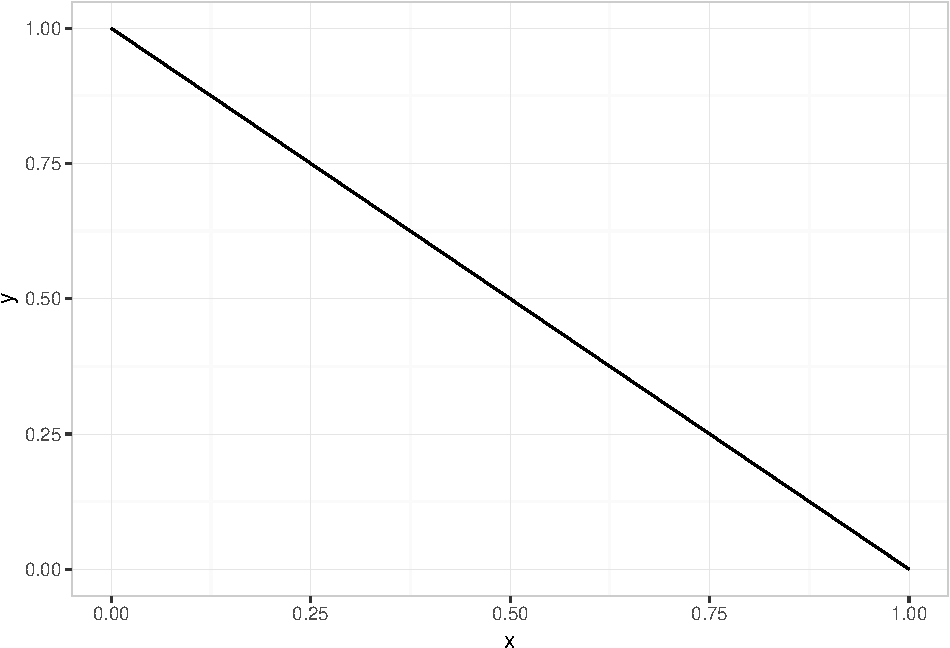
\includegraphics{Glósur_MogT_files/figure-latex/unnamed-chunk-4-1.pdf}

\begin{enumerate}
\def\labelenumi{\arabic{enumi}.}
\tightlist
\item
  \(\alpha)\) \(m(T(B)) = |a|h^{d-1}\) þar sem \(h\) er brúnalengd teningsins. \(T(B)\) er kassi og þar með mælanlegt.
\end{enumerate}

\(\beta)\) Nóg að skoða \(j = 1, k = 2, d = 2\).

\(T(B)\) er sammengi tveggja mælanlegra mengja og þar með

\(\gamma)\). \(T(B) = B\) o.s.fr.

\begin{enumerate}
\def\labelenumi{\arabic{enumi}.}
\setcounter{enumi}{1}
\tightlist
\item
  \(\alpha)\) \(m(T(B)) = |T(B)| = |a|h^d = |\det T||B|\)
\end{enumerate}

\(\beta)\) Ljóst að \(Þ_2 \cup (Þ_1 - e_2) = B\) og því \(m(T(B)) = m(B) = |B| = |\det T||B|\)

\(\gamma)\) Augljóst vegna \(|\det T| = |(-1)| = 1\)

\begin{enumerate}
\def\labelenumi{\arabic{enumi}.}
\setcounter{enumi}{2}
\tightlist
\item
  Ef \(U\) er opið í \(\mathbb R^d\) þá er \(T^{-1}(U)\) opið í \(\mathbb R^d\). Auk þess eru öll opin mengi í \(\mathbb R^d\) af gerðinni \(T^{-1}(u)\) þar sem \(u\) er opið.
\end{enumerate}

Látum \(\mathcal O\) tákna safn allra opinna menngja í \(\mathbb R^d\). Þá er \(\mathcal O^\sigma = \mathcal B\). Skv. ofansögðu er \(T^{-1}(\mathcal O) = \mathcal O\) og skv. dæmi 7.2 er \(T^{-1}(\mathcal O^\sigma) = (T^{-1}(\mathcal O))^\sigma = \mathcal B\).

Munum: Sérhvert opið mengi er teljanlegt sammengi af næstum því innbyrðis sundurlægum teningum.

Sýnum: Ef \(E\) er núllmengi, þá er \(T^{-1}(E)\) núllmengi.

Sö: G.r.f. að \(m(E) = 0\) og gefið sé \(\varepsilon > 0\). Veljum opið mengi \(u\supseteq E\) þ.a. \(m(u)<\varepsilon / |\det T^{-1}|\). Skrifum \(u = \bigcup_{m\geq1}B_m\) þar sem \((B_m)_{m\geq1}\) er runa af næstum innbyrðis sundurlægum kössum. Þá fæst að \(m(u) = \sum_{n\geq1}|B_n|\) og \(T^{-1}(E) \subseteq T^{-1}(u) = \bigcup_{n\geq1}T^{-1}(B_n)\). Af því leiðir að

\[
m^*(T^{-1}(E)) \leq \\
\sum_{n\geq1} m(T^{-1}(B_n)) = \\
\sum_{n\geq1} \frac{1}{|\det T|}|B_n| < \varepsilon
\]

Sýnum nú að \(T:(\mathbb R^d,\mathcal M)\rightarrow (\mathbb R^d,\mathcal M)\) sé mælanlegt. Ef \(E \in\mathcal M\), þá veljum við \(A,C\in\mathcal B\) þ.a. \(A\subseteq E\subseteq C\) og \(m(C\backslash A) = 0\). Þá er \(E = A \cup (E\backslash A)\) og því \(T^{-1}(E) = T^{-1}(A) \cup T^{-1}(E\backslash A)\) mælanlegt.

\begin{enumerate}
\def\labelenumi{\arabic{enumi}.}
\setcounter{enumi}{3}
\tightlist
\item
  Ef \(u\) er opið þá skrifum við \(u = \bigcup_{n\geq1}B_n\) þar sem \(B_n\) eru næstum innbyrðis sundurlægir teningar. Þá er \(u' = \bigcup \text{int}(B_n) \subseteq u\) og \(m(u') = m(u)\). Af því leiðir að
\end{enumerate}

\[
T_*m(u) = m(T^{-1}(u)) = \\ 
m(\bigcup_{n\geq1} T^{-1}(\text{int} B_n)) = \\
\sum_{n\geq1} \frac{1}{|\det T|}|B_n| = \\
\frac{1}{|\det T|}m(u)
\]

Ef \(E\in \mathcal M\) og \(\varepsilon > 0\) þá er \(m(E) = \inf\{m(u) | u\in\mathcal O, E\subseteq u\}\).

\[
T_*m(E) = m(T^{-1}(E)) = \\
\inf\{m(w) | w\in\mathcal O, T^{-1}(E)\subseteq w\} = \\
\inf\{m(T^{-1}(u)) | | u\in \mathcal O, E\subseteq u\} = \\
\frac{1}{|\det T|}\inf\{m(u) | u\in\mathcal O, E\subseteq u\}.v
\]

\begin{center}\rule{0.5\linewidth}{\linethickness}\end{center}

\hypertarget{dmi-6-5}{%
\section*{Dæmi 6}\label{dmi-6-5}}
\addcontentsline{toc}{section}{Dæmi 6}

Látum \(T:\mathbb R^d\rightarrow\mathbb R^d\) vera gagntæka línulega vörpun. Gerið grein fyrir að \(T\) sé mælanleg vörpuframt að

\[
T_*m = \frac{1}{|\det T|}m.
\]

Ályktið út frá því að fyrir sérhvert Lebesgue-mælanlegt mengi \(E\) í \(\mathbb R^d\) og sérhvert \(f\) úr \(\mathcal L^1(E,\mu)\) gildi

\[
\int_E fdm = \int_{T^{-1}(E)}(f\circ T)|\det(T)| dm.
\]

Hvað er hægt að segja um málið \(T_*m\) ef ekki er gert ráð fyrir að T sé gagntæk?

\begin{center}\rule{0.5\linewidth}{\linethickness}\end{center}

\textbf{Lausn.}

\begin{center}\rule{0.5\linewidth}{\linethickness}\end{center}

\hypertarget{dmi-7-4}{%
\section*{Dæmi 7}\label{dmi-7-4}}
\addcontentsline{toc}{section}{Dæmi 7}

Látum \((\Omega,\mathcal F,\mu)\) vera málrúm og \(f:\Omega\rightarrow[0,\infty]\) vera mælanlegt fall sem uppfyllir

\[
0<\int_\Omega fd\mu <\infty.
\]

Sýnið að

\[
\begin{aligned}
\lim_{n\rightarrow\infty}\int_\Omega n\log[1+(f/n)^\alpha]d\mu =
\begin{cases}
\infty &\text{ef } 0<\alpha<1 \\
\int_\Omega fd\mu &\text{ef } \alpha = 1 \\
0 &\text{ef } 1<\alpha<\infty.
\end{cases}
\end{aligned}
\]

\begin{center}\rule{0.5\linewidth}{\linethickness}\end{center}

\textbf{Lausn.}

\emph{Upprifjun:} Notum skilgreininguna á afleiðu til að sýna:

\[
\begin{aligned}
\lim_{t\rightarrow0^+}\frac{kn(1 + at)}{t} &= a, a\in\mathbb R
\end{aligned}
\]

Af því leiðir að \(n^\alpha\ln(1 + \frac{a}{n^\alpha}) = \frac{\ln(1 + a\frac{1}{n^\alpha})}{1/n^\alpha} \rightarrow a\), þegar \(n\rightarrow\infty\) fyrir hvaða \(\alpha\in]0,\infty[\) sem er. Af þessu leiðir að

\[
\lim_{n\rightarrow\infty}n\ln(1 + (\frac an)^\alpha) \\ =\lim_{n\rightarrow\infty}n^{1-\alpha}n^\alpha\ln(1 + \frac{a^\alpha}{n^\alpha}), a\neq 0 \\
= \begin{cases}
0, \alpha > 1\\
a, \alpha = 1 \\
\infty, 0<\alpha<1.
\end{cases}
\]

Setjum \(E = \Omega\backslash f^{-1}(\{0,\infty\})\). Þá er \(\int_E fd\mu = \int_\Omega fd\mu\).

Nú fæst:

\(\alpha < 1\):

\[
\liminf_n\int_\Omega n\log(1 + (\frac fn)^\alpha)d\mu =\\
\liminf_n \int_En\log(1+(\frac fn)^\alpha)d\mu \geq
\int_E\liminf_n n\log(1 + (\frac fn)^\alpha)d\mu = \\
\int_E\infty d \mu = \infty.
\]

\(\alpha = 1\):

Tökum nú eftir að \(\ln(1 + t) \leq t, \forall t>-1\). Við fáum því að

\[
n\ln(1 + (\frac fn)) \leq  f, \forall n
\]

og setning um yfirgnæfða samleitni gefur þá

\[
\lim_n\int_\Omega n\ln(1 + (\frac fn))d\mu = \\
\int_E \lim_n n\ln(1 + (\frac fn))d\mu = \\
\int_E fd\mu = \int_\Omega fd\mu
\]

\(\alpha>1:\) Setjum

\[
g(x) = \frac{\ln(1 + x^\alpha)}{x} \rightarrow 0, x\rightarrow +\infty, 0^+
\]

Svo að til er \(M>0\) þ.a. \(g(x) \leq M, \forall x\). Af því leiðir að

\[
\frac{\ln(1 + (\frac fn)^\alpha)}{f/n} \leq M \rightarrow (f\neq 0) \\
n\ln(1 + (\frac fn)^\alpha) \leq M\cdot f
\]

Setningin um yfirgnæfða samleitni gefur þá:

\[
\lim_n\int_E n\ln(1 + (\frac fn)^\alpha)d\mu = \\
\int_E \lim_n n\ln(1 + (\frac fn)^\alpha)d\mu = \\
\int_E 0 d\mu = 0.
\]

\begin{center}\rule{0.5\linewidth}{\linethickness}\end{center}

\hypertarget{dmi-8-2}{%
\section*{Dæmi 8}\label{dmi-8-2}}
\addcontentsline{toc}{section}{Dæmi 8}

Reiknið heildið

\[
\int_0^1\frac{x^2-1}{\log x}dx
\]

með því að beita setningu 16.2.3 á fallið

\[
F(t) := \int_0^1\frac{x^t-1}{\log x}dx
\]

\begin{center}\rule{0.5\linewidth}{\linethickness}\end{center}

\textbf{Lausn.} Setjum

\[
f(x,t) = \frac{x^1 - t}{\ln x}, (x,t)\in(0,1)\times[0,2].
\]

Þá er

\[
|\frac{\partial f}{\partial t}(x,t)|=x^t \leq 1
\]

sem er tegranlegt yfir bilið frá 0 uppí 1 svo við betum beitt diffrunarsetningu Hermanns til að fá:

\[
F'(t) = \int_0^1 \frac{\partial}{\partial t}\frac{x^t - 1}{\ln x}dx =\\
\int_0^1x^tdx = \\
\frac{1}{1+t}.
\]

En þá er

\[
\int_0^1 \frac{x^2 - 1}{\ln x}dx = \\
F(2) = \\
\int_0^2 F'(2)dt + F(0) = \\
\ln 3
\]

\begin{center}\rule{0.5\linewidth}{\linethickness}\end{center}

\hypertarget{dmi-9-2}{%
\section*{Dæmi 9}\label{dmi-9-2}}
\addcontentsline{toc}{section}{Dæmi 9}

Sérhverja tölu \(x\in[0,1]\) er hægt að rita á nákvæmlega einn veg sem tvíundabrot \(x=0,a_1a_2\dots\) samkvæmt viðteknum venjum. Sýnið að fyrir sérhvert \(n\geq 1\) sé fallið

\[
[0,1] \rightarrow\mathbb R, \quad x\rightarrow a_n
\]

mælanlegt.

\begin{center}\rule{0.5\linewidth}{\linethickness}\end{center}

\textbf{Lausn.} Nóg að sýna að \(a_n:[0,1]\rightarrow\mathbb R, \quad x\rightarrow a_n(x)\) sé þ.a. \(a_n^{-1}(0)\) sé mælanlegt. En þetta er bersýnilega sammengi af bilum. Bwahahaha!!

\begin{center}\rule{0.5\linewidth}{\linethickness}\end{center}

\hypertarget{innfeldisrum}{%
\chapter{Innfeldisrúm}\label{innfeldisrum}}

\hypertarget{upprifjun-3}{%
\section*{Upprifjun}\label{upprifjun-3}}
\addcontentsline{toc}{section}{Upprifjun}

Látum \(V\) vera \(\mathbb K\)-vigurrúm (\(\mathbb K\) annað hvort \(\mathbb R\) eða \(\mathbb C\)). \textbf{Innfeldi} á \(V\) er fall

\[
\langle \cdot,\cdot \rangle:V\times V\rightarrow\mathbb K
\]

sem uppfyllir eftirtalin skilyrði

\begin{enumerate}
\def\labelenumi{\arabic{enumi}.}
\tightlist
\item
  \(\langle x,x \rangle > 0\) ef \(x\neq 0\)
\item
  \(\langle x,y \rangle = \overline{\langle y,x \rangle}\).
\item
  \(\langle x + y,z \rangle = \langle x,y \rangle + \langle y,z \rangle\)
\item
  \(\langle cx,y \rangle = c\langle x,y \rangle\) fyrir allar tölur \(c\).
\end{enumerate}

Vigurrúm með gefnu innfeldi er nefnt \textbf{infeldisrúm}.

\begin{center}\rule{0.5\linewidth}{\linethickness}\end{center}

\hypertarget{setning-75}{%
\section*{Setning}\label{setning-75}}
\addcontentsline{toc}{section}{Setning}

Látum \(V\) vera innfeldisrúm og setjum \(||x|| := \sqrt{\langle x,x \rangle}\) fyrir öll \(x\) úr \(V\). Þá gildir um öll \(x\) og \(y\) úr \(V\):

\begin{enumerate}
\def\labelenumi{\arabic{enumi}.}
\tightlist
\item
  \(|\langle x,y \rangle| \leq ||x|| ||y||\)
\item
  \(||x + y|| \leq ||x|| + ||y||\).
\end{enumerate}

Fyrri ójafnan er kennd við Cauchy, Búnjakovskí og Schwartz, en sú síðari kallast þríhyrningsójafnan.

\begin{center}\rule{0.5\linewidth}{\linethickness}\end{center}

\textbf{Sönnun.}

\begin{center}\rule{0.5\linewidth}{\linethickness}\end{center}

Af ofangreindri setningu leiðir að fyrir sérhvert innfeldisrúm \(V\) er fallið \(V\rightarrow\mathbb R, x\rightarrow||x||\) norm á \(V\). Við köllum það \textbf{innfeldisnormið} á \(V\).

Innfeldisrúm er kallað \textbf{Hilbert-rúm} ef það er fullkomið m.t.t. firðarinnar sem innfeldisnormið gefur af sér.

\begin{center}\rule{0.5\linewidth}{\linethickness}\end{center}

\hypertarget{setning-76}{%
\section*{Setning}\label{setning-76}}
\addcontentsline{toc}{section}{Setning}

Fyrir \(f\) og \(g\) úr \(L^2(\Omega,\mu)\) setjum við

\[
\langle f,g \rangle := \int_\Omega f\bar g d\mu.
\]

Þá er \(\langle \cdot,\cdot \rangle\) innfeldi á \(L^2(\Omega,\mu)\) sem gefur af sér normið \(||\cdot||_2\) og gerir \(L^2(\Omega,\mu)\) að Hilbert-rúmi.

\begin{center}\rule{0.5\linewidth}{\linethickness}\end{center}

\textbf{Sönnun.} Sýnum að \(L^2(\Omega,\mu)\) sé vigurrúm.

Setjum \(f,g\in L^2(\Omega,\mu)\). Þar sem \(\vert f(x) + g(x) \vert \leq 2\max(\vert f(x)\vert, \vert g(x)\vert)\) höfum við að

\[
\vert f(x) + g(x)\vert^2\leq4(\vert f(x)\vert^2 + \vert g(x)\vert^2),
\]

og því

\[
\int_\Omega \vert f + g\vert^2d\mu \leq 4\int_\Omega\vert f\vert^2d\mu + 4\int_\Omega\vert g\vert^2d\mu < \infty
\]

svo að \(f + g\in L^2(\Omega, \mu)\). Augljóst er að ef \(a\in \mathbb R\) þá er \(af\in L^2(\Omega,\mu)\). Því er \(L^2(\Omega,\mu)\) vigurrúm.

Sýnum svo að innfeldið sé vel skilgreint, þ.e. að \(f\bar g\in L^2(\Omega, \mu)\).

Rifjum upp að fyrir \(A,B\geq0\) gildir \(2AB\leq A^2 + B^2\) svo að

\[
\int_\Omega f\bar gd\mu \leq \frac12 (\Vert f\Vert^2 + \Vert g\Vert^2).
\]

Sýnum að innfeldið uppfylli skilyrðin fjögur.

\begin{enumerate}
\def\labelenumi{\arabic{enumi}.}
\tightlist
\item
  \(\langle f, f\rangle = \int_\Omega |f|^2d\mu \geq 0\)
\item
  \(\langle f, g\rangle = \int_\Omega f\bar gd\mu = \overline{\int_\Omega \bar fgd\mu} = \overline{\langle g, f\rangle}\)
\item
  \(\langle f + h, g \rangle = \int_\Omega(f + h)\bar gd\mu = \int_\Omega f\bar gd\mu + \int_\Omega h\bar gd\mu = \langle f, g\rangle + \langle h, g\rangle\)
\item
  \(\langle af, g\rangle = \int_\Omega af\bar gd\mu = a\int_\Omega f\bar hd\mu = a\langle f,g\rangle\)
\end{enumerate}

Sýnum svo að \(L^2(\Omega,\mu)\) sé fullkomið í innfeldisnorminu.

Látum \((f_n)_{n\geq1}\) vera Cauchy runu í \(L^2\), og skoðum hlutrunu hennar, \((f_{n_k})_{k\geq1}\), sem hefur þá eiginleika að

\[
\Vert f_{n_{k+1}} - f_{n_k}\Vert_2 \leq 2^{-k}, \quad \text{fyrir öll }k\geq 1.
\]

Setjum nú

\[
g_k = \sum_{i=1}^k \Vert f_{n_{i+1}} - f_{n_i}\Vert_2, \quad g= \lim_{k\rightarrow\infty}g_k = \sum_{i=1}^\infty\Vert f_{n_{i+1}} - f_{n_i}\Vert_2.
\]

Þríhyrningsójafnan gefur okkur að \(\Vert g_k\Vert_2 \leq \sum_{i=1}^k2^{-i}\) og við beitum reglu Fatou á jákvæðu mælanlegu föllum \(g_k^2\) þannig að

\[
\Vert g\Vert^2_2 = \int_\Omega \lim_{k\rightarrow\infty} g_k^2d\mu \leq \liminf_{k\rightarrow\infty}\int_\Omega g_k^2d\mu\leq 1.
\]

Við sjáum að \(g\) er endanlegt næstum alls staðar og \(f_{n_1} + \sum_{i\geq1}(f_{n_{i+1}} - f_{n_i})\) er alsamleitin næstum alls staðar með markgildi \(f\). Við þurfum nú að sýna að \(f\in L^2\). Tökum fyrst eftir að \(f = \lim_{k\rightarrow\infty}f_{n_k}\) næstum alls staðar, og fyrir gefið \(\varepsilon > 0\) getum við fundið \(N\) svo að \(\Vert f_n - f_m\Vert_2 < \varepsilon\) fyrir sérhver \(m,n\geq N\). Beitum reglu Fatou á rununa \((\vert f_{n_i} - f_m\vert^2)_{i\geq1}\) og látum \(i\rightarrow \infty\). Fáum

\[
\int_\Omega \vert f - f_m \vert d\mu \leq \liminf_{i\rightarrow\infty}\int_\Omega\vert f_{n_i} - f_m\vert^2d\mu \leq \varepsilon^2.
\]

Fáum því að \(f - f_m\in L^2\) og þá \(f = f_m + (f - f_m) \in L^2\) auk þess að \(\Vert f - f_m\Vert_2 < \varepsilon\) fyrir öll \(m\geq N\). Því gildir að \(f_m\rightarrow f\) í innfeldisnorminu svo að \(L^2(\Omega,\mu)\) er fullkomið.

\begin{center}\rule{0.5\linewidth}{\linethickness}\end{center}

\hypertarget{setning-77}{%
\section*{Setning}\label{setning-77}}
\addcontentsline{toc}{section}{Setning}

Látum \(V\) vera innfeldisrúm og \(v\in V\). Þá eru föllin \(x\rightarrow \langle x,v\rangle\), \(x\rightarrow \langle v,x\rangle\) og \(x\rightarrow ||x||\) samfelld á \(V\).

\begin{center}\rule{0.5\linewidth}{\linethickness}\end{center}

\textbf{Sönnun.}

\begin{center}\rule{0.5\linewidth}{\linethickness}\end{center}

\hypertarget{setning-78}{%
\section*{Setning}\label{setning-78}}
\addcontentsline{toc}{section}{Setning}

Látum \(V\) vera innfeldisrúm. Þá gildir um öll \(x\) og \(y\) úr \(V\):

\begin{enumerate}
\def\labelenumi{\arabic{enumi}.}
\tightlist
\item
  \(||x + y||^2 + ||x - y||^2 = 2(||x|| + ||y||)\).
\item
  \(4\langle x,y\rangle = ||x+y||^2 - ||x-y||^2 + i(||x+iy||^2 - ||x-iy||^2)\).
\end{enumerate}

Fyrri jafnan er kölluð \emph{samsíðungsregla} og sú síðari \emph{skautunarjafna}.

\begin{center}\rule{0.5\linewidth}{\linethickness}\end{center}

\textbf{Sönnun.}

\begin{center}\rule{0.5\linewidth}{\linethickness}\end{center}

\hypertarget{skilgreining-25}{%
\section*{Skilgreining}\label{skilgreining-25}}
\addcontentsline{toc}{section}{Skilgreining}

Við segjum að tveir vigrar \(x\) og \(y\) úr innfeldisrúmi séu \textbf{þverstæðir} eða \textbf{hornréttir} (hvor á annan) ef \(\langle x,y\rangle = 0\). Þetta er stundum táknað \(x\perp y\).

Látum \(X\) vera hlutmengi í innfeldisrúmi \(V\). Setjum

\[
X^\perp := \{v\in V|\langle v,x\rangle = 0, \forall x\in X\}
\]

og köllum \(X^\perp\) \textbf{hornrétt fyllirúm} \(X\).

Fljótséð er að \(X^\perp\) er lokað hlutvigurrúm í \(V\).

\hypertarget{fing-4}{%
\section*{Æfing}\label{fing-4}}
\addcontentsline{toc}{section}{Æfing}

Látum \(x\) og \(y\) vera þverstæða vigra í innfeldisrúmi. Sýnið að

\[
||x||^2 + ||y||^2 = ||x + y||^2.
\]

\begin{center}\rule{0.5\linewidth}{\linethickness}\end{center}

\textbf{Lausn.}

\begin{center}\rule{0.5\linewidth}{\linethickness}\end{center}

\hypertarget{setning-79}{%
\section*{Setning}\label{setning-79}}
\addcontentsline{toc}{section}{Setning}

Látum \(K\) vera lokað hlutrúm í Hilbert-rúmi \(H\) og \(x\in H\). Þá er til nákvæmlega einn vigur \(y\) úr \(K\), sem fullnægir eftirfarandi jafngildum skilyrðum.

\begin{enumerate}
\def\labelenumi{\arabic{enumi}.}
\tightlist
\item
  \(x - y\in K^\perp\)
\item
  \(||x - y|| = \inf\{||x - z|| | z \in K\}\).
\end{enumerate}

\begin{center}\rule{0.5\linewidth}{\linethickness}\end{center}

\textbf{Sönnun.}

\begin{center}\rule{0.5\linewidth}{\linethickness}\end{center}

\hypertarget{setning-80}{%
\section*{Setning}\label{setning-80}}
\addcontentsline{toc}{section}{Setning}

Látum \(K\) vera lokað hlutrúm í Hilbert-rúmi H. Þá er hægt að skrifa sérhvern vigur \(x\) úr \(K\) á nákvæmlega einn veg sem \(x = x_1 + x_2\) þar sem \(x_1 \in K\) og \(x_2 \in K^\perp\). Auk þess gildir að varpanirnar

\[
P:H\rightarrow H, x\rightarrow x_1 \quad \text{og} \quad Q:H\rightarrow H, x\rightarrow x_2
\]

eru línulegar og fullnægja skilyrðinu

\[
\Vert x\Vert^2 = \Vert P(x)\Vert^2 + \Vert Q(x)\Vert^2, \quad \text{fyrir öll }x\in H.
\]

\begin{center}\rule{0.5\linewidth}{\linethickness}\end{center}

Sönnun.

\begin{center}\rule{0.5\linewidth}{\linethickness}\end{center}

\hypertarget{skilgreining-26}{%
\section*{Skilgreining}\label{skilgreining-26}}
\addcontentsline{toc}{section}{Skilgreining}

Varpanirnar \(P\) og \(Q\) kallast \textbf{hornrétt ofanvörp} á \(K\) og \(K^\perp\).

\hypertarget{skilgreining-27}{%
\section*{Skilgreining}\label{skilgreining-27}}
\addcontentsline{toc}{section}{Skilgreining}

Línuleg vörpun af \(\mathbb K\)-vigurrúmi yfir í \(\mathbb K\) kallast \textbf{línulegt felli} (á vigurrúminu).

\hypertarget{setning-81}{%
\section*{Setning}\label{setning-81}}
\addcontentsline{toc}{section}{Setning}

Látum \(L\) vera \emph{samfellt línulegt felli} á Hilbert-rúmi \(H\). Þá er til nákvæmlega einn vigur \(y\) úr \(H\), sem uppfyllir skilyrðið

\[
L(x) = \langle x,y\rangle, \quad \text{fyrir öll }x\in H.
\]

\begin{center}\rule{0.5\linewidth}{\linethickness}\end{center}

\textbf{Sönnun.}

\begin{center}\rule{0.5\linewidth}{\linethickness}\end{center}

\hypertarget{vikubla-10}{%
\chapter*{Vikublað 10}\label{vikubla-10}}
\addcontentsline{toc}{chapter}{Vikublað 10}

\hypertarget{dmi-1-skil}{%
\section*{Dæmi 1 (Skil)}\label{dmi-1-skil}}
\addcontentsline{toc}{section}{Dæmi 1 (Skil)}

Reiknið heildið

\[
\int_0^{\frac\pi 2} \frac{x\cos x}{\sin x}dx
\]

með því að beita \emph{setningu 17.1.1} á fallið

\[
F(u) := \int_0^{\frac\pi2}\frac{\arctan(u\tan x)}{\tan x}dx.
\]

\hypertarget{lausn-1}{%
\subsection*{Lausn}\label{lausn-1}}
\addcontentsline{toc}{subsection}{Lausn}

Veljum bil \([a,b] = [0,1]\) og \(\Omega = [0,\pi/2]\) og skilgreinum fallið

\[
f(x,t) = \arctan(t\tan(x))\cot(x).
\]

Tökum eftir að

\[
\begin{aligned}
f(x,1) &= x\cot(x), \\
f(x,0) &= 0 \quad \text{og} \\
\frac{\partial f}{\partial t}(x,t) &= \frac{1}{t^2\tan(x)^2 + 1} \\
&=\frac{\cos(x)^2}{(t^2 - 1)\sin(x)^2 + 1}.
\end{aligned}
\]

Við sjáum að nefnarinn getur orðið núll þegar \(t = 0\), en ef \(t\) er núll fæst að

\[
\frac{\partial f}{\partial t}(x, 0) = \frac{cos(x)^2}{1 - \sin(x)^2} = \frac{\cos(x)^2}{\cos(x)^2} = 1
\]

svo hlutafleiðan er skilgreind á öllu \(\Omega\times[a,b]\). Við hámörkum hlutafleiðuna með því að lágmarka nefnarann, svo hlutafleiðan er takmörkuð að ofan á okkar mengi. Öllum skilyrðum setningarinnar er þá uppfyllt og við fáum að

\[
\frac{\partial}{\partial t}\int_\Omega f(x,t)d\mu(x) = 
\int_\Omega \frac{\partial f}{\partial t}(x,t)d\mu(x) =
\int_0^{\pi/2}\frac{1}{t^2\tan(x)^2 + 1}dx.
\]

Framkvæmum breytuskiptin \(u = \tan(x)\) og þá \(du = \cos(x)^{-2}dx\) Fáum þá

\[
\int_0^{\pi/2}\frac{1}{t^2\tan(x)^2 + 1}dx =
\int_0^\infty\frac{1}{(u^2+1)(t^2u^2+1)}du.
\]

Með stofnbrotaliðun fæst nú

\[
\int_0^\infty\frac{1}{(u^2+1)(t^2u^2+1)}du =
\int_0^\infty\frac{t^2}{(t^2 - 1)(t^2u^2+1)}du -
\int_0^\infty\frac{1}{(t^2-1)(u^2+1)}du.
\]

Nú þar sem \(t-in\) eru óháð heildinu má taka þau út fyrir þarf þá bara að reikna heildið

\begin{center}\rule{0.5\linewidth}{\linethickness}\end{center}

\hypertarget{dmi-2-skil}{%
\section*{Dæmi 2 (Skil)}\label{dmi-2-skil}}
\addcontentsline{toc}{section}{Dæmi 2 (Skil)}

Látum \(a,b\in]-\infty, \infty[\). Sannið eftirfarandi fullyrðingar.

\begin{enumerate}
\def\labelenumi{\arabic{enumi}.}
\tightlist
\item
  Fall \(\varphi:(a,b)\rightarrow\mathbb R\) er kúpt þá og því aðeins að um allar rauntölur \(s,t,u\) sem uppfylla \(a<s<t<u\), gildir
\end{enumerate}

\[
\frac{\varphi(t) - \varphi(s)}{t - s}\leq \frac{\varphi(u) - \varphi(t)}{u - t}
\]

\begin{enumerate}
\def\labelenumi{\arabic{enumi}.}
\setcounter{enumi}{1}
\item
  Diffranlegt fall á \((a,b)\) er kúpt þá og því aðeins að afleiða þess sé vaxandi á \((a,b)\).
\item
  Öll kúpt föll á \((a,b)\) eru samfelld á \((a,b)\).
\end{enumerate}

\hypertarget{lausn-2}{%
\subsection*{Lausn}\label{lausn-2}}
\addcontentsline{toc}{subsection}{Lausn}

\begin{center}\rule{0.5\linewidth}{\linethickness}\end{center}

1.Setjum

\[
F(x, y) := \frac{\varphi(y) - \varphi(x)}{y - x}.
\]

\(F\) er þá hallatala striksins sem tengir saman tvo punkta \((x, \varphi(x))\) og \((y, \varphi(y))\), \(y>x\), á ferli fallsins \(\varphi\). Með því að skrifa ójöfnuna úr dæminu með fallinu \(F\) fæst

\[
\begin{aligned}
F(s, t) \leq F(u, t), \quad a<s<t<u<b.
\end{aligned}
\]

Fullyrðingin heldur því fram að fall sé kúpt á bilinu \([a,b]\) þá og því aðeins að halli þess minnki ekki á því bili. Við sjáum á myndinni að neðan að þetta samræmist því innsæi að bein lína milli tveggja punkta á ferli kúpts falls sé aldrei fyrir neðan ferilinn. Ef við umritum ójöfnuna fáum við líka

\[
\begin{aligned}
\frac{\varphi(t) - \varphi(s)}{t - s} &\leq \frac{\varphi(u) - \varphi(t)}{u - t} \\
\rightarrow (\varphi(t) - \varphi(s)) (u - t) &\leq (\varphi(u) - \varphi(t))(t - s) \\
\rightarrow (u - t)\varphi(t) - (u - t)\varphi(s) &\leq (t - s)\varphi(u) - (t - s)\varphi(t) \\
\rightarrow (u - s)\varphi(t)  &\leq (t - s)\varphi(u) + (u - t)\varphi(s).
\end{aligned}
\]

Þetta segir að fyrir kúpt full sé flatarmál kassa með hæð \(\varphi(t)\) og breidd \((u - s)\) ekki stærri en samanlagt flatarmál tveggja kassa, annar með hæð og breidd \(\varphi(u)\) og \((t - s)\), og hinn \(\varphi(s)\) og \((u - t)\). Á myndinni að neðan má túlka þetta svo að blái kassinn er aldrei stærri en línustrikuðu kassarnir.

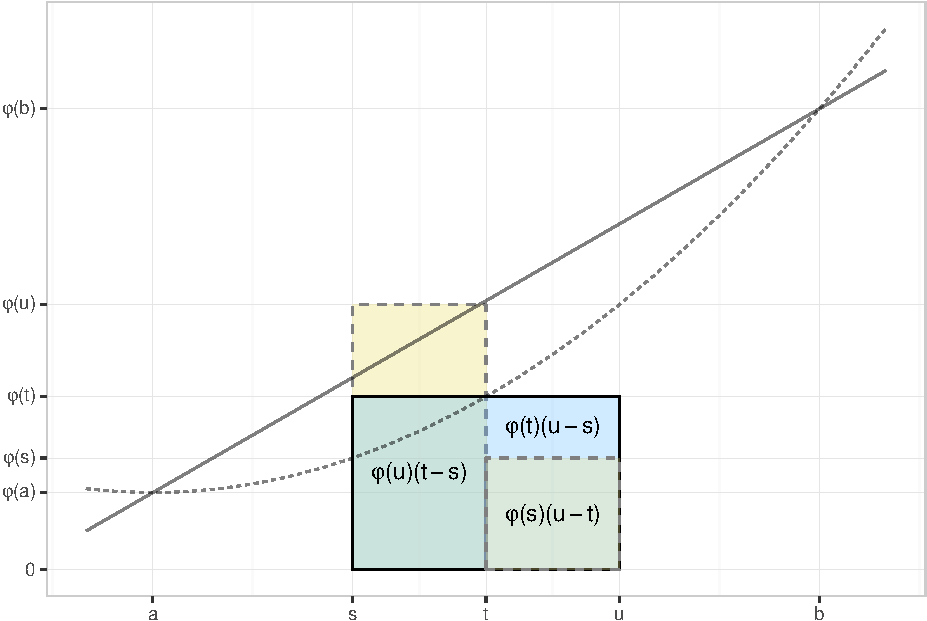
\includegraphics{Glósur_MogT_files/figure-latex/unnamed-chunk-7-1.pdf}

\begin{enumerate}
\def\labelenumi{\arabic{enumi}.}
\setcounter{enumi}{1}
\tightlist
\item
  Fæst með því að að velja \(x,y\in(a,b), x>y\) og skoða ójöfnuna
\end{enumerate}

\[
\begin{aligned}
F(x, x+\varepsilon) \leq F(y, y+\varepsilon), \quad x < x + \varepsilon \leq y < y + \varepsilon.
\end{aligned}
\]

fyrir gefið \(\varepsilon > 0\).

\begin{enumerate}
\def\labelenumi{\arabic{enumi}.}
\setcounter{enumi}{2}
\tightlist
\item
  Allar tölur \(x\in(a,b)\) má skrifa á forminu \(x = \lambda a + (1 - \lambda)b\) þar sem \(\lambda\in(0,1)\). Fáum þá
\end{enumerate}

\[
\begin{aligned}
\frac{\varphi(x) - \varphi(a)}{x - a} &= \frac{\varphi(\lambda a + (1 - \lambda)b) - \varphi(a)}{\lambda a + (1 - \lambda)b - a} \\
&\leq \frac{\lambda \varphi(a) + (1 - \lambda)\varphi(b) - \varphi(a)}{\lambda a + (1 - \lambda)b - a} \\
&= \frac{(\lambda - 1) \varphi(a) + (1 - \lambda)\varphi(b)}{(\lambda - 1)a + (1 - \lambda)b} \\
&= \frac{(1 - \lambda)(\varphi(b) -\varphi(a))}{(1 - \lambda)(b - a)} \\
&= \frac{\varphi(b) - \varphi(a)}{b - a}
\end{aligned}
\]

\hypertarget{dmi-3-6}{%
\section*{Dæmi 3}\label{dmi-3-6}}
\addcontentsline{toc}{section}{Dæmi 3}

Látum \((\Omega,\mathcal F,\mu)\) vera málrúm og \(f\in\mathcal L(\Omega,\mu)\). Sýnið að fyrir sérhvert \(\varepsilon > 0\) sé til \(\delta > 0\), sem fullnægur eftirfarandi skilyrði:

\[
\int_E |f|d\mu < \varepsilon \quad \text{fyrir öll } E\in\mathcal F, \text{ sem uppfylla } \mu(E)>\delta.
\]

\hypertarget{lausn-3}{%
\subsection*{Lausn}\label{lausn-3}}
\addcontentsline{toc}{subsection}{Lausn}

\begin{center}\rule{0.5\linewidth}{\linethickness}\end{center}

\hypertarget{dmi-4-6}{%
\section*{Dæmi 4}\label{dmi-4-6}}
\addcontentsline{toc}{section}{Dæmi 4}

Látum \((\Omega,\mathcal F,\mu)\) vera málrúm. Sýnið að sérhvert \(f\in\mathcal L^1(\Omega,\mu)\) fullnægi skilyrðinu

\[
\lim_{x\rightarrow\infty}x\mu(f^{-1}([x,\infty)) = 0.
\]

Er mælanlegt fall á \(\Omega\) heildanlegt ef það uppfyllir umrætt skilyrði?

\hypertarget{lausn-4}{%
\subsection*{Lausn}\label{lausn-4}}
\addcontentsline{toc}{subsection}{Lausn}

\begin{center}\rule{0.5\linewidth}{\linethickness}\end{center}

\hypertarget{dmi-5-skil}{%
\section*{Dæmi 5 (Skil)}\label{dmi-5-skil}}
\addcontentsline{toc}{section}{Dæmi 5 (Skil)}

Sýnið með dæmi að niðurstaðan í \emph{dæmi 8.11} sé ekki rétt ef skilyrðinu

\[
\int_\Omega fd\mu < \infty
\]

er sleppt.

\hypertarget{lausn-5}{%
\subsection*{Lausn}\label{lausn-5}}
\addcontentsline{toc}{subsection}{Lausn}

\begin{center}\rule{0.5\linewidth}{\linethickness}\end{center}

\hypertarget{dmi-6-6}{%
\section*{Dæmi 6}\label{dmi-6-6}}
\addcontentsline{toc}{section}{Dæmi 6}

Látum \((\Omega,\mathcal F,\mu)\) vera málrúm og \(f\in\mathcal L^1(\Omega,\mu)\). Sannið eftirfarandi fullyrðingar.

\begin{enumerate}
\def\labelenumi{\arabic{enumi}.}
\item
  Fyrir sérhverja rauntölu \(a > 0\) hefur mengið \(\{x\in\Omega| |f(x)|\geq a\}\) endanlegt mál.
\item
  Mengið \(\{x\in\Omega|f(x)\neq 0\}\) er teljanlegt sammengi mengja sem hvert um sig er mælanlegt og hefur endanlegt mál. (Slík mengi eru sögð hafa \(\mathbf \sigma\)\textbf{-endanlegt} mál).
\end{enumerate}

\hypertarget{verstalaar-fjolskyldur}{%
\chapter{Þverstaðlaðar fjölskyldur}\label{verstalaar-fjolskyldur}}

Í þessari grein táknar \(H\) ávalt Hilbert-rúm.

\hypertarget{skilgreining-28}{%
\section*{Skilgreining}\label{skilgreining-28}}
\addcontentsline{toc}{section}{Skilgreining}

Fjölskylda \((u_\alpha)_{\alpha\in A}\) í \(H\) er sögð \textbf{þverstöðluð} ef um öll \(\alpha\) og \(\beta\) úr A gildir

\[
\langle u_\alpha, u_\beta\rangle = 
\begin{cases}
1, \text{ ef } \alpha = \beta \\
0, \text{ ef } \alpha \neq \beta
\end{cases}
\]

Hugtökin \textbf{þverstöðluð upptalning}, \textbf{þverstöðluð runa} og \textbf{þverstaðlað mengi} eru skilgreind á samsvarandi hátt.

\hypertarget{setning-82}{%
\section*{Setning}\label{setning-82}}
\addcontentsline{toc}{section}{Setning}

Látum \(u_1, \dots, u_k\) vera þverstaðlaða upptalningu í \(H\) og \(x = \sum_{j=1}^k c_ju_j\). Þá gildir

\begin{enumerate}
\def\labelenumi{\arabic{enumi}.}
\item
  \(c_j = \langle x,u_j\rangle\) fyrir öll \(j\) úr \(\{1, \dots, k\}\)
\item
  \(\Vert x\Vert^2 = \sum_{j=1}^k\vert c_j\vert^2\).
\end{enumerate}

\begin{center}\rule{0.5\linewidth}{\linethickness}\end{center}

\textbf{Sönnun.}

\begin{center}\rule{0.5\linewidth}{\linethickness}\end{center}

\hypertarget{setning-83}{%
\section*{Setning}\label{setning-83}}
\addcontentsline{toc}{section}{Setning}

Þverstaðlaðar fjölskyldur í Hilbert-rúmum eru línulega óháðar.

\begin{center}\rule{0.5\linewidth}{\linethickness}\end{center}

\textbf{Sönnun.}

\begin{center}\rule{0.5\linewidth}{\linethickness}\end{center}

\hypertarget{setning-84}{%
\section*{Setning}\label{setning-84}}
\addcontentsline{toc}{section}{Setning}

Látum \((V,\Vert\cdot\Vert)\) vera staðlað rúm af endanlegri vídd.

\begin{enumerate}
\def\labelenumi{\arabic{enumi}.}
\tightlist
\item
  Allar línulegar varpanir frá \(V\) inn í staðlað rúm eru samfelldar.
\item
  \(V\) er fullkomið firðrúm.
\end{enumerate}

\begin{center}\rule{0.5\linewidth}{\linethickness}\end{center}

\textbf{Sönnun.}

\begin{center}\rule{0.5\linewidth}{\linethickness}\end{center}

\hypertarget{setning-85}{%
\section*{Setning}\label{setning-85}}
\addcontentsline{toc}{section}{Setning}

Látum \(u_1, \dots, u_k\) vera þverstaðlaða upptalningu í \(H\). Látum \(K\) vera (lokaða) hlutrúmið sem hún spannar og \(P:H\rightarrow H\) tákna hornrétta ofanvarpið á \(K\). Þá gildir um öll \(x\) úr \(H\):

\[
P(x) = \sum_{j=1}^k\langle x,u_j\rangle u_j.
\]

\begin{center}\rule{0.5\linewidth}{\linethickness}\end{center}

\textbf{Sönnun.}

\begin{center}\rule{0.5\linewidth}{\linethickness}\end{center}

\hypertarget{setning-86}{%
\section*{Setning}\label{setning-86}}
\addcontentsline{toc}{section}{Setning}

Látum \((u_\alpha)_{\alpha\in A}\) vera þverstaðlaða fjölskyldu í \(H\). Þá gildir um sérhvert endanlegt hlutmengi \(I\) í \(A\) og öll \(X\) úr \(H\):

\[
\sum_{\alpha\in I}\vert\langle x,u_\alpha\rangle\vert^2\leq\Vert x\Vert^2
\]

Ójafnan er yfirleitt kölluð \textbf{Bessel-ójafna}.

\begin{center}\rule{0.5\linewidth}{\linethickness}\end{center}

\hypertarget{vikubla-11}{%
\chapter*{Vikublað 11}\label{vikubla-11}}
\addcontentsline{toc}{chapter}{Vikublað 11}

\hypertarget{dmi-1-skil-1}{%
\section*{Dæmi 1 (Skil)}\label{dmi-1-skil-1}}
\addcontentsline{toc}{section}{Dæmi 1 (Skil)}

Látum \((\Omega,\mathcal F, \mu)\) vera líkindarúm og \(h:\Omega\rightarrow[0,\infty)\) vera heildanlegt fall. Setjum \(A:=\int_\Omega hd\mu\).

\begin{enumerate}
\def\labelenumi{\arabic{enumi}.}
\item
  Sýnið að \(\sqrt{1 + A^2} \leq \int_\Omega\sqrt{1 + h^2}d\mu\leq 1 + A\)
\item
  Skoðum nú sértilfellið þegar \(\Omega\) er lokaða bilið \([0,1]\) með venjulega Lebesgue-málinu og gerum ennfremur ráð fyrir að \(h = f'\) þar sem \(f\) er samfellt diffranlegt fall á \([0,1]\). Túlkið ójöfnurnar í lið \emph{1.} út frá fallriti fallsins \(f\) og segið síðan til um hvenær jafnaðarmerki gildir í hvorri ójöfnu fyrir sig.
\end{enumerate}

\begin{center}\rule{0.5\linewidth}{\linethickness}\end{center}

\textbf{Lausn.}

\begin{center}\rule{0.5\linewidth}{\linethickness}\end{center}

\hypertarget{dmi-2-skil-1}{%
\section*{Dæmi 2 (Skil)}\label{dmi-2-skil-1}}
\addcontentsline{toc}{section}{Dæmi 2 (Skil)}

Sýnið að fallið

\[
f:(0,\infty)\rightarrow\mathbb R, \quad x\rightarrow\frac{1}{\sqrt x + \vert\log x\vert}
\]

sé í \(L^p((0,\infty))\) þá og því aðeins að \(p>2\).

\begin{center}\rule{0.5\linewidth}{\linethickness}\end{center}

\textbf{Sönnun.}

\begin{center}\rule{0.5\linewidth}{\linethickness}\end{center}

\hypertarget{dmi-5-skil-1}{%
\section*{Dæmi 5 (Skil)}\label{dmi-5-skil-1}}
\addcontentsline{toc}{section}{Dæmi 5 (Skil)}

Látum \((f_n)_{n\geq1}\) vera runu af tvinngildum mælanlegum föllum á \emph{takmörkuðu málrúmi} \((\Omega,\mathcal F,\mu)\) (þ.e.a.s. \(\mu(\Omega)<\infty\)) og gerum ráð fyrir að hún stefni (í sérhverjum punkti) á fall \(f\).

\begin{enumerate}
\def\labelenumi{\arabic{enumi}.}
\tightlist
\item
  Sýnið að fyrir sérhvert \(\varepsilon > 0\) sé til \(E\) úr \(\mathcal F\) sem uppfyllir eftirtalin skilyrði:
\end{enumerate}

\begin{itemize}
\tightlist
\item
  \(\mu(\Omega\backslash E) < \varepsilon\)
\item
  \(f_n \rightarrow f\) í jöfnum mæli á \(E\).
\end{itemize}

\emph{Ábending:} Setjið \(S(n,k) := \bigcap_{j<n}\left\{x\in \Omega: \vert f(x) - f_j(x)\vert < \frac1k \right\}\) og sýnið að fyrir sérhvert \(k\) gildi \(\lim_{n\rightarrow}\mu(S(n,k)) = \mu(\Omega)\)

\begin{enumerate}
\def\labelenumi{\arabic{enumi}.}
\setcounter{enumi}{1}
\tightlist
\item
  Sýnið með dæmi að niðurstaðan sé almennt ekki rétt fyrir ótakmörkuð málrúm.
\end{enumerate}

\hypertarget{dmi-8-skil}{%
\section*{Dæmi 8 (Skil)}\label{dmi-8-skil}}
\addcontentsline{toc}{section}{Dæmi 8 (Skil)}

Látum \(\lambda\) vera málið á \((\mathbb N^*, \mathcal P(\mathbb N^*))\) sem ákvarðast af \(\lambda(\{n\}) = \frac{1}{n^2}\) og setjum

\[
 f:\mathbb N^*\rightarrow\mathbb R, \quad n\rightarrow\sqrt n.
\]

Sýnið að \(f\in\mathcal L^p(\mathbb N^*,\lambda)\) þá og því aðeins að \(1\leq p< 2\).

\begin{center}\rule{0.5\linewidth}{\linethickness}\end{center}

\textbf{Lausn.}

\begin{center}\rule{0.5\linewidth}{\linethickness}\end{center}


\end{document}
